% Options for packages loaded elsewhere
\PassOptionsToPackage{unicode}{hyperref}
\PassOptionsToPackage{hyphens}{url}
%
\documentclass[
]{book}
\usepackage{lmodern}
\usepackage{amsmath}
\usepackage{ifxetex,ifluatex}
\ifnum 0\ifxetex 1\fi\ifluatex 1\fi=0 % if pdftex
  \usepackage[T1]{fontenc}
  \usepackage[utf8]{inputenc}
  \usepackage{textcomp} % provide euro and other symbols
  \usepackage{amssymb}
\else % if luatex or xetex
  \usepackage{unicode-math}
  \defaultfontfeatures{Scale=MatchLowercase}
  \defaultfontfeatures[\rmfamily]{Ligatures=TeX,Scale=1}
\fi
% Use upquote if available, for straight quotes in verbatim environments
\IfFileExists{upquote.sty}{\usepackage{upquote}}{}
\IfFileExists{microtype.sty}{% use microtype if available
  \usepackage[]{microtype}
  \UseMicrotypeSet[protrusion]{basicmath} % disable protrusion for tt fonts
}{}
\makeatletter
\@ifundefined{KOMAClassName}{% if non-KOMA class
  \IfFileExists{parskip.sty}{%
    \usepackage{parskip}
  }{% else
    \setlength{\parindent}{0pt}
    \setlength{\parskip}{6pt plus 2pt minus 1pt}}
}{% if KOMA class
  \KOMAoptions{parskip=half}}
\makeatother
\usepackage{xcolor}
\IfFileExists{xurl.sty}{\usepackage{xurl}}{} % add URL line breaks if available
\IfFileExists{bookmark.sty}{\usepackage{bookmark}}{\usepackage{hyperref}}
\hypersetup{
  pdftitle={industRial data science},
  pdfauthor={João Ramalho},
  hidelinks,
  pdfcreator={LaTeX via pandoc}}
\urlstyle{same} % disable monospaced font for URLs
\usepackage{color}
\usepackage{fancyvrb}
\newcommand{\VerbBar}{|}
\newcommand{\VERB}{\Verb[commandchars=\\\{\}]}
\DefineVerbatimEnvironment{Highlighting}{Verbatim}{commandchars=\\\{\}}
% Add ',fontsize=\small' for more characters per line
\usepackage{framed}
\definecolor{shadecolor}{RGB}{248,248,248}
\newenvironment{Shaded}{\begin{snugshade}}{\end{snugshade}}
\newcommand{\AlertTok}[1]{\textcolor[rgb]{0.94,0.16,0.16}{#1}}
\newcommand{\AnnotationTok}[1]{\textcolor[rgb]{0.56,0.35,0.01}{\textbf{\textit{#1}}}}
\newcommand{\AttributeTok}[1]{\textcolor[rgb]{0.77,0.63,0.00}{#1}}
\newcommand{\BaseNTok}[1]{\textcolor[rgb]{0.00,0.00,0.81}{#1}}
\newcommand{\BuiltInTok}[1]{#1}
\newcommand{\CharTok}[1]{\textcolor[rgb]{0.31,0.60,0.02}{#1}}
\newcommand{\CommentTok}[1]{\textcolor[rgb]{0.56,0.35,0.01}{\textit{#1}}}
\newcommand{\CommentVarTok}[1]{\textcolor[rgb]{0.56,0.35,0.01}{\textbf{\textit{#1}}}}
\newcommand{\ConstantTok}[1]{\textcolor[rgb]{0.00,0.00,0.00}{#1}}
\newcommand{\ControlFlowTok}[1]{\textcolor[rgb]{0.13,0.29,0.53}{\textbf{#1}}}
\newcommand{\DataTypeTok}[1]{\textcolor[rgb]{0.13,0.29,0.53}{#1}}
\newcommand{\DecValTok}[1]{\textcolor[rgb]{0.00,0.00,0.81}{#1}}
\newcommand{\DocumentationTok}[1]{\textcolor[rgb]{0.56,0.35,0.01}{\textbf{\textit{#1}}}}
\newcommand{\ErrorTok}[1]{\textcolor[rgb]{0.64,0.00,0.00}{\textbf{#1}}}
\newcommand{\ExtensionTok}[1]{#1}
\newcommand{\FloatTok}[1]{\textcolor[rgb]{0.00,0.00,0.81}{#1}}
\newcommand{\FunctionTok}[1]{\textcolor[rgb]{0.00,0.00,0.00}{#1}}
\newcommand{\ImportTok}[1]{#1}
\newcommand{\InformationTok}[1]{\textcolor[rgb]{0.56,0.35,0.01}{\textbf{\textit{#1}}}}
\newcommand{\KeywordTok}[1]{\textcolor[rgb]{0.13,0.29,0.53}{\textbf{#1}}}
\newcommand{\NormalTok}[1]{#1}
\newcommand{\OperatorTok}[1]{\textcolor[rgb]{0.81,0.36,0.00}{\textbf{#1}}}
\newcommand{\OtherTok}[1]{\textcolor[rgb]{0.56,0.35,0.01}{#1}}
\newcommand{\PreprocessorTok}[1]{\textcolor[rgb]{0.56,0.35,0.01}{\textit{#1}}}
\newcommand{\RegionMarkerTok}[1]{#1}
\newcommand{\SpecialCharTok}[1]{\textcolor[rgb]{0.00,0.00,0.00}{#1}}
\newcommand{\SpecialStringTok}[1]{\textcolor[rgb]{0.31,0.60,0.02}{#1}}
\newcommand{\StringTok}[1]{\textcolor[rgb]{0.31,0.60,0.02}{#1}}
\newcommand{\VariableTok}[1]{\textcolor[rgb]{0.00,0.00,0.00}{#1}}
\newcommand{\VerbatimStringTok}[1]{\textcolor[rgb]{0.31,0.60,0.02}{#1}}
\newcommand{\WarningTok}[1]{\textcolor[rgb]{0.56,0.35,0.01}{\textbf{\textit{#1}}}}
\usepackage{longtable,booktabs}
\usepackage{calc} % for calculating minipage widths
% Correct order of tables after \paragraph or \subparagraph
\usepackage{etoolbox}
\makeatletter
\patchcmd\longtable{\par}{\if@noskipsec\mbox{}\fi\par}{}{}
\makeatother
% Allow footnotes in longtable head/foot
\IfFileExists{footnotehyper.sty}{\usepackage{footnotehyper}}{\usepackage{footnote}}
\makesavenoteenv{longtable}
\usepackage{graphicx}
\makeatletter
\def\maxwidth{\ifdim\Gin@nat@width>\linewidth\linewidth\else\Gin@nat@width\fi}
\def\maxheight{\ifdim\Gin@nat@height>\textheight\textheight\else\Gin@nat@height\fi}
\makeatother
% Scale images if necessary, so that they will not overflow the page
% margins by default, and it is still possible to overwrite the defaults
% using explicit options in \includegraphics[width, height, ...]{}
\setkeys{Gin}{width=\maxwidth,height=\maxheight,keepaspectratio}
% Set default figure placement to htbp
\makeatletter
\def\fps@figure{htbp}
\makeatother
\setlength{\emergencystretch}{3em} % prevent overfull lines
\providecommand{\tightlist}{%
  \setlength{\itemsep}{0pt}\setlength{\parskip}{0pt}}
\setcounter{secnumdepth}{5}
\ifluatex
  \usepackage{selnolig}  % disable illegal ligatures
\fi
\newlength{\cslhangindent}
\setlength{\cslhangindent}{1.5em}
\newlength{\csllabelwidth}
\setlength{\csllabelwidth}{3em}
\newenvironment{CSLReferences}[2] % #1 hanging-ident, #2 entry spacing
 {% don't indent paragraphs
  \setlength{\parindent}{0pt}
  % turn on hanging indent if param 1 is 1
  \ifodd #1 \everypar{\setlength{\hangindent}{\cslhangindent}}\ignorespaces\fi
  % set entry spacing
  \ifnum #2 > 0
  \setlength{\parskip}{#2\baselineskip}
  \fi
 }%
 {}
\usepackage{calc}
\newcommand{\CSLBlock}[1]{#1\hfill\break}
\newcommand{\CSLLeftMargin}[1]{\parbox[t]{\csllabelwidth}{#1}}
\newcommand{\CSLRightInline}[1]{\parbox[t]{\linewidth - \csllabelwidth}{#1}\break}
\newcommand{\CSLIndent}[1]{\hspace{\cslhangindent}#1}

\title{industRial data science}
\usepackage{etoolbox}
\makeatletter
\providecommand{\subtitle}[1]{% add subtitle to \maketitle
  \apptocmd{\@title}{\par {\large #1 \par}}{}{}
}
\makeatother
\subtitle{Case studies in product development and manufacturing}
\author{João Ramalho}
\date{2021-03-15}

\begin{document}
\maketitle

{
\setcounter{tocdepth}{1}
\tableofcontents
}
\hypertarget{introduction}{%
\chapter*{Introduction}\label{introduction}}
\addcontentsline{toc}{chapter}{Introduction}

\hypertarget{objectives}{%
\section{Objectives}\label{objectives}}

This book provides examples on how to use Data Science tools and techniques in Product Development and Manufacturing. The case studies are presented in a ``cookbook'' approach, making it easier to directly adopt the tools. They come from varied manufacturing industries, mostly where repetitive production in massive quantities is involved, such as:

\begin{itemize}
\tightlist
\item
  pharmaceuticals
\item
  food
\item
  electronics
\item
  watch making
\item
  automotive
\end{itemize}

Product Development and Manufacturing are very important activities in society because bringing innovative products to the market has an immense potential to improve the quality of life of everyone.

Additionally Data Science brings new powerful approaches to the engineering and manufacturing of consumer goods, helping minimising environmental impact, improving quality and keeping costs under control.

\hypertarget{background-knowledge}{%
\section{Background knowledge}\label{background-knowledge}}

In this book it is assumed that the reader is already familiar with the product development and manufacturing quality methodologies such as dmaic and six sigma and the associated statistical concepts. Furthermore it is considered that he brings at least a beginner knowledge on R. The book focus is then on putting the different areas together.

\hypertarget{six-sigma}{%
\subsection{Six Sigma}\label{six-sigma}}

Below a selection of Six Sigma tools relevant for our case studies and describing how they can help framing the data analysis presented throughout the rest of book. These tools support the Design for Six Sigma methodology that links the features of a product with its production process. One way of summarising the Six Sigma framework is the following:

Voice of Customer

\begin{enumerate}
\def\labelenumi{\arabic{enumi}.}
\tightlist
\item
  Product attributes
\item
  Functional analysis
\item
  Functional requirements
\item
  Failure modes and effects analysis (FMEA)
\item
  Product parts drawings
\end{enumerate}

Voice of Process

\begin{enumerate}
\def\labelenumi{\arabic{enumi}.}
\tightlist
\item
  Equipement drawings
\item
  Process mapping
\item
  Process FMEA
\item
  Control plan
\item
  Measurement system analysis
\item
  Process capability
\end{enumerate}

Each of this steps comprises important analyis of the product and process characteristics. For a more detailed description we recommend reviewing the comprehensive Six Sigma certification reference book by \protect\hyperlink{ref-Munro2015}{Roderik A.Munro and J.Zrymiak} (\protect\hyperlink{ref-Munro2015}{2015}).

\hypertarget{statistics}{%
\subsection{Statistics}\label{statistics}}

The key statistical concepts used throughout this book are listed below:

\textbf{Descriptive statistics}

\begin{itemize}
\tightlist
\item
  mean
\item
  median
\item
  mode
\item
  variance
\item
  standard deviation
\item
  range
\end{itemize}

\textbf{Modeling data distributions}

\begin{itemize}
\tightlist
\item
  Normal distribution
\item
  Central limit theorem
\item
  Confidence intervals
\item
  Linear Models
\end{itemize}

\textbf{Significance tests}

\begin{itemize}
\tightlist
\item
  comparing means
\item
  comparing variances
\item
  linear models
\item
  Anova
\item
  Ancova
\end{itemize}

For a deep and comprehensive course on statistics we recommend the free online \href{https://www.khanacademy.org/math/statistics-probability}{kahn academy} courses.

\hypertarget{r-programming}{%
\subsection{R programming}\label{r-programming}}

Why R? Many tools exist to do Data Analysis and Statistics with different degrees of power and difficulty such as:

\begin{itemize}
\tightlist
\item
  Spreadsheets: Excel, Libreoffice, Numbers
\item
  Proprietary software: Minitab, Mathlab
\item
  Programming languages: Visual Basic, R, Python, Julia
\item
  Databases: sqlite, postgre, mysql, mongodb
\end{itemize}

Choosing the right set of tools for Data Science is often not a very scientific task. Mostly is a matter of what is available and what our colleagues, customers or suppliers use. As with everything it is important to remain open to evaluate new tools and approaches and even to be able to combine them.

In this book we've chosen to provide all examples in R which is a free software environment for statistical computing and graphics \url{https://www.r-project.org/}
Besides taste and personnal preference R brings a significant number of specific advantages in the field of Industrial Data Science:

\begin{enumerate}
\def\labelenumi{\arabic{enumi}.}
\tightlist
\item
  R allows for reproducible research
\end{enumerate}

This because the algorithms and functions defined to make the calculations can be inspected and all results can be fully reproduced and audited. This is known as reproducible research and is a critical aspect in all areas where a proof is needed such as in equipment validation and product quality reporting.

\begin{enumerate}
\def\labelenumi{\arabic{enumi}.}
\setcounter{enumi}{1}
\tightlist
\item
  R functions, tools and programs can be adapted and improved
\end{enumerate}

Being an open source language, all R libraries and packages added to the basic environment can be not only audited but adapted and improved This is very important as when we enter into details every industry has a slight different way of doing things, different naming conventions, different coeficients and so on.

\begin{enumerate}
\def\labelenumi{\arabic{enumi}.}
\setcounter{enumi}{2}
\tightlist
\item
  R is extensible
\end{enumerate}

R is compatible with most other software on the market and is an excellent ``glue'' tool allowing for example for data loading from excel files, producing reports in pdf and even building complete dashboards in the form of web pages.

When selecting new packages it is recommended to check the latest package update. Packages that have had no improvements since more than a couple of years should be questionned. The field evolves rapidly and compatibility and other issues can become painfull. A way to obtain statistics on package history is on \href{https://www.r-pkg.org/}{metacran}. A comprehensive list of the different packages used in the book and how to obtain them is available in the toolbox chapter.

This book has been entirely written with the excellent R package Bookdown from Yihui Xie (\protect\hyperlink{ref-Xie2016}{Xie 2016}), that has the ability of automatically generate reports with plots and text together.

\hypertarget{how-to-use-this-book}{%
\section{How to use this book}\label{how-to-use-this-book}}

Being a collection of case studies, the book is better used as a reference book. There are the following ways to get to the desired topic:

\begin{itemize}
\tightlist
\item
  Table of contents
\item
  R function index
\item
  R package index
\end{itemize}

Additionally we refer to several good quality books on both Data Science and Product Development that have served to provide the required theoretical background. These cover key disciplines such as six sigma, statistics and computer programming. Our book aims complementing them and showcase how to benefit from recent software in this area.

\hypertarget{about-the-authors}{%
\section{About the authors}\label{about-the-authors}}

João Ramalho is a Senior Industrial Data Scientist with more than 20 years of experience in the manufacturing industry. He's been in varied positions in R\&D, Operations and IT at Philip Morris, Rolex and Nestlé. He holds a Master in Mechanical Engineering from the IST of Lisbon, a PMP certification from the Project Management Institute and a Data Science certification from DataCamp. He's currently specializing in Data Visualization at the Swiss technical university EPFL. See full profile at \href{https://j-ramalho.github.io/}{j-ramalho.github.io}

\hypertarget{part-case-studies}{%
\part{CASE STUDIES}\label{part-case-studies}}

\hypertarget{s---six-sigma}{%
\chapter{6S - Six Sigma}\label{s---six-sigma}}

\hypertarget{pareto}{%
\section{Pareto}\label{pareto}}

The pareto chart has always proven an effective way of defining priorities and keeping workload under control. It is known for helping focusing on the few important elements that account for most problems. It builds on the well known insight that a few reasons explain or allow to control most of the outcome. This applies particularly well in the technological and industrial context.

The example here comes from a dial polishing workshop in the watchmaking industry. Dials are received from the stamping process and polished before being sent to the final assembly. As part of the authonomous quality control performed by the polishing operators a count of the defects observed on the dials each day is kept in a file.

\begin{figure}

{\centering 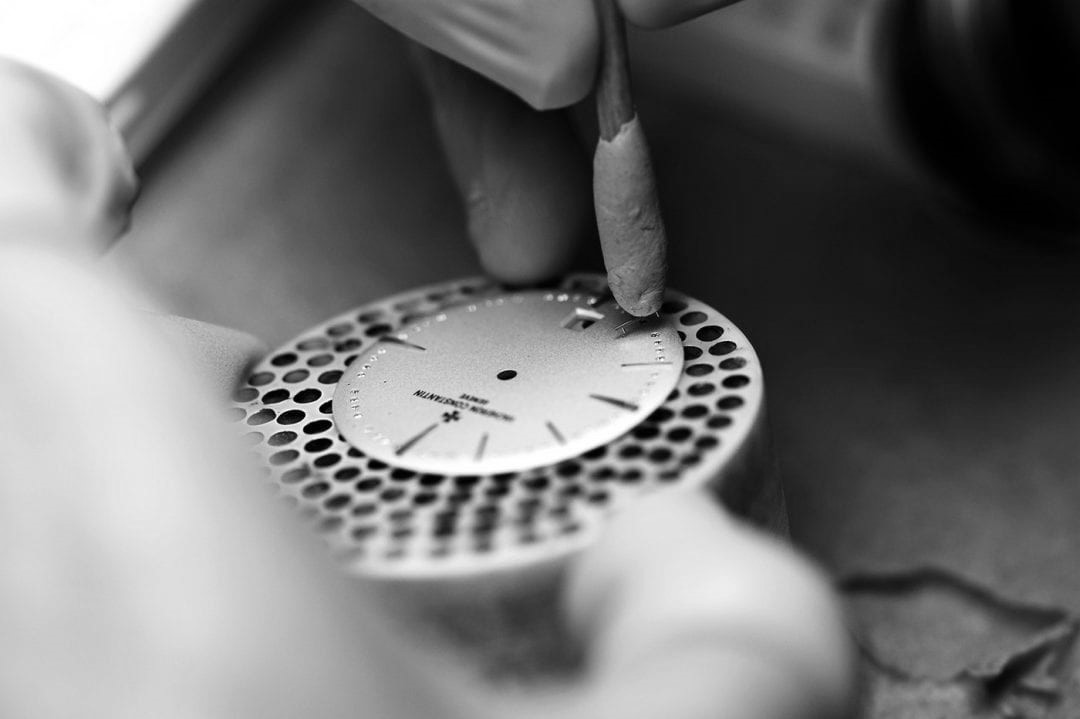
\includegraphics[width=0.6\linewidth]{img/assemblage_cadran_bw} 

}

\caption{watch dial inspection}\label{fig:unnamed-chunk-2}
\end{figure}

Loading packages and data:

Loading the data:

Getting the book companion package from github:

\begin{verbatim}
devtools::install_github("J-Ramalho/industRial")
\end{verbatim}

load it in the current session:

\begin{Shaded}
\begin{Highlighting}[]
\FunctionTok{library}\NormalTok{(industRial)}
\end{Highlighting}
\end{Shaded}

getting the dial dataset:

\begin{Shaded}
\begin{Highlighting}[]
\NormalTok{dial\_control }\OtherTok{\textless{}{-}}\NormalTok{  industRial}\SpecialCharTok{::}\NormalTok{dial\_control}
\end{Highlighting}
\end{Shaded}

\begin{Shaded}
\begin{Highlighting}[]
\FunctionTok{library}\NormalTok{(tidyverse)}
\FunctionTok{library}\NormalTok{(qicharts2)}
\FunctionTok{library}\NormalTok{(knitr)}
\end{Highlighting}
\end{Shaded}

\begin{Shaded}
\begin{Highlighting}[]
\FunctionTok{head}\NormalTok{(dial\_control) }\SpecialCharTok{\%\textgreater{}\%} 
  \FunctionTok{kable}\NormalTok{(}\AttributeTok{align =} \StringTok{"c"}\NormalTok{, }
        \AttributeTok{caption =} \StringTok{"dial control data"}\NormalTok{, }
        \AttributeTok{booktabs =}\NormalTok{ T)}
\end{Highlighting}
\end{Shaded}

\begin{table}

\caption{\label{tab:tab-dial}dial control data}
\centering
\begin{tabular}[t]{cccc}
\toprule
Operator & Date & Defect & Location\\
\midrule
Jane & 2018.01.31 & Indent & 3\\
Jane & 2018.02.02 & Indent & 3\\
Jane & 2018.02.02 & Indent & 4\\
Peter & 2018.02.02 & Indent & 10\\
Jane & 2018.02.03 & Scratch & 3\\
\addlinespace
Jane & 2018.02.03 & Indent & 3\\
\bottomrule
\end{tabular}
\end{table}

We can see that the count includes both the deffect type and the location (the hour in the dial) and that it is traced to the day and operator.

The team leader promotes a culture of fact based assessment of the quality measurements. Every week the team looks back and observes the weekly counts. This is important because it helps moving away from perception into a more solid assessment. The volume of data is higher like this enabling trends to start becoming apparent. The team can discuss potential actions and prepare reporting to the supplier of the parts (the stamping workshop). It also helps calibrating between operators and agreeing on acceptance criteria and what is and what is not a defect.

A first example of the pareto of the types of defects:

\begin{Shaded}
\begin{Highlighting}[]
\NormalTok{d\_type }\OtherTok{\textless{}{-}}\NormalTok{ dial\_control }\SpecialCharTok{\%\textgreater{}\%} \FunctionTok{pull}\NormalTok{(Defect) }\SpecialCharTok{\%\textgreater{}\%} \FunctionTok{as.character}\NormalTok{()}
\NormalTok{d\_type\_p }\OtherTok{\textless{}{-}} \FunctionTok{paretochart}\NormalTok{(d\_type, }
                           \AttributeTok{title =} \StringTok{"Watch Dial polishing"}\NormalTok{,}
                           \AttributeTok{subtitle =} \StringTok{"Pareto chart"}\NormalTok{, }
                           \AttributeTok{ylab =} \StringTok{"Percentage of deffects"}\NormalTok{,}
                           \AttributeTok{xlab =} \StringTok{"Deffect type"}\NormalTok{,}
                           \AttributeTok{caption =} \StringTok{"Source: Dial Production Team"}\NormalTok{)}
\NormalTok{d\_type\_p}
\end{Highlighting}
\end{Shaded}

\includegraphics[width=0.8\linewidth]{sixsigma_files/figure-latex/unnamed-chunk-6-1}

As often happens we can see that the first two deffects account for more than 80\% of the problems. Identation and scratching are the things to tackle here.

From the available data presented before in table \ref{tab:tab-dial} we can go deeper and establish a pareto of the defect location:

\begin{Shaded}
\begin{Highlighting}[]
\NormalTok{d\_location }\OtherTok{\textless{}{-}}\NormalTok{ dial\_control }\SpecialCharTok{\%\textgreater{}\%} \FunctionTok{pull}\NormalTok{(Location) }\SpecialCharTok{\%\textgreater{}\%} \FunctionTok{as.character}\NormalTok{()}
\NormalTok{d\_location\_p }\OtherTok{\textless{}{-}} \FunctionTok{paretochart}\NormalTok{(d\_location, }
                           \AttributeTok{title =} \StringTok{"Watch Dial polishing"}\NormalTok{,}
                           \AttributeTok{subtitle =} \StringTok{"Pareto chart"}\NormalTok{, }
                           \AttributeTok{ylab =} \StringTok{"Percentage of deffects"}\NormalTok{,}
                           \AttributeTok{xlab =} \StringTok{"Deffect location (hour)"}\NormalTok{,}
                           \AttributeTok{caption =} \StringTok{"Source: Dial Production Team"}\NormalTok{)}
\NormalTok{d\_location\_p}
\end{Highlighting}
\end{Shaded}

\includegraphics[width=0.8\linewidth]{sixsigma_files/figure-latex/unnamed-chunk-7-1}

Here a third bucket could be included in the priorities: to reach 80\% of the count we consider the defects that appear at 4 o'clock, 3 o'clock and 5 o'clock.

During the reviews the team can also identify other types of data for follow up such as the dial model or the material type. With a simple excel file and an upload in R this can be finetuned from week to week according to the progress of the improvement measures.

\hypertarget{ishikawa}{%
\section{Ishikawa}\label{ishikawa}}

Usually called Fishbone or Ishikawa diagrams this simple tool has proven to be extremely practical and helpful in structuring team discussions.

\begin{figure}

{\centering 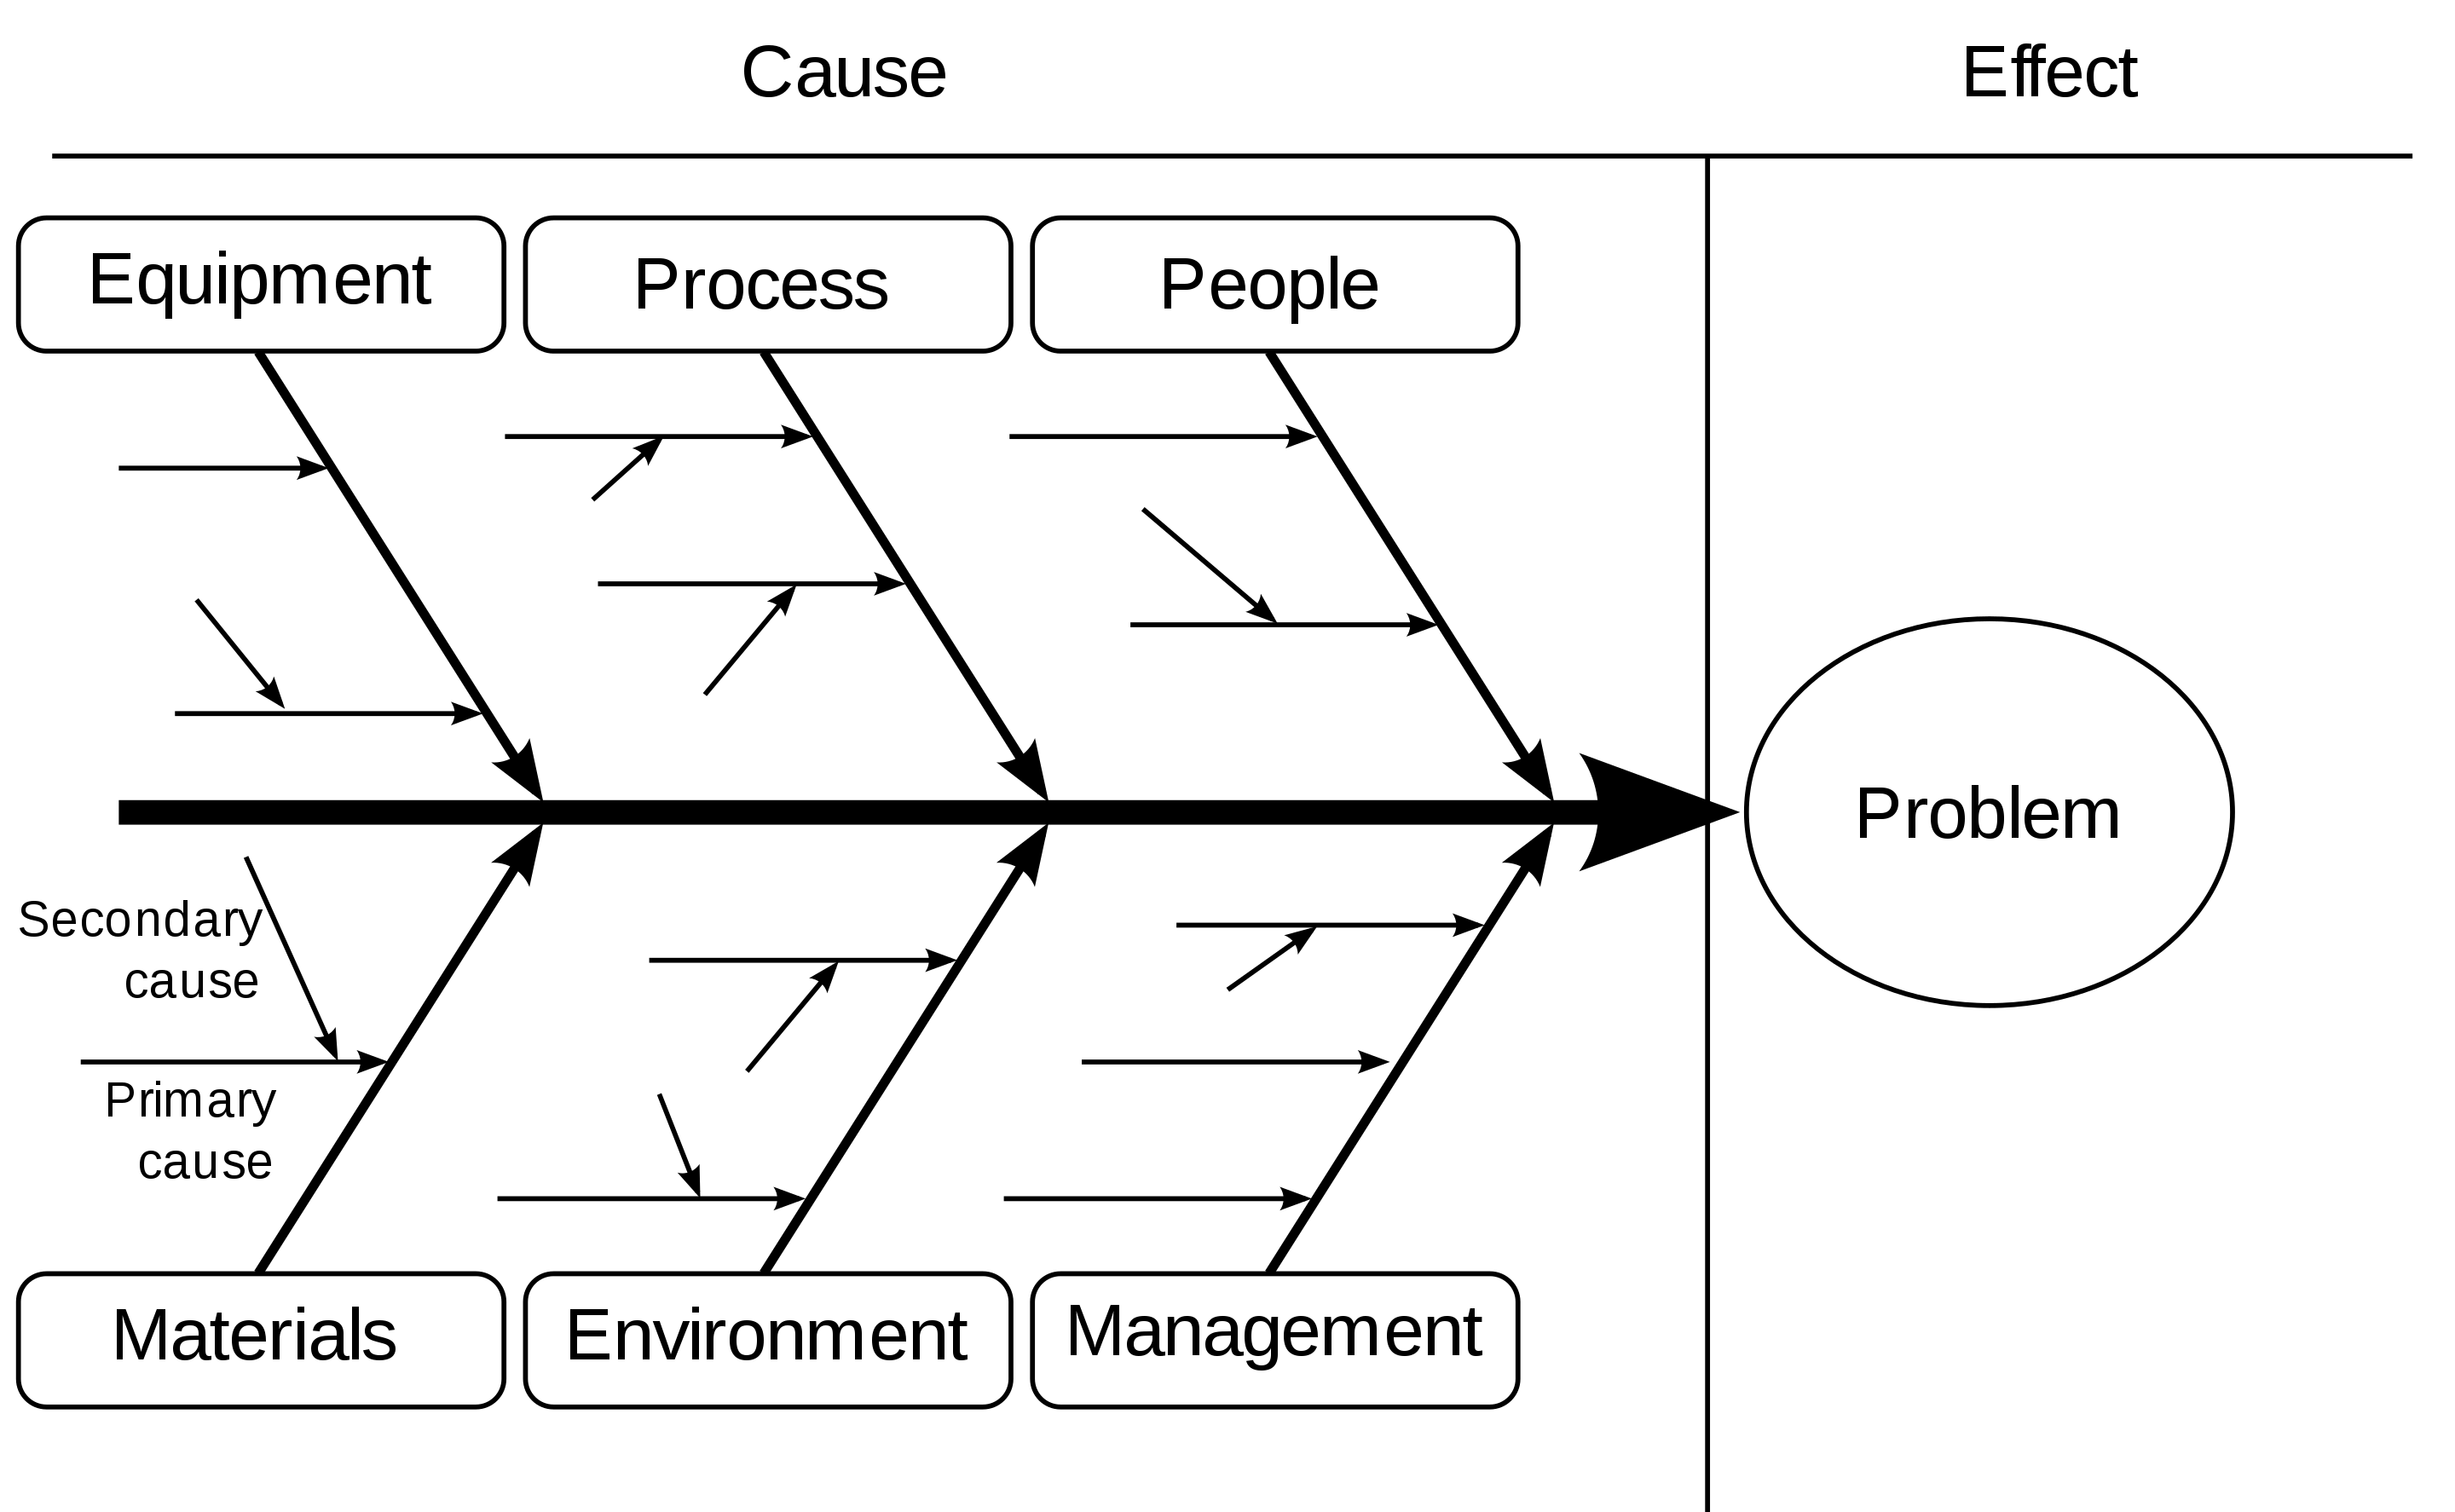
\includegraphics[width=0.6\linewidth]{img/ishikawa} 

}

\caption{ishikawa diagram, source: wikipedia}\label{fig:fig-ishikawa}
\end{figure}

With it we can easily identify and list the expected influencing factors for example to design an experiment. Such selection and grouping of parameters can be useful for among others in defining the right mix of ingredients in a new product or material, in selecting the machine parameters in a manufacturing line or in the definition of a draft operating procedure for a measurement. In each of these situations it helps seeing the big picture and not fall into the trap of relying only in the data and findings obtained by statistical analysis.

\hypertarget{DOE}{%
\chapter{DOE - Design of Experiments}\label{DOE}}

\hypertarget{one-factor-two-levels}{%
\section{One factor two levels}\label{one-factor-two-levels}}

\hypertarget{two-means-comparison}{%
\subsection{Two means comparison}\label{two-means-comparison}}

\hypertarget{tTest}{%
\subsubsection{t-test one sample}\label{tTest}}

Comparing mean to specification

An engineer working the winter sports clothing industry has established a contract for PET textile raw material supply based on the following specification: the average tensile strength has to be greater than 69.0 \(Mpa\) for each delivery. In the contract is also specified that the test protocol which is based on a 30 samples.

\begin{figure}

{\centering 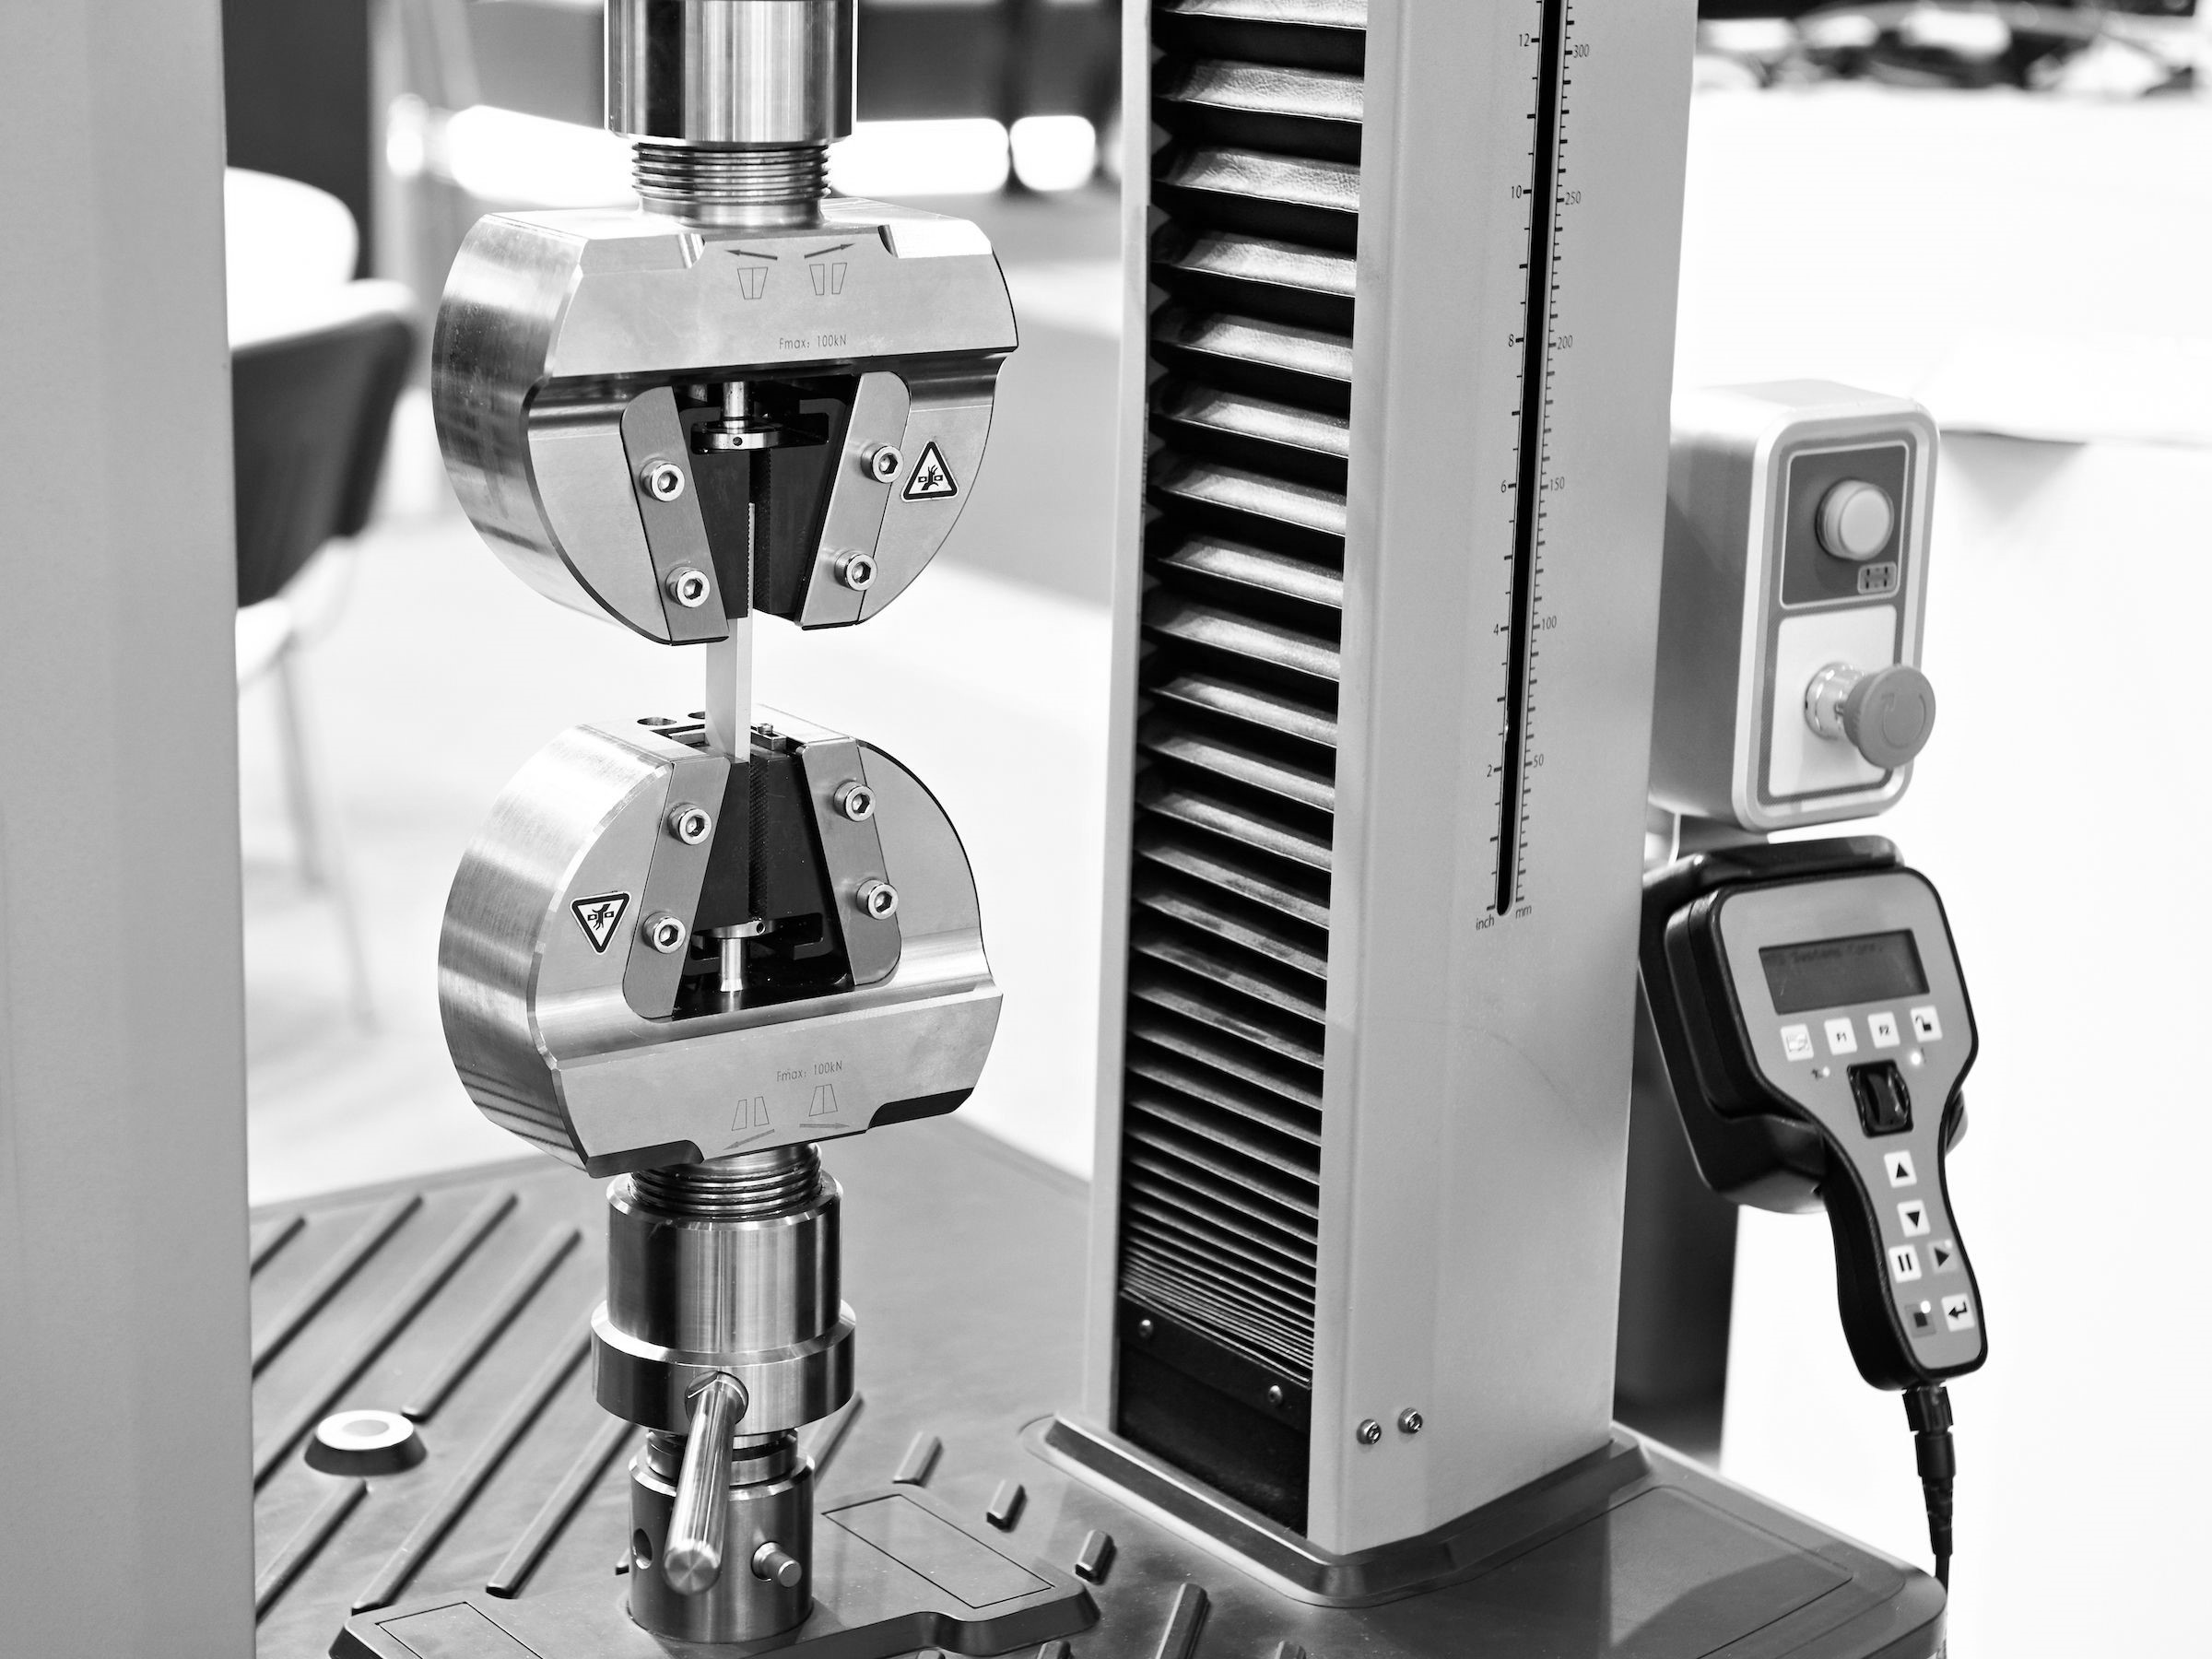
\includegraphics[width=0.6\linewidth]{img/tensile_test_bw} 

}

\caption{PET tensile test}\label{fig:unnamed-chunk-2}
\end{figure}

A first delivery is submited and the customer wants to know if the lot average tensile strength exceeds the agreed level and if so, she wants to accept the lot.

We start by loading the first packages we will need:

\begin{Shaded}
\begin{Highlighting}[]
\FunctionTok{library}\NormalTok{(tidyverse)}
\FunctionTok{library}\NormalTok{(readxl)}
\FunctionTok{library}\NormalTok{(stats)}

\NormalTok{filter }\OtherTok{\textless{}{-}}\NormalTok{ dplyr}\SpecialCharTok{::}\NormalTok{filter}
\NormalTok{select }\OtherTok{\textless{}{-}}\NormalTok{ dplyr}\SpecialCharTok{::}\NormalTok{select}
\end{Highlighting}
\end{Shaded}

\begin{Shaded}
\begin{Highlighting}[]
\FunctionTok{library}\NormalTok{(industRial)}
\NormalTok{pet\_delivery }\OtherTok{\textless{}{-}}\NormalTok{ industRial}\SpecialCharTok{::}\NormalTok{pet\_delivery}
\end{Highlighting}
\end{Shaded}

The Quality Control department specialist at the reception starts by calcultating the average, a first criteria to reject the batch:

\begin{Shaded}
\begin{Highlighting}[]
\FunctionTok{mean}\NormalTok{(pet\_delivery}\SpecialCharTok{$}\NormalTok{strength)}
\end{Highlighting}
\end{Shaded}

\begin{verbatim}
[1] 68.46429
\end{verbatim}

The average is itself below the spec and the engineer could reject the batch right away. She decides nevertheless to observe the variability and for this she decides to plot the raw data on an histogram. An histogram is a very common plot showing counts for selected intervals.

\begin{Shaded}
\begin{Highlighting}[]
\NormalTok{pet\_delivery }\SpecialCharTok{\%\textgreater{}\%} 
  \FunctionTok{ggplot}\NormalTok{(}\FunctionTok{aes}\NormalTok{(}\AttributeTok{x =}\NormalTok{ strength)) }\SpecialCharTok{+}
  \FunctionTok{geom\_histogram}\NormalTok{(}\AttributeTok{fill =} \StringTok{"cadetblue"}\NormalTok{, }
                 \AttributeTok{color =} \StringTok{"grey20"}\NormalTok{) }\SpecialCharTok{+}
  \FunctionTok{theme\_light}\NormalTok{() }\SpecialCharTok{+}
  \CommentTok{\# scale\_x\_continuous(breaks = seq(62, 74, 0.5)) +}
  \FunctionTok{theme}\NormalTok{(}\AttributeTok{legend.position =} \StringTok{"none"}\NormalTok{) }\SpecialCharTok{+}
  \FunctionTok{labs}\NormalTok{(}\AttributeTok{title =} \StringTok{"PET clothing case study"}\NormalTok{,}
       \AttributeTok{subtitle =} \StringTok{"Raw data plot"}\NormalTok{,}
       \AttributeTok{x =} \StringTok{"Treatment"}\NormalTok{,}
       \AttributeTok{y =} \StringTok{"Tensile strength [MPa]"}\NormalTok{)}
\end{Highlighting}
\end{Shaded}

\includegraphics[width=0.8\linewidth]{two_means_comparison_files/figure-latex/unnamed-chunk-6-1}

The mean is just slightly below the specification for acceptance and she also observes a certain variability in the batch. She decides then to perform a t-test to assess if the average calculated can be really be considered statistically smaller than the target value:

\begin{Shaded}
\begin{Highlighting}[]
\FunctionTok{t.test}\NormalTok{(}\AttributeTok{x =}\NormalTok{ pet\_delivery}\SpecialCharTok{$}\NormalTok{strength, }\AttributeTok{mu =} \DecValTok{69}\NormalTok{, }\AttributeTok{alternative =} \StringTok{"less"}\NormalTok{)}
\end{Highlighting}
\end{Shaded}

\begin{verbatim}
	One Sample t-test

data:  pet_delivery$strength
t = -1.5906, df = 27, p-value = 0.06167
alternative hypothesis: true mean is less than 69
95 percent confidence interval:
     -Inf 69.03795
sample estimates:
mean of x 
 68.46429 
\end{verbatim}

The basic assumption of the test is that the means are equal and the alternative hypothesis is that the sample mean is smaller than the spec. The confidence interval selected is 95\%. The test gives her a p value of 6.2 \% above the 5\% threshold she had defined. The test confirms thus that she cannot exclude the basic assumption (the null hypotheses) and thus she cannot conclude that the sample mean is smaller.

\hypertarget{t-test-two-samples}{%
\subsubsection{t-test two samples}\label{t-test-two-samples}}

Comparing means

In order to avoid similar situations in the future the development engineer considers a new chemical compositions of cement that potentially increases the levels of strenght.

\textbf{Data loading}

\begin{Shaded}
\begin{Highlighting}[]
\NormalTok{cement }\OtherTok{\textless{}{-}} \FunctionTok{read\_csv}\NormalTok{(}\StringTok{"../industRial/data{-}raw/2\_cement.csv"}\NormalTok{)}
\NormalTok{cement\_long }\OtherTok{\textless{}{-}}\NormalTok{ cement }\SpecialCharTok{\%\textgreater{}\%}
  \FunctionTok{pivot\_longer}\NormalTok{(}
    \AttributeTok{cols =} \FunctionTok{everything}\NormalTok{(), }\AttributeTok{names\_to =} \StringTok{"treatment"}\NormalTok{, }\AttributeTok{values\_to =} \StringTok{"y"}
\NormalTok{  )}
\end{Highlighting}
\end{Shaded}

\textbf{Raw data plot}

In data analysis it is good practice to start by plotting the raw data and have a first open look at what the first plots tell us.

\begin{Shaded}
\begin{Highlighting}[]
\NormalTok{cement\_long }\SpecialCharTok{\%\textgreater{}\%} 
  \FunctionTok{ggplot}\NormalTok{(}\FunctionTok{aes}\NormalTok{(}\AttributeTok{x =}\NormalTok{ treatment, }\AttributeTok{y =}\NormalTok{ y, }\AttributeTok{fill =}\NormalTok{ treatment)) }\SpecialCharTok{+}
  \FunctionTok{geom\_point}\NormalTok{() }\SpecialCharTok{+}
  \FunctionTok{theme\_light}\NormalTok{() }\SpecialCharTok{+}
  \FunctionTok{theme}\NormalTok{(}\AttributeTok{legend.position =} \StringTok{"none"}\NormalTok{) }\SpecialCharTok{+}
  \FunctionTok{labs}\NormalTok{(}\AttributeTok{title =} \StringTok{"Cement mortar case study"}\NormalTok{,}
       \AttributeTok{subtitle =} \StringTok{"Raw data plot"}\NormalTok{,}
       \AttributeTok{x =} \StringTok{"Treatment"}\NormalTok{,}
       \AttributeTok{y =} \StringTok{"Bond strength"}\NormalTok{)}
\end{Highlighting}
\end{Shaded}

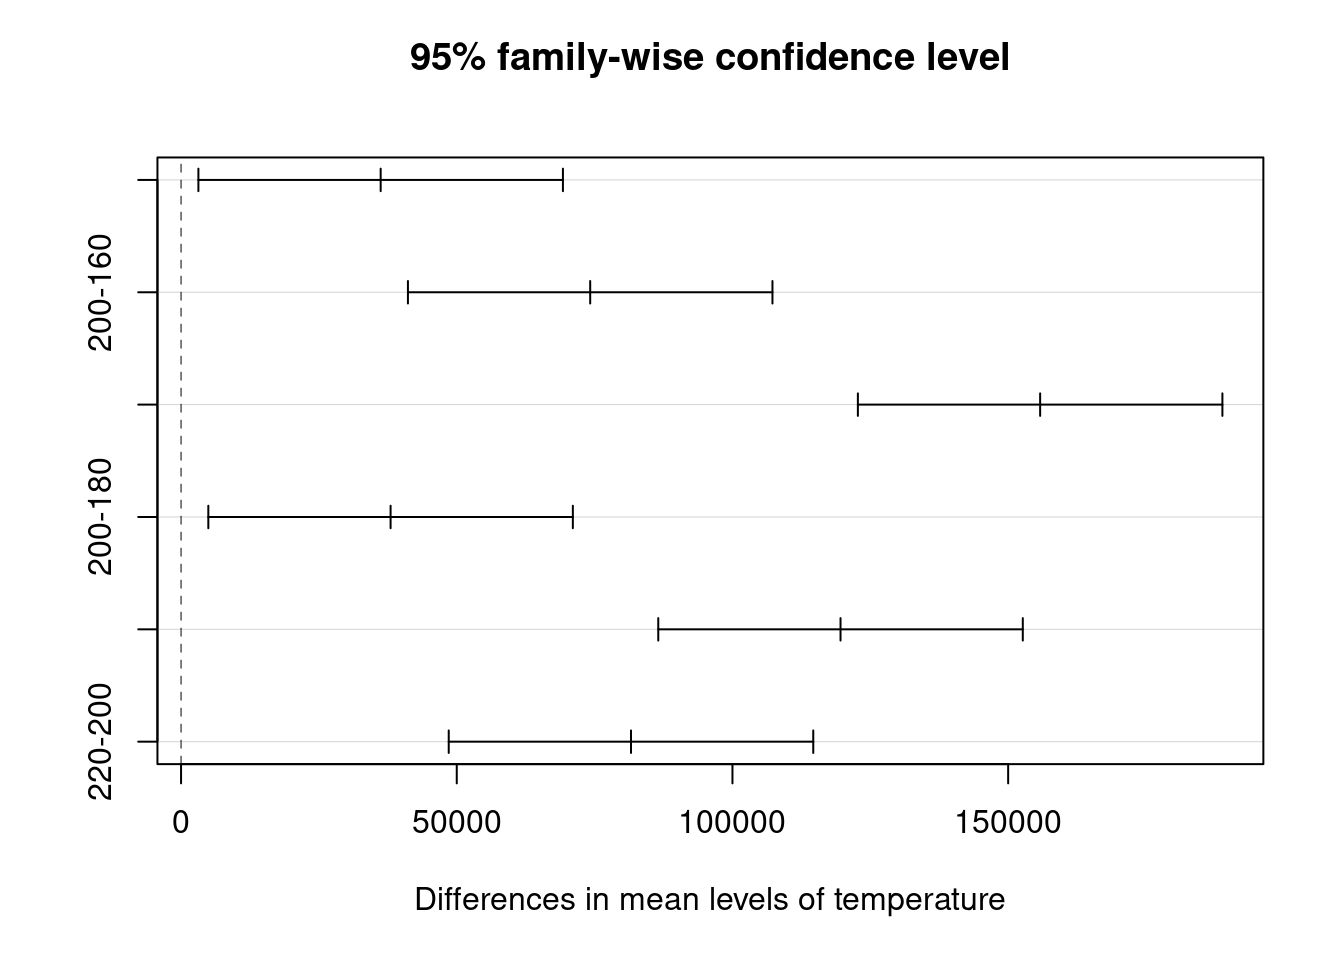
\includegraphics[width=0.8\linewidth]{two_means_comparison_files/figure-latex/unnamed-chunk-9-1}

Another way to better understanding the bond distributions is to plot a box plot. This type of plot is somehow like the histogram seen before but more compact when several groups are required to be plotted.

\begin{Shaded}
\begin{Highlighting}[]
\NormalTok{cement\_long }\SpecialCharTok{\%\textgreater{}\%} 
  \FunctionTok{ggplot}\NormalTok{(}\FunctionTok{aes}\NormalTok{(}\AttributeTok{x =}\NormalTok{ treatment, }\AttributeTok{y =}\NormalTok{ y, }\AttributeTok{fill =}\NormalTok{ treatment)) }\SpecialCharTok{+}
  \FunctionTok{geom\_boxplot}\NormalTok{(}\AttributeTok{width =} \FloatTok{0.3}\NormalTok{) }\SpecialCharTok{+}
  \FunctionTok{theme\_light}\NormalTok{() }\SpecialCharTok{+}
  \FunctionTok{theme}\NormalTok{(}\AttributeTok{legend.position =} \StringTok{"none"}\NormalTok{) }\SpecialCharTok{+}
  \FunctionTok{labs}\NormalTok{(}\AttributeTok{title =} \StringTok{"Cement mortar case study"}\NormalTok{,}
       \AttributeTok{subtitle =} \StringTok{"Raw data plot"}\NormalTok{,}
       \AttributeTok{x =} \StringTok{"Treatment"}\NormalTok{,}
       \AttributeTok{y =} \StringTok{"Bond strength"}\NormalTok{)}
\end{Highlighting}
\end{Shaded}

\includegraphics[width=0.8\linewidth]{two_means_comparison_files/figure-latex/unnamed-chunk-10-1}

We would like to understand if the treatment has an effect. Thus we want to compare the two population means. For that we use a t test using samples obtained independently and randomly. Before running the test we also have to check the normality of the samples distributions and equality of their variances.

To do these checks we're using the stat\_qq functions from the ggplot package and plotting the qq plots for both levels in the same plot:

\begin{Shaded}
\begin{Highlighting}[]
\NormalTok{cement\_long }\SpecialCharTok{\%\textgreater{}\%}
  \FunctionTok{ggplot}\NormalTok{(}\FunctionTok{aes}\NormalTok{(}\AttributeTok{sample =}\NormalTok{ y, }\AttributeTok{color =}\NormalTok{ treatment)) }\SpecialCharTok{+}
  \FunctionTok{geom\_qq}\NormalTok{() }\SpecialCharTok{+}
  \FunctionTok{geom\_qq\_line}\NormalTok{() }\SpecialCharTok{+}
  \FunctionTok{coord\_flip}\NormalTok{() }\SpecialCharTok{+}
  \FunctionTok{theme\_light}\NormalTok{() }\SpecialCharTok{+}
  \FunctionTok{labs}\NormalTok{(}\AttributeTok{title =} \StringTok{"Cement mortar case study"}\NormalTok{,}
       \AttributeTok{subtitle =} \StringTok{"Raw data plot"}\NormalTok{,}
       \AttributeTok{x =} \StringTok{"Treatment"}\NormalTok{,}
       \AttributeTok{y =} \StringTok{"Bond strength"}\NormalTok{)}
\end{Highlighting}
\end{Shaded}

\includegraphics[width=0.8\linewidth]{two_means_comparison_files/figure-latex/unnamed-chunk-11-1}

We observe that for both levels of treatment the data is adhering to the straight line thus we can assume they follow a normal distribution. Also both lines in the qq plot before have equivalent slopes indicating that the assumption of variances is a reasonable one. These verifications are summary ones. We review in subsequent sessions other deeper verifications of such as the shapiro-wilk normality test.

We're now going to apply the t-test:

\begin{Shaded}
\begin{Highlighting}[]
\FunctionTok{library}\NormalTok{(stats)}
\end{Highlighting}
\end{Shaded}

\begin{Shaded}
\begin{Highlighting}[]
\FunctionTok{t.test}\NormalTok{(y }\SpecialCharTok{\textasciitilde{}}\NormalTok{ treatment, }\AttributeTok{data =}\NormalTok{ cement\_long, }\AttributeTok{var.equal =} \ConstantTok{TRUE}\NormalTok{)}
\end{Highlighting}
\end{Shaded}

\begin{verbatim}
	Two Sample t-test

data:  y by treatment
t = -2.1869, df = 18, p-value = 0.0422
alternative hypothesis: true difference in means is not equal to 0
95 percent confidence interval:
 -0.54507339 -0.01092661
sample estimates:
  mean in group Modified mean in group Unmodified 
                  16.764                   17.042 
\end{verbatim}

We see that p \textless{} 0.05 thus the means differ significantly. Furthemore the mean difference is estimated with 95\% confidence, to be between -0.55 and -0.01 (to be noted that zero is obviously not included in this interval). There is an effect in our treatment that explains the difference in means between the two samples.

\hypertarget{t-test-two-samples-paired}{%
\subsubsection{t-test two samples paired}\label{t-test-two-samples-paired}}

\begin{Shaded}
\begin{Highlighting}[]
\NormalTok{hardness }\OtherTok{\textless{}{-}} \FunctionTok{read\_csv}\NormalTok{(}\StringTok{"../industRial/data{-}raw/2\_hardness.csv"}\NormalTok{)}
\FunctionTok{t.test}\NormalTok{(}\AttributeTok{x =}\NormalTok{ hardness}\SpecialCharTok{$}\NormalTok{Tip1, }\AttributeTok{y =}\NormalTok{ hardness}\SpecialCharTok{$}\NormalTok{Tip2, }\AttributeTok{paired =} \ConstantTok{TRUE}\NormalTok{)}
\end{Highlighting}
\end{Shaded}

\begin{verbatim}
	Paired t-test

data:  hardness$Tip1 and hardness$Tip2
t = -0.26414, df = 9, p-value = 0.7976
alternative hypothesis: true difference in means is not equal to 0
95 percent confidence interval:
 -0.9564389  0.7564389
sample estimates:
mean of the differences 
                   -0.1 
\end{verbatim}

p \textgreater{} 0.05 thus the means cannot be considered different (we cannot reject the null hypothesis) The mean difference is with 95\% confidence between -0.96 and 0.76.

Note that because it is paired although there are 20 measurements there are only 9 degrees of freedom (10 times the differences between the measurements, minus 1).

Randomization of the test sequence is a required practice, not only because of operator effects but also due to other potentially unknown effects like machine warm up.

\hypertarget{two-variances-comparison}{%
\subsection{Two variances comparison}\label{two-variances-comparison}}

Bonett's test is accurate for any continuous distribution and does not require that the data are normal. Bonett's test is usually more reliable than Levene's test.

Levene's test is also accurate with any continuous distribution. For extremely skewed and heavy tailed distributions, Levene's method tends to be more reliable than Bonett's method.

The F-test is accurate only for normally distributed data. Any small deviation from normality can cause the F-test to be inaccurate, even with large samples. However, if the data conform well to the normal distribution, then the F-test is usually more powerful than either Bonett's test or Levene's test.

\begin{Shaded}
\begin{Highlighting}[]
\FunctionTok{library}\NormalTok{(tidyverse)}
\FunctionTok{library}\NormalTok{(readxl)}
\FunctionTok{library}\NormalTok{(stats)}

\NormalTok{filter }\OtherTok{\textless{}{-}}\NormalTok{ dplyr}\SpecialCharTok{::}\NormalTok{filter}
\NormalTok{select }\OtherTok{\textless{}{-}}\NormalTok{ dplyr}\SpecialCharTok{::}\NormalTok{select}
\end{Highlighting}
\end{Shaded}

\hypertarget{bonetts-test}{%
\subsubsection{Bonett's test}\label{bonetts-test}}

\hypertarget{leveneTest}{%
\subsubsection{Levene test}\label{leveneTest}}

Homogeneity of variances test

You want test samples to see for homogeneity of variance (homoscedasticity)

\textbf{Data loading}

\begin{Shaded}
\begin{Highlighting}[]
\NormalTok{cement }\OtherTok{\textless{}{-}} \FunctionTok{read\_csv}\NormalTok{(}\StringTok{"../industRial/data{-}raw/2\_cement.csv"}\NormalTok{)}
\NormalTok{cement\_long }\OtherTok{\textless{}{-}}\NormalTok{ cement }\SpecialCharTok{\%\textgreater{}\%}
  \FunctionTok{pivot\_longer}\NormalTok{(}
    \AttributeTok{cols =} \FunctionTok{everything}\NormalTok{(), }\AttributeTok{names\_to =} \StringTok{"treatment"}\NormalTok{, }\AttributeTok{values\_to =} \StringTok{"y"}
\NormalTok{  )}
\end{Highlighting}
\end{Shaded}

\begin{Shaded}
\begin{Highlighting}[]
\FunctionTok{library}\NormalTok{(car)}
\end{Highlighting}
\end{Shaded}

\begin{Shaded}
\begin{Highlighting}[]
\FunctionTok{leveneTest}\NormalTok{(y }\SpecialCharTok{\textasciitilde{}}\NormalTok{ treatment, }\AttributeTok{data =}\NormalTok{ cement\_long)}
\end{Highlighting}
\end{Shaded}

\begin{verbatim}
Levene's Test for Homogeneity of Variance (center = median)
      Df F value Pr(>F)
group  1  1.9528 0.1793
      18               
\end{verbatim}

Pr \textgreater{} 0.05 thus there is homogeneity of the variances (they do not differ significantly).

\hypertarget{FTest}{%
\subsubsection{F-test}\label{FTest}}

We're now confirming this with a variance test from the stats package.

\begin{Shaded}
\begin{Highlighting}[]
\FunctionTok{var.test}\NormalTok{(y }\SpecialCharTok{\textasciitilde{}}\NormalTok{ treatment, cement\_long)}
\end{Highlighting}
\end{Shaded}

\begin{verbatim}
	F test to compare two variances

data:  y by treatment
F = 1.6293, num df = 9, denom df = 9, p-value = 0.4785
alternative hypothesis: true ratio of variances is not equal to 1
95 percent confidence interval:
 0.4046845 6.5593806
sample estimates:
ratio of variances 
          1.629257 
\end{verbatim}

The test null hypothesis is that the variances are equal. Since the p value is much greater than 0.05 we cannot reject the null hypotheses meaning that we can consider them equal.

In other words the probability that the variances are different is 47.85\% due to random cause.

\hypertarget{sample-size}{%
\subsection{Sample size}\label{sample-size}}

\begin{Shaded}
\begin{Highlighting}[]
\FunctionTok{library}\NormalTok{(tidyverse)}
\FunctionTok{library}\NormalTok{(readxl)}
\FunctionTok{library}\NormalTok{(stats)}

\NormalTok{filter }\OtherTok{\textless{}{-}}\NormalTok{ dplyr}\SpecialCharTok{::}\NormalTok{filter}
\NormalTok{select }\OtherTok{\textless{}{-}}\NormalTok{ dplyr}\SpecialCharTok{::}\NormalTok{select}
\end{Highlighting}
\end{Shaded}

\textbf{Data loading}

\begin{Shaded}
\begin{Highlighting}[]
\NormalTok{cement }\OtherTok{\textless{}{-}} \FunctionTok{read\_csv}\NormalTok{(}\StringTok{"../industRial/data{-}raw/2\_cement.csv"}\NormalTok{)}
\NormalTok{cement\_long }\OtherTok{\textless{}{-}}\NormalTok{ cement }\SpecialCharTok{\%\textgreater{}\%}
  \FunctionTok{pivot\_longer}\NormalTok{(}
    \AttributeTok{cols =} \FunctionTok{everything}\NormalTok{(), }\AttributeTok{names\_to =} \StringTok{"treatment"}\NormalTok{, }\AttributeTok{values\_to =} \StringTok{"y"}
\NormalTok{  )}
\end{Highlighting}
\end{Shaded}

\begin{Shaded}
\begin{Highlighting}[]
\CommentTok{\# Calculate the required sample size for a certain t{-}test power}
\NormalTok{cohen\_d }\OtherTok{\textless{}{-}} \FloatTok{0.27} \SpecialCharTok{/} \FloatTok{0.25} \CommentTok{\# Cohen\textquotesingle{}s effect size = difference of means / sd}
\CommentTok{\# A Cohen\textquotesingle{}s d of 2 means that the averages changed by 2 standard deviations, which is very large.}
\FunctionTok{power.t.test}\NormalTok{(}\AttributeTok{d =}\NormalTok{ cohen\_d, }\AttributeTok{power =} \FloatTok{0.95}\NormalTok{)}
\end{Highlighting}
\end{Shaded}

\begin{verbatim}
     Two-sample t test power calculation 

              n = 23.28802
          delta = 1.08
             sd = 1
      sig.level = 0.05
          power = 0.95
    alternative = two.sided

NOTE: n is number in *each* group
\end{verbatim}

\begin{Shaded}
\begin{Highlighting}[]
\FunctionTok{library}\NormalTok{(lsr)}
\end{Highlighting}
\end{Shaded}

\begin{Shaded}
\begin{Highlighting}[]
\CommentTok{\# By comparison, calculate Cohen\textquotesingle{}s d for the dataset}
\FunctionTok{cohensD}\NormalTok{(}\AttributeTok{x =}\NormalTok{ cement}\SpecialCharTok{$}\NormalTok{Modified, }\AttributeTok{y =}\NormalTok{ cement}\SpecialCharTok{$}\NormalTok{Unmodified)}
\end{Highlighting}
\end{Shaded}

\begin{verbatim}
[1] 0.9780006
\end{verbatim}

In this example if we wanted to detect a significant difference of at least 0.25 in the means with a probability of at least 95\% (Power of 0.95) we would need to use 8 (7.6) samples of each (to be)

\hypertarget{one-factor-multiple-levels}{%
\section{One factor multiple levels}\label{one-factor-multiple-levels}}

\hypertarget{linear-regression}{%
\subsection{Linear regression}\label{linear-regression}}

We will present here a first example of the utilisation of linear regression techniques and establish a linear model. These models are going to be used extensively in the upcoming cases.

\textbf{Plasma etching example}

\textbf{Data loading}

\begin{Shaded}
\begin{Highlighting}[]
\FunctionTok{library}\NormalTok{(tidyverse)}
\FunctionTok{library}\NormalTok{(janitor)}
\FunctionTok{library}\NormalTok{(stats)}
\FunctionTok{library}\NormalTok{(knitr)}
\NormalTok{filter }\OtherTok{\textless{}{-}}\NormalTok{ dplyr}\SpecialCharTok{::}\NormalTok{filter}
\NormalTok{select }\OtherTok{\textless{}{-}}\NormalTok{ dplyr}\SpecialCharTok{::}\NormalTok{select}
\end{Highlighting}
\end{Shaded}

\begin{Shaded}
\begin{Highlighting}[]
\CommentTok{\# Direct copy of the example from the book:}
\NormalTok{plasma }\OtherTok{\textless{}{-}} \FunctionTok{read\_csv}\NormalTok{(}\StringTok{"../industRial/data{-}raw/3{-}1\_plasma\_etching.csv"}\NormalTok{) }\SpecialCharTok{\%\textgreater{}\%}
  \FunctionTok{clean\_names}\NormalTok{()}

\NormalTok{plasma\_narrow }\OtherTok{\textless{}{-}}\NormalTok{ plasma }\SpecialCharTok{\%\textgreater{}\%}
  \FunctionTok{pivot\_longer}\NormalTok{(}
    \AttributeTok{cols =} \FunctionTok{starts\_with}\NormalTok{(}\StringTok{"x"}\NormalTok{),}
    \AttributeTok{names\_to =} \StringTok{"observation"}\NormalTok{,}
    \AttributeTok{values\_to =} \StringTok{"etch\_rate"}
\NormalTok{  )}
\end{Highlighting}
\end{Shaded}

\begin{Shaded}
\begin{Highlighting}[]
\FunctionTok{head}\NormalTok{(plasma\_narrow) }\SpecialCharTok{\%\textgreater{}\%} 
  \FunctionTok{kable}\NormalTok{(}\AttributeTok{align =} \StringTok{"c"}\NormalTok{, }
        \AttributeTok{caption =} \StringTok{"plasma etching experiment data"}\NormalTok{, }
        \AttributeTok{booktabs =}\NormalTok{ T)}
\end{Highlighting}
\end{Shaded}

\textbackslash begin\{table\}

\textbackslash caption\{(\#tab:tab-plasma\_narrow)plasma etching experiment data\}
\centering

\begin{tabular}[t]{ccc}
\toprule
power & observation & etch\_rate\\
\midrule
160 & x1 & 575\\
160 & x2 & 542\\
160 & x3 & 530\\
160 & x4 & 539\\
160 & x5 & 570\\
\addlinespace
180 & x1 & 565\\
\bottomrule
\end{tabular}

\textbackslash end\{table\}

\textbf{Raw data plot}

\begin{Shaded}
\begin{Highlighting}[]
\FunctionTok{ggplot}\NormalTok{(plasma\_narrow, }\FunctionTok{aes}\NormalTok{(}\AttributeTok{x =}\NormalTok{ power, }\AttributeTok{y =}\NormalTok{ etch\_rate)) }\SpecialCharTok{+}
  \FunctionTok{geom\_point}\NormalTok{() }\SpecialCharTok{+}
  \FunctionTok{theme\_light}\NormalTok{() }\SpecialCharTok{+}
  \FunctionTok{theme}\NormalTok{(}\AttributeTok{legend.position =} \StringTok{"none"}\NormalTok{) }\SpecialCharTok{+}
  \FunctionTok{labs}\NormalTok{(}\AttributeTok{title =} \StringTok{"Plasma case study"}\NormalTok{,}
       \AttributeTok{subtitle =} \StringTok{"Raw data plot"}\NormalTok{,}
       \AttributeTok{x =} \StringTok{"Power"}\NormalTok{,}
       \AttributeTok{y =} \StringTok{"Etch rate"}\NormalTok{)}
\end{Highlighting}
\end{Shaded}

\includegraphics[width=0.8\linewidth]{linear_regression_files/figure-latex/unnamed-chunk-4-1}

\hypertarget{linearModel}{%
\subsubsection{Linear model function}\label{linearModel}}

Here we're constructing a linear model of the raw data and not a model of the Anova, thus \emph{power} has to be as integer and not as a factor, unlike in the Anova model.

\begin{Shaded}
\begin{Highlighting}[]
\FunctionTok{library}\NormalTok{(stats)}
\end{Highlighting}
\end{Shaded}

\begin{Shaded}
\begin{Highlighting}[]
\NormalTok{plasma\_lm }\OtherTok{\textless{}{-}} \FunctionTok{lm}\NormalTok{(etch\_rate }\SpecialCharTok{\textasciitilde{}}\NormalTok{ power, }\AttributeTok{data =}\NormalTok{ plasma\_narrow)}
\FunctionTok{summary}\NormalTok{(plasma\_lm)}
\end{Highlighting}
\end{Shaded}

\begin{verbatim}
Call:
lm(formula = etch_rate ~ power, data = plasma_narrow)

Residuals:
   Min     1Q Median     3Q    Max 
-43.02 -12.32  -1.21  16.71  33.06 

Coefficients:
            Estimate Std. Error t value Pr(>|t|)    
(Intercept) 137.6200    41.2108   3.339  0.00365 ** 
power         2.5270     0.2154  11.731 7.26e-10 ***
---
Signif. codes:  0 '***' 0.001 '**' 0.01 '*' 0.05 '.' 0.1 ' ' 1

Residual standard error: 21.54 on 18 degrees of freedom
Multiple R-squared:  0.8843,	Adjusted R-squared:  0.8779 
F-statistic: 137.6 on 1 and 18 DF,  p-value: 7.263e-10
\end{verbatim}

\hypertarget{linear-model-plot}{%
\subsubsection{Linear model plot}\label{linear-model-plot}}

\begin{Shaded}
\begin{Highlighting}[]
\FunctionTok{ggplot}\NormalTok{(plasma\_narrow, }\FunctionTok{aes}\NormalTok{(}\AttributeTok{x =}\NormalTok{ power, }\AttributeTok{y =}\NormalTok{ etch\_rate)) }\SpecialCharTok{+}
  \FunctionTok{geom\_point}\NormalTok{() }\SpecialCharTok{+}
  \FunctionTok{geom\_smooth}\NormalTok{(}\AttributeTok{method =} \StringTok{"lm"}\NormalTok{) }\SpecialCharTok{+}
  \FunctionTok{theme\_light}\NormalTok{() }\SpecialCharTok{+}
  \FunctionTok{theme}\NormalTok{(}\AttributeTok{legend.position =} \StringTok{"none"}\NormalTok{) }\SpecialCharTok{+}
  \FunctionTok{labs}\NormalTok{(}\AttributeTok{title =} \StringTok{"Plasma case study"}\NormalTok{,}
       \AttributeTok{subtitle =} \StringTok{"Raw data plot"}\NormalTok{,}
       \AttributeTok{x =} \StringTok{"Power"}\NormalTok{,}
       \AttributeTok{y =} \StringTok{"Etch rate"}\NormalTok{)}
\end{Highlighting}
\end{Shaded}

\includegraphics[width=0.8\linewidth]{linear_regression_files/figure-latex/unnamed-chunk-7-1}

\hypertarget{linear-model-fixed-effects}{%
\subsubsection{Linear model fixed effects}\label{linear-model-fixed-effects}}

Reminder of fixed effects definition:

Fixed or Random Factor? The statistical model, Equation 3.2, describes two different situations with respect to the treatment effects. First, the a treatments could have been specifically chosen by the experimenter. In this situation, we wish to test hypotheses about the treatment means, and our conclusions will apply only to the factor levels considered in the analysis. The conclusions cannot be extended to similar treatments that were not explicitly considered. We may also wish to estimate the model parameters (\$, .i, !2). This is called the fixed effects model. Alternatively, the treatments could be a random sample from a larger population of treatments. In this situation, we should like to be able to extend the conclusions (which are based on the sample of treatments) to all treatments in the population,

\begin{Shaded}
\begin{Highlighting}[]
\NormalTok{plasma\_narrow\_factor }\OtherTok{\textless{}{-}}\NormalTok{ plasma\_narrow }\SpecialCharTok{\%\textgreater{}\%}
  \FunctionTok{mutate}\NormalTok{(}\AttributeTok{power =} \FunctionTok{as\_factor}\NormalTok{(power))}
\NormalTok{plasma\_lm\_factor }\OtherTok{\textless{}{-}} \FunctionTok{lm}\NormalTok{(etch\_rate }\SpecialCharTok{\textasciitilde{}}\NormalTok{ power, }\AttributeTok{data =}\NormalTok{ plasma\_narrow\_factor)}
\FunctionTok{summary}\NormalTok{(plasma\_lm\_factor)}
\end{Highlighting}
\end{Shaded}

\begin{verbatim}
Call:
lm(formula = etch_rate ~ power, data = plasma_narrow_factor)

Residuals:
   Min     1Q Median     3Q    Max 
 -25.4  -13.0    2.8   13.2   25.6 

Coefficients:
            Estimate Std. Error t value Pr(>|t|)    
(Intercept)  551.200      8.169  67.471  < 2e-16 ***
power180      36.200     11.553   3.133  0.00642 ** 
power200      74.200     11.553   6.422 8.44e-06 ***
power220     155.800     11.553  13.485 3.73e-10 ***
---
Signif. codes:  0 '***' 0.001 '**' 0.01 '*' 0.05 '.' 0.1 ' ' 1

Residual standard error: 18.27 on 16 degrees of freedom
Multiple R-squared:  0.9261,	Adjusted R-squared:  0.9122 
F-statistic:  66.8 on 3 and 16 DF,  p-value: 2.883e-09
\end{verbatim}

\hypertarget{model-check-residuals}{%
\subsection{Model check \& residuals}\label{model-check-residuals}}

In order to assess the model performance we're going to look into the residuals. R provides direct ploting functions with the base and stats packages but in this first example we're going to break down the analysis and further customise the plots. We are also going to make usage of some additional statistical tests to confirm our observations from the plots. In subsequent chapters we'll have a more selective approach on a needed basis.

We start by loading the package broom which will help us retrieving the data from the lm object into a data frame.

\begin{Shaded}
\begin{Highlighting}[]
\FunctionTok{library}\NormalTok{(broom)}
\end{Highlighting}
\end{Shaded}

Now we build and show below an extract of the ``augmented'' dataframe

\begin{Shaded}
\begin{Highlighting}[]
\NormalTok{plasma\_aug }\OtherTok{\textless{}{-}} \FunctionTok{augment}\NormalTok{(plasma\_lm\_factor) }\SpecialCharTok{\%\textgreater{}\%}
  \FunctionTok{mutate}\NormalTok{(}\AttributeTok{index =} \FunctionTok{row\_number}\NormalTok{())}
\NormalTok{plasma\_aug }\SpecialCharTok{\%\textgreater{}\%}
  \FunctionTok{head}\NormalTok{() }\SpecialCharTok{\%\textgreater{}\%}
  \FunctionTok{kable}\NormalTok{(}\AttributeTok{align =} \StringTok{"c"}\NormalTok{)}
\end{Highlighting}
\end{Shaded}

\begin{tabular}{c|c|c|c|c|c|c|c|c}
\hline
etch\_rate & power & .fitted & .resid & .std.resid & .hat & .sigma & .cooksd & index\\
\hline
575 & 160 & 551.2 & 23.8 & 1.4566455 & 0.2 & 17.57109 & 0.1326135 & 1\\
\hline
542 & 160 & 551.2 & -9.2 & -0.5630730 & 0.2 & 18.67869 & 0.0198157 & 2\\
\hline
530 & 160 & 551.2 & -21.2 & -1.2975161 & 0.2 & 17.84638 & 0.1052218 & 3\\
\hline
539 & 160 & 551.2 & -12.2 & -0.7466838 & 0.2 & 18.53492 & 0.0348460 & 4\\
\hline
570 & 160 & 551.2 & 18.8 & 1.1506275 & 0.2 & 18.06913 & 0.0827465 & 5\\
\hline
565 & 180 & 587.4 & -22.4 & -1.3709604 & 0.2 & 17.72381 & 0.1174708 & 6\\
\hline
\end{tabular}

We can see we've obtained detailed model parameters such us fitted values and residuals for each DOE run.

\hypertarget{time-sequence-plot}{%
\subsubsection{Time sequence plot}\label{time-sequence-plot}}

For this plot we need to ensure that the order of plotting in the x axis corresponds exactly to the original data collection order. This plot allows us to assess for strange patterns such as a tendency to have runs of positive of negative results which indicates that the independency assumption does not hold. If patterns emerge then there may be correlation in the residuals.

\begin{Shaded}
\begin{Highlighting}[]
\NormalTok{plasma\_aug }\SpecialCharTok{\%\textgreater{}\%}
  \FunctionTok{ggplot}\NormalTok{(}\FunctionTok{aes}\NormalTok{(}\AttributeTok{x =}\NormalTok{ index, }\AttributeTok{y =}\NormalTok{ .resid)) }\SpecialCharTok{+}
  \FunctionTok{geom\_point}\NormalTok{() }\SpecialCharTok{+}
  \FunctionTok{theme\_light}\NormalTok{() }\SpecialCharTok{+}
  \FunctionTok{labs}\NormalTok{(}
    \AttributeTok{title =} \StringTok{"Plasma etching case study"}\NormalTok{,}
    \AttributeTok{subtitle =} \StringTok{"Linear model {-} Residuals timeseries"}\NormalTok{,}
    \AttributeTok{y =} \StringTok{"Index"}\NormalTok{,}
    \AttributeTok{x =} \StringTok{"Fitted values"}\NormalTok{,}
    \AttributeTok{caption =} \StringTok{"Data source: D.Montgomery DOEs"}
\NormalTok{  )}
\end{Highlighting}
\end{Shaded}

\includegraphics[width=0.8\linewidth]{linear_regression_files/figure-latex/unnamed-chunk-11-1}

Nothing strange emerges from the current plot and the design shows as well randomised.

\hypertarget{residualsCorrelation}{%
\subsubsection{Autocorrelation test}\label{residualsCorrelation}}

It is always good to keep in mind that all visual observations can be complemented with a statistical test. In this case we're going to use the durbinWatson test from the car package (Companion to Applied Regression).

\begin{Shaded}
\begin{Highlighting}[]
\FunctionTok{library}\NormalTok{(car)}
\end{Highlighting}
\end{Shaded}

\begin{Shaded}
\begin{Highlighting}[]
\FunctionTok{durbinWatsonTest}\NormalTok{(plasma\_lm\_factor)}
\end{Highlighting}
\end{Shaded}

\begin{verbatim}
 lag Autocorrelation D-W Statistic p-value
   1      -0.5343347      2.960893   0.084
 Alternative hypothesis: rho != 0
\end{verbatim}

Although the output shows Autocorrelation of -0.53 we have to consider that the p value is greated than 0.05 thus there is not enough significance to say that there is autocorrelation.

\hypertarget{residuals-vs-fit-plot}{%
\subsubsection{Residuals vs fit plot}\label{residuals-vs-fit-plot}}

If the model is correct and the assumptions hold, the residuals should be structureless. In particular they should be unrelated to any other variable including the predicted response.

\begin{Shaded}
\begin{Highlighting}[]
\NormalTok{plasma\_aug }\SpecialCharTok{\%\textgreater{}\%}
  \FunctionTok{ggplot}\NormalTok{(}\FunctionTok{aes}\NormalTok{(}\AttributeTok{x =}\NormalTok{ .fitted, }\AttributeTok{y =}\NormalTok{ .resid)) }\SpecialCharTok{+}
  \FunctionTok{geom\_point}\NormalTok{() }\SpecialCharTok{+}
  \FunctionTok{theme\_light}\NormalTok{() }\SpecialCharTok{+}
  \FunctionTok{geom\_smooth}\NormalTok{(}\AttributeTok{method =} \StringTok{"loess"}\NormalTok{, }\AttributeTok{se =} \ConstantTok{FALSE}\NormalTok{, }\AttributeTok{color =} \StringTok{"red"}\NormalTok{) }\SpecialCharTok{+}
  \FunctionTok{labs}\NormalTok{(}
    \AttributeTok{title =} \StringTok{"Plasma etching case study"}\NormalTok{,}
    \AttributeTok{subtitle =} \StringTok{"Linear model {-} Residuals vs Fitted values"}\NormalTok{,}
    \AttributeTok{y =} \StringTok{"Residuals"}\NormalTok{,}
    \AttributeTok{x =} \StringTok{"Fitted values"}\NormalTok{,}
    \AttributeTok{caption =} \StringTok{"Data source: D.Montgomery DOEs"}
\NormalTok{  )}
\end{Highlighting}
\end{Shaded}

\includegraphics[width=0.8\linewidth]{linear_regression_files/figure-latex/unnamed-chunk-14-1}

In this plot we see no variance anomalies such as a higher variance for a certain factor level or other types of skweness.

\hypertarget{barlettTest}{%
\subsubsection{Equality of variance test}\label{barlettTest}}

In the plasma etch experiment, the normality assumption is not in question, so we can apply Bartlett's test to the etch rate data (Bartlett's test is very sensitive to the normality assumption). Consequently, when the validity of this assumption is doubtful, Bartlett's test should not be used and in this case use instead the Modified Levene test.

\begin{Shaded}
\begin{Highlighting}[]
\FunctionTok{bartlett.test}\NormalTok{(etch\_rate }\SpecialCharTok{\textasciitilde{}}\NormalTok{ power, }\AttributeTok{data =}\NormalTok{ plasma\_narrow\_factor)}
\end{Highlighting}
\end{Shaded}

\begin{verbatim}
	Bartlett test of homogeneity of variances

data:  etch_rate by power
Bartlett's K-squared = 0.43349, df = 3, p-value = 0.9332
\end{verbatim}

The P-value is P = 0.934, so we cannot reject the null hypothesis. There is no evidence to counter the claim that all five variances are the same. This is the same conclusion reached by analyzing the plot of residuals versus fitted values.

\hypertarget{normality-plot}{%
\subsubsection{Normality plot}\label{normality-plot}}

As the sample size is relatively small we're going to use a qq plot instead of an histogram to assess the normality of the residuals.

\begin{Shaded}
\begin{Highlighting}[]
\NormalTok{plasma\_aug }\SpecialCharTok{\%\textgreater{}\%}
  \FunctionTok{ggplot}\NormalTok{(}\FunctionTok{aes}\NormalTok{(}\AttributeTok{sample =}\NormalTok{ .resid)) }\SpecialCharTok{+}
  \FunctionTok{geom\_qq}\NormalTok{() }\SpecialCharTok{+}
  \FunctionTok{geom\_qq\_line}\NormalTok{() }\SpecialCharTok{+}
  \CommentTok{\# coord\_flip() +}
  \FunctionTok{theme\_light}\NormalTok{() }\SpecialCharTok{+}
  \FunctionTok{labs}\NormalTok{(}
    \AttributeTok{title =} \StringTok{"Plasma etching case study"}\NormalTok{,}
    \AttributeTok{subtitle =} \StringTok{"Linear model {-} qq plot"}\NormalTok{,}
    \AttributeTok{y =} \StringTok{"Residuals"}\NormalTok{,}
    \AttributeTok{x =} \StringTok{"Fitted values"}\NormalTok{,}
    \AttributeTok{caption =} \StringTok{"Data source: D.Montgomery DOEs"}
\NormalTok{  )}
\end{Highlighting}
\end{Shaded}

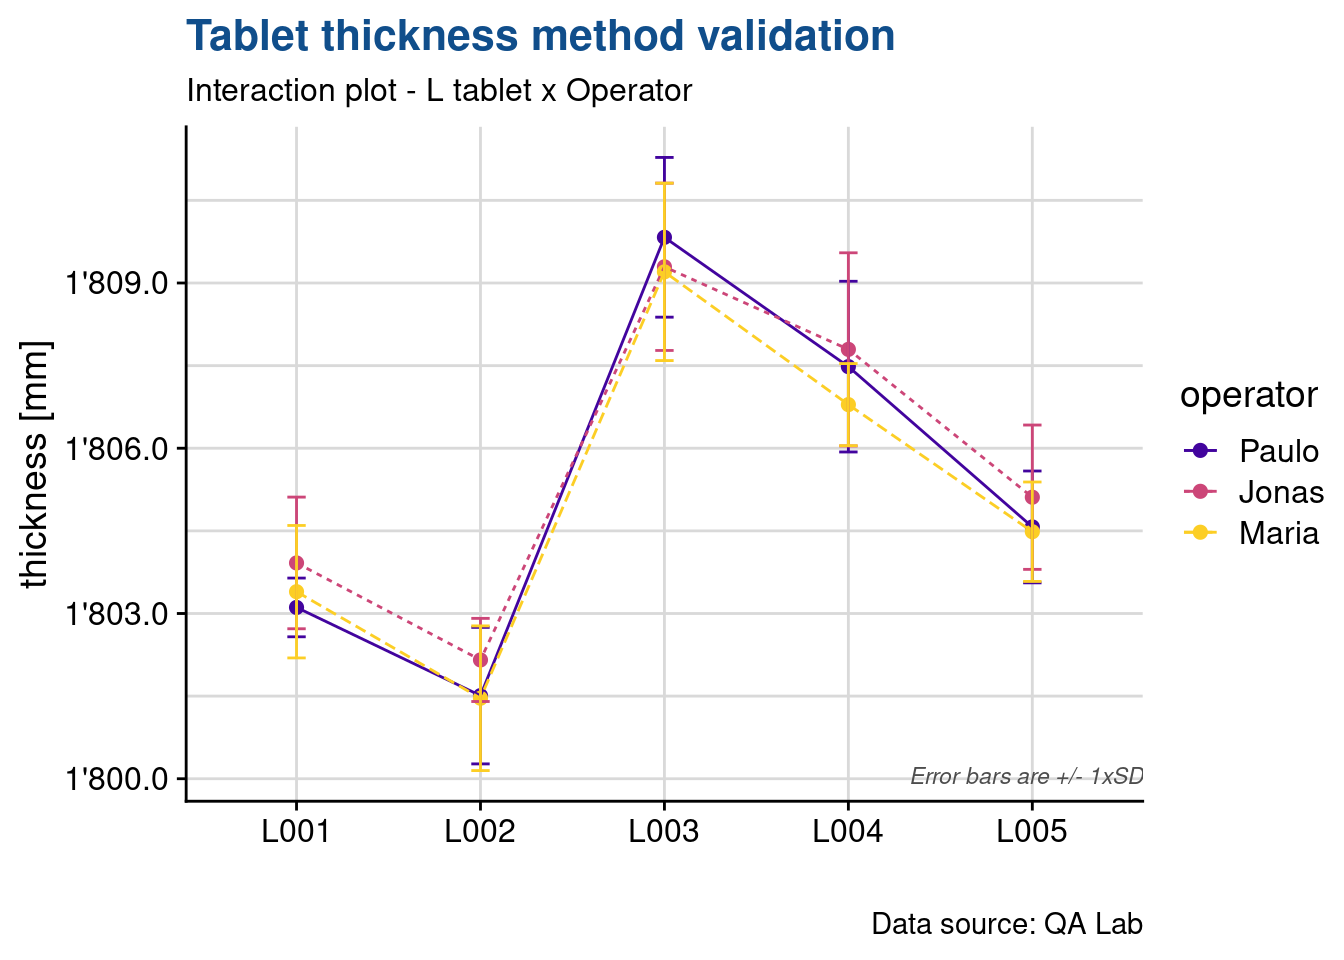
\includegraphics[width=0.8\linewidth]{linear_regression_files/figure-latex/unnamed-chunk-16-1}

The plot suggests normal distribution. We see that the error distribution is aproximately normal. In the fixed effects model we give more importance to the center of the values and here we consider acceptable that the extremes of the data tend to bend away from the straight line.
The verification can be completed by a test. For populations \textless{} 50 use the shapiro-wilk normality test.

\hypertarget{shapiroTest}{%
\subsubsection{Shapiro test}\label{shapiroTest}}

\begin{Shaded}
\begin{Highlighting}[]
\FunctionTok{shapiro.test}\NormalTok{(plasma\_aug}\SpecialCharTok{$}\NormalTok{.resid)}
\end{Highlighting}
\end{Shaded}

\begin{verbatim}
	Shapiro-Wilk normality test

data:  plasma_aug$.resid
W = 0.93752, p-value = 0.2152
\end{verbatim}

p \textgreater{} 0.05 indicates that the residuals do not differ significantly from a normally distributed population.

\hypertarget{std-residuals-vs-fit-plot}{%
\subsubsection{Std residuals vs fit plot}\label{std-residuals-vs-fit-plot}}

This specific Standardized residuals graph also help detecting outliers in the residuals (any residual \textgreater{} 3 standard deviations is a potential outlier).

\begin{Shaded}
\begin{Highlighting}[]
\NormalTok{plasma\_aug }\SpecialCharTok{\%\textgreater{}\%} 
  \FunctionTok{ggplot}\NormalTok{(}\FunctionTok{aes}\NormalTok{(}\AttributeTok{x =}\NormalTok{ .fitted, }\AttributeTok{y =}\NormalTok{ .std.resid)) }\SpecialCharTok{+}
  \FunctionTok{geom\_point}\NormalTok{() }\SpecialCharTok{+}
  \FunctionTok{theme\_light}\NormalTok{() }\SpecialCharTok{+}
  \FunctionTok{geom\_smooth}\NormalTok{(}\AttributeTok{method =} \StringTok{"loess"}\NormalTok{, }\AttributeTok{se =} \ConstantTok{FALSE}\NormalTok{, }\AttributeTok{color =} \StringTok{"red"}\NormalTok{) }\SpecialCharTok{+}
  \FunctionTok{labs}\NormalTok{(}\AttributeTok{title =} \StringTok{"Plasma etching case study"}\NormalTok{,}
       \AttributeTok{subtitle =} \StringTok{"Linear model {-} Standardised Residuals vs Fitted values"}\NormalTok{,}
       \AttributeTok{y =} \StringTok{"Standardised Residuals"}\NormalTok{,}
       \AttributeTok{x =} \StringTok{"Fitted values"}\NormalTok{,}
       \AttributeTok{caption =} \StringTok{"Data source: D.Montgomery DOEs"}\NormalTok{)}
\end{Highlighting}
\end{Shaded}

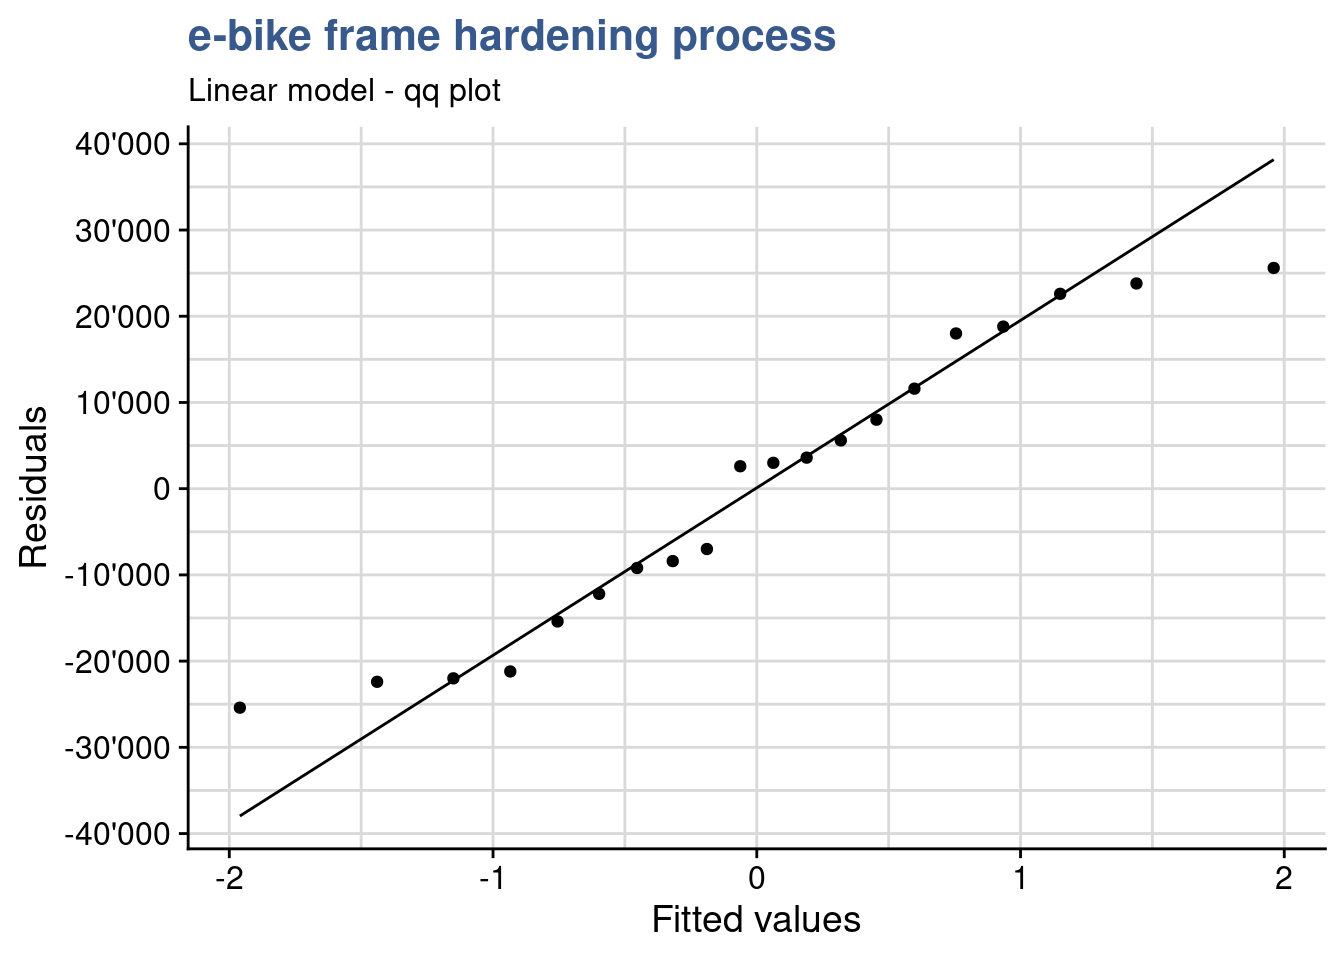
\includegraphics[width=0.8\linewidth]{linear_regression_files/figure-latex/unnamed-chunk-18-1}

The plot shows no outliers to consider in this DOE.

\hypertarget{outlierTest}{%
\subsubsection{Outlier test}\label{outlierTest}}

In a case where we were doubtfull we could go further and make a statistical test to assess if a certain value was an outlier. A usefull test is available in the car package.

\begin{Shaded}
\begin{Highlighting}[]
\FunctionTok{outlierTest}\NormalTok{(plasma\_lm\_factor)}
\end{Highlighting}
\end{Shaded}

\begin{verbatim}
No Studentized residuals with Bonferroni p < 0.05
Largest |rstudent|:
   rstudent unadjusted p-value Bonferroni p
12 1.648813            0.11997           NA
\end{verbatim}

In this case, the Bonferroni adjusted p value comes as NA confirming that there is no outlier in the data.

\hypertarget{cooks-distance-plot}{%
\subsubsection{Cooks distance plot}\label{cooks-distance-plot}}

\begin{Shaded}
\begin{Highlighting}[]
\NormalTok{plasma\_aug }\SpecialCharTok{\%\textgreater{}\%} 
  \FunctionTok{ggplot}\NormalTok{(}\FunctionTok{aes}\NormalTok{(}\AttributeTok{x =}\NormalTok{ .cooksd, }\AttributeTok{y =}\NormalTok{ .std.resid)) }\SpecialCharTok{+}
  \FunctionTok{geom\_point}\NormalTok{() }\SpecialCharTok{+}
  \FunctionTok{geom\_vline}\NormalTok{(}\AttributeTok{xintercept =} \FloatTok{0.5}\NormalTok{, }\AttributeTok{color =} \StringTok{"red"}\NormalTok{) }\SpecialCharTok{+}
  \FunctionTok{theme\_light}\NormalTok{() }\SpecialCharTok{+}
  \CommentTok{\# geom\_smooth(method = "glm", se = FALSE, color = "red") +}
  \FunctionTok{labs}\NormalTok{(}\AttributeTok{title =} \StringTok{"Plasma etching case study"}\NormalTok{,}
       \AttributeTok{subtitle =} \StringTok{"Pod L volume linear model {-} Residuals vs Leverage"}\NormalTok{,}
       \AttributeTok{y =} \StringTok{"Standardised Residuals"}\NormalTok{,}
       \AttributeTok{x =} \StringTok{"Cooks distance"}\NormalTok{,}
       \AttributeTok{caption =} \StringTok{"Data source: D.Montgomery DOEs"}\NormalTok{)}
\end{Highlighting}
\end{Shaded}

\includegraphics[width=0.8\linewidth]{linear_regression_files/figure-latex/unnamed-chunk-20-1}

\hypertarget{r-squared}{%
\subsubsection{R squared}\label{r-squared}}

R² the coefficient of determination

The R square can be extracted from the linear model that has been used to build the Anova model.

\begin{Shaded}
\begin{Highlighting}[]
\FunctionTok{summary}\NormalTok{(plasma\_lm\_factor)}\SpecialCharTok{$}\NormalTok{r.squared}
\end{Highlighting}
\end{Shaded}

\begin{verbatim}
[1] 0.9260598
\end{verbatim}

Thus, in the plasma etching experiment, the factor ``power'' explains about 88\% percent of the variability in etch rate.

Anova fixed effects assumes that:
- errors are normally distributed and are independent

As the number of residuals is too small we're not checking the normality via the histogram but rather with a a Q-Q plot.

\hypertarget{predict}{%
\subsection{Prediction}\label{predict}}

Here we're using the model with power as an integer:

\begin{Shaded}
\begin{Highlighting}[]
\NormalTok{power\_new }\OtherTok{\textless{}{-}} \FunctionTok{data.frame}\NormalTok{(}\AttributeTok{power =} \FunctionTok{c}\NormalTok{(}\DecValTok{170}\NormalTok{, }\DecValTok{190}\NormalTok{))}
\FunctionTok{predict}\NormalTok{(plasma\_lm, }\AttributeTok{newdata =}\NormalTok{ power\_new)}
\end{Highlighting}
\end{Shaded}

\begin{verbatim}
     1      2 
567.21 617.75 
\end{verbatim}

\hypertarget{multiple-means-comparison}{%
\subsection{Multiple means comparison}\label{multiple-means-comparison}}

\begin{Shaded}
\begin{Highlighting}[]
\FunctionTok{library}\NormalTok{(tidyverse)}
\FunctionTok{library}\NormalTok{(janitor)}
\FunctionTok{library}\NormalTok{(stats)}
\FunctionTok{library}\NormalTok{(knitr)}
\NormalTok{filter }\OtherTok{\textless{}{-}}\NormalTok{ dplyr}\SpecialCharTok{::}\NormalTok{filter}
\NormalTok{select }\OtherTok{\textless{}{-}}\NormalTok{ dplyr}\SpecialCharTok{::}\NormalTok{select}
\end{Highlighting}
\end{Shaded}

\begin{Shaded}
\begin{Highlighting}[]
\NormalTok{plasma }\OtherTok{\textless{}{-}} \FunctionTok{read\_csv}\NormalTok{(}\StringTok{"../industRial/data{-}raw/3{-}1\_plasma\_etching.csv"}\NormalTok{) }\SpecialCharTok{\%\textgreater{}\%}
  \FunctionTok{clean\_names}\NormalTok{()}

\NormalTok{plasma\_narrow }\OtherTok{\textless{}{-}}\NormalTok{ plasma }\SpecialCharTok{\%\textgreater{}\%}
  \FunctionTok{pivot\_longer}\NormalTok{(}
    \AttributeTok{cols =} \FunctionTok{starts\_with}\NormalTok{(}\StringTok{"x"}\NormalTok{),}
    \AttributeTok{names\_to =} \StringTok{"observation"}\NormalTok{,}
    \AttributeTok{values\_to =} \StringTok{"etch\_rate"}
\NormalTok{  )}
\end{Highlighting}
\end{Shaded}

\begin{Shaded}
\begin{Highlighting}[]
\NormalTok{plasma\_narrow\_factor }\OtherTok{\textless{}{-}}\NormalTok{ plasma\_narrow }\SpecialCharTok{\%\textgreater{}\%}
  \FunctionTok{mutate}\NormalTok{(}\AttributeTok{power =} \FunctionTok{as\_factor}\NormalTok{(power))}
\end{Highlighting}
\end{Shaded}

\hypertarget{box-plot-of-raw-data}{%
\subsubsection{Box plot of raw data}\label{box-plot-of-raw-data}}

We can also compare medians and get a sense of the effect of the treatment levels by looking into the box plot:

\begin{Shaded}
\begin{Highlighting}[]
\CommentTok{\# Box plot}
\FunctionTok{ggplot}\NormalTok{(plasma\_narrow\_factor, }\FunctionTok{aes}\NormalTok{(}\AttributeTok{x =}\NormalTok{ power, }\AttributeTok{y =}\NormalTok{ etch\_rate)) }\SpecialCharTok{+}
  \FunctionTok{geom\_boxplot}\NormalTok{() }\SpecialCharTok{+}
  \FunctionTok{theme\_light}\NormalTok{() }\SpecialCharTok{+}
  \FunctionTok{scale\_y\_continuous}\NormalTok{(}\AttributeTok{n.breaks =} \DecValTok{20}\NormalTok{) }\SpecialCharTok{+}
  \FunctionTok{theme}\NormalTok{(}\AttributeTok{legend.position =} \StringTok{"none"}\NormalTok{) }\SpecialCharTok{+}
  \FunctionTok{labs}\NormalTok{(}\AttributeTok{title =} \StringTok{"Plasma case study"}\NormalTok{,}
       \AttributeTok{subtitle =} \StringTok{"Raw data plot"}\NormalTok{,}
       \AttributeTok{x =} \StringTok{"Power"}\NormalTok{,}
       \AttributeTok{y =} \StringTok{"Etch rate"}\NormalTok{)}
\end{Highlighting}
\end{Shaded}

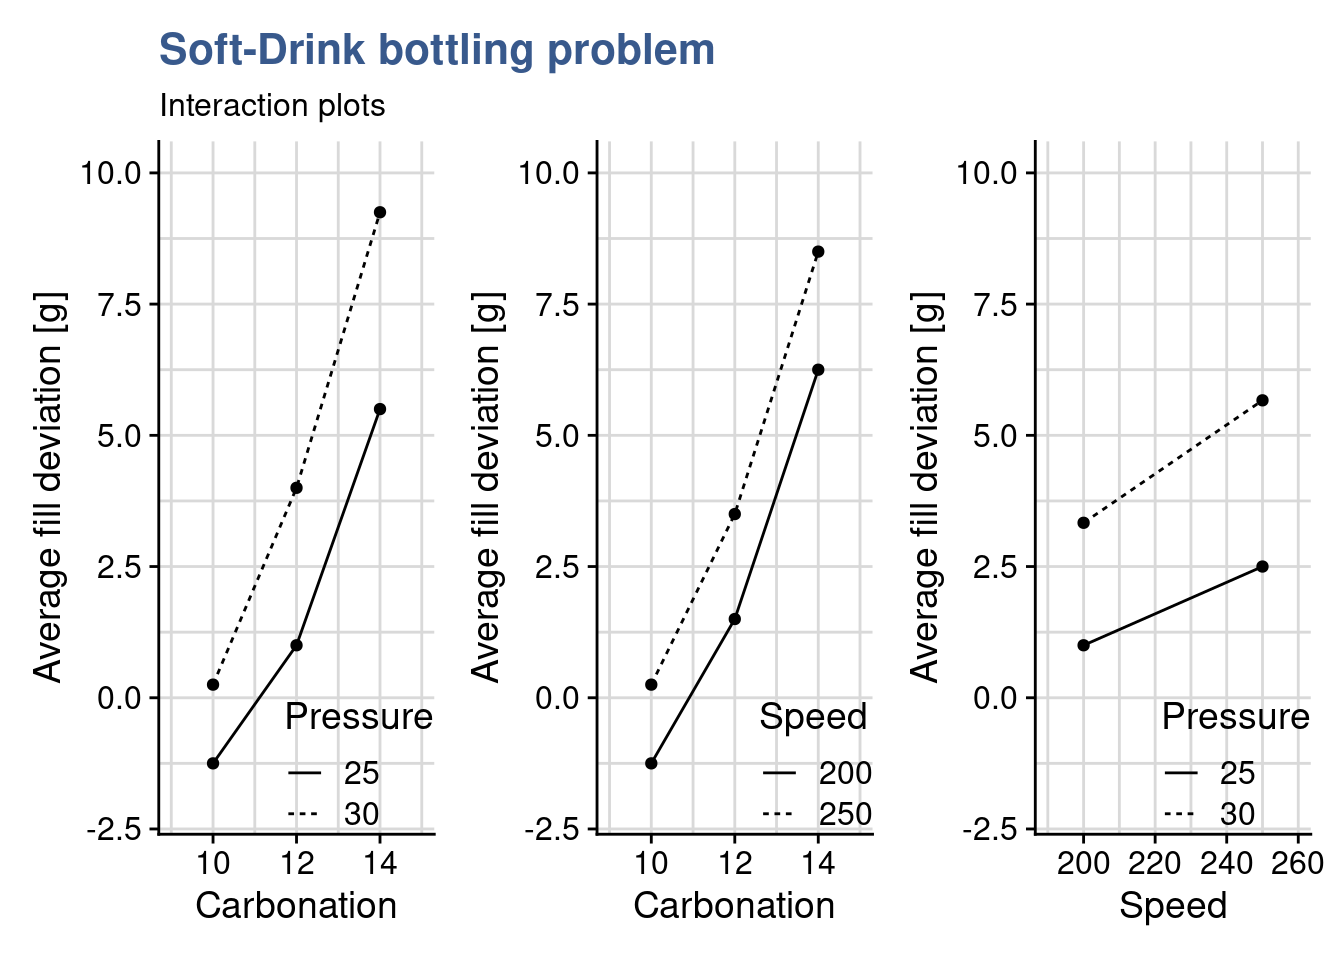
\includegraphics[width=0.8\linewidth]{anova_files/figure-latex/unnamed-chunk-5-1}

1 factor with severals levels + 1 continuous dependent variable
Similar to the t-test but extended - this test allows to compare the means between several levels of treatement for a continuous response variable (the t test is only 2 levels at a time, performing all pair wise t-tests would also not be a solution because its a lot of effort and would increase the type I error)

ANOVA principle: the total variability in the data, as measured by the total corrected sum of squares, can be partitioned into a sum of squares of the differences between the treatment averages and the grand average plus a sum of squares of the differences of observations within treatments from the treatment average

\hypertarget{anova}{%
\subsubsection{Anova with effect}\label{anova}}

In R the anova is built by passing the linear model to the anova or aov functions.
The output of the anova function is just the anova table as shown here for this first example. The output of the aov function is a list.

\begin{Shaded}
\begin{Highlighting}[]
\NormalTok{plasma\_lm\_factor }\OtherTok{\textless{}{-}} \FunctionTok{lm}\NormalTok{(etch\_rate }\SpecialCharTok{\textasciitilde{}}\NormalTok{ power, }\AttributeTok{data =}\NormalTok{ plasma\_narrow\_factor)}
\NormalTok{plasma\_aov }\OtherTok{\textless{}{-}} \FunctionTok{aov}\NormalTok{(plasma\_lm\_factor)}
\FunctionTok{summary}\NormalTok{(plasma\_aov)}
\end{Highlighting}
\end{Shaded}

\begin{verbatim}
            Df Sum Sq Mean Sq F value   Pr(>F)    
power        3  66871   22290    66.8 2.88e-09 ***
Residuals   16   5339     334                     
---
Signif. codes:  0 '***' 0.001 '**' 0.01 '*' 0.05 '.' 0.1 ' ' 1
\end{verbatim}

Note that the RF power or between-treatment mean square (22,290.18) is many times larger than the within-treatment or error mean square (333.70). This indicates that it is unlikely that the treatment means are equal.
Also p \textless{} 0.05 thus we can reject the null hypothesis and conclude that the means are significantly different.

\hypertarget{anova-with-no-effect}{%
\subsubsection{Anova with no effect}\label{anova-with-no-effect}}

Anova on plasma etching, modification of the example to achieve a p \textgreater{} 0.05:

\begin{Shaded}
\begin{Highlighting}[]
\NormalTok{plasma2 }\OtherTok{\textless{}{-}} \FunctionTok{read\_csv}\NormalTok{(}\StringTok{"../industRial/data{-}raw/3{-}1\_plasma\_etching\_2.csv"}\NormalTok{) }\SpecialCharTok{\%\textgreater{}\%}
  \FunctionTok{clean\_names}\NormalTok{()}

\NormalTok{plasma2\_narrow }\OtherTok{\textless{}{-}} \FunctionTok{gather}\NormalTok{(plasma2, }
\NormalTok{                         observation, }
\NormalTok{                         etch\_rate, x1, x2, x3, x4, x5)}
\NormalTok{plasma2\_narrow\_factor }\OtherTok{\textless{}{-}}\NormalTok{ plasma2\_narrow}
\NormalTok{plasma2\_narrow\_factor}\SpecialCharTok{$}\NormalTok{power }\OtherTok{\textless{}{-}} \FunctionTok{as.factor}\NormalTok{(plasma2\_narrow\_factor}\SpecialCharTok{$}\NormalTok{power)}

\NormalTok{plasma2\_lm\_factor }\OtherTok{\textless{}{-}} \FunctionTok{lm}\NormalTok{(etch\_rate }\SpecialCharTok{\textasciitilde{}}\NormalTok{ power, }\AttributeTok{data =}\NormalTok{ plasma2\_narrow\_factor)}
\FunctionTok{anova}\NormalTok{(plasma2\_lm\_factor)}
\end{Highlighting}
\end{Shaded}

\begin{verbatim}
Analysis of Variance Table

Response: etch_rate
          Df Sum Sq Mean Sq F value Pr(>F)
power      3   1476   492.0  1.2015  0.341
Residuals 16   6552   409.5               
\end{verbatim}

\begin{Shaded}
\begin{Highlighting}[]
\FunctionTok{ggplot}\NormalTok{(plasma2\_narrow\_factor, }\FunctionTok{aes}\NormalTok{(}\AttributeTok{x =}\NormalTok{ power, }\AttributeTok{y =}\NormalTok{ etch\_rate)) }\SpecialCharTok{+}
  \FunctionTok{geom\_boxplot}\NormalTok{() }\SpecialCharTok{+}
  \FunctionTok{theme\_light}\NormalTok{() }\SpecialCharTok{+}
  \FunctionTok{theme}\NormalTok{(}\AttributeTok{legend.position =} \StringTok{"none"}\NormalTok{) }\SpecialCharTok{+}
  \FunctionTok{labs}\NormalTok{(}\AttributeTok{title =} \StringTok{"Plasma case study"}\NormalTok{,}
       \AttributeTok{subtitle =} \StringTok{"Raw data plot"}\NormalTok{,}
       \AttributeTok{x =} \StringTok{"Power"}\NormalTok{,}
       \AttributeTok{y =} \StringTok{"Etch rate"}\NormalTok{)}
\end{Highlighting}
\end{Shaded}

\includegraphics[width=0.8\linewidth]{anova_files/figure-latex/unnamed-chunk-8-1}

P \textgreater{} 0.05 - there is no significant difference between the means

\hypertarget{pairwise-comparisons}{%
\subsection{Pairwise comparisons}\label{pairwise-comparisons}}

\hypertarget{tukeyTest}{%
\subsubsection{Tukey's test}\label{tukeyTest}}

The Anova may indicate that the treament means differ but it won't indicate which ones. In this case we may want to compare pairs of means.

\begin{Shaded}
\begin{Highlighting}[]
\NormalTok{plasma\_tukey }\OtherTok{\textless{}{-}} \FunctionTok{TukeyHSD}\NormalTok{(plasma\_aov, }\AttributeTok{ordered =} \ConstantTok{TRUE}\NormalTok{)}
\end{Highlighting}
\end{Shaded}

\begin{Shaded}
\begin{Highlighting}[]
\FunctionTok{head}\NormalTok{(plasma\_tukey}\SpecialCharTok{$}\NormalTok{power) }\SpecialCharTok{\%\textgreater{}\%} 
  \FunctionTok{kable}\NormalTok{(}\AttributeTok{align =} \StringTok{"c"}\NormalTok{, }
        \AttributeTok{caption =} \StringTok{"tukey test on plasma experiment"}\NormalTok{, }
        \AttributeTok{booktabs =}\NormalTok{ T)}
\end{Highlighting}
\end{Shaded}

\begin{table}

\caption{\label{tab:tab-plasmatukey}tukey test on plasma experiment}
\centering
\begin{tabular}[t]{lcccc}
\toprule
  & diff & lwr & upr & p adj\\
\midrule
180-160 & 36.2 & 3.145624 & 69.25438 & 0.0294279\\
200-160 & 74.2 & 41.145624 & 107.25438 & 0.0000455\\
220-160 & 155.8 & 122.745624 & 188.85438 & 0.0000000\\
200-180 & 38.0 & 4.945624 & 71.05438 & 0.0215995\\
220-180 & 119.6 & 86.545624 & 152.65438 & 0.0000001\\
\addlinespace
220-200 & 81.6 & 48.545624 & 114.65438 & 0.0000146\\
\bottomrule
\end{tabular}
\end{table}

The test provides us a simple direct calculation of the differences between the treatment means and a confidence interval for those. Most importantly it provides us with the p value to help us confirm the significance of the difference and conclude factor level by factor level which differences are significant.

Additionally we can obtain the related plot with the confidence intervals

\begin{Shaded}
\begin{Highlighting}[]
\FunctionTok{plot}\NormalTok{(plasma\_tukey)}
\end{Highlighting}
\end{Shaded}

\includegraphics[width=0.8\linewidth]{anova_files/figure-latex/unnamed-chunk-10-1}

\hypertarget{fisherLSD}{%
\subsubsection{Fisher's LSD}\label{fisherLSD}}

Fisher's Least Significant difference is an alternative to Tuckey's test.

\begin{Shaded}
\begin{Highlighting}[]
\FunctionTok{library}\NormalTok{(agricolae)}
\end{Highlighting}
\end{Shaded}

\begin{Shaded}
\begin{Highlighting}[]
\NormalTok{plasma\_anova }\OtherTok{\textless{}{-}} \FunctionTok{anova}\NormalTok{(plasma\_lm\_factor) }

\NormalTok{plasma\_LSD }\OtherTok{\textless{}{-}} \FunctionTok{LSD.test}\NormalTok{(}\AttributeTok{y =}\NormalTok{ plasma\_narrow\_factor}\SpecialCharTok{$}\NormalTok{etch\_rate,}
         \AttributeTok{trt =}\NormalTok{ plasma\_narrow\_factor}\SpecialCharTok{$}\NormalTok{power,}
         \AttributeTok{DFerror =}\NormalTok{ plasma\_anova}\SpecialCharTok{$}\NormalTok{Df[}\DecValTok{2}\NormalTok{],  }
         \AttributeTok{MSerror =}\NormalTok{ plasma\_anova}\SpecialCharTok{$}\StringTok{\textasciigrave{}}\AttributeTok{Mean Sq}\StringTok{\textasciigrave{}}\NormalTok{[}\DecValTok{2}\NormalTok{],}
         \AttributeTok{alpha =} \FloatTok{0.05}\NormalTok{)}
\end{Highlighting}
\end{Shaded}

The Fisher procedure provides us with many new additional information. A first outcome is the difference between means that can be considered significant, indicated in the table below by LSD = 24.49.

\begin{Shaded}
\begin{Highlighting}[]
\FunctionTok{head}\NormalTok{(plasma\_LSD}\SpecialCharTok{$}\NormalTok{statistics) }\SpecialCharTok{\%\textgreater{}\%} 
  \FunctionTok{kable}\NormalTok{(}\AttributeTok{align =} \StringTok{"c"}\NormalTok{, }
        \AttributeTok{caption =} \StringTok{"Fisher LSD procedure on plasma experiment: stats"}\NormalTok{, }
        \AttributeTok{booktabs =}\NormalTok{ T)}
\end{Highlighting}
\end{Shaded}

\begin{table}

\caption{\label{tab:tab-plasmafisherstatistics}Fisher LSD procedure on plasma experiment: stats}
\centering
\begin{tabular}[t]{lcccccc}
\toprule
  & MSerror & Df & Mean & CV & t.value & LSD\\
\midrule
 & 333.7 & 16 & 617.75 & 2.957095 & 2.119905 & 24.49202\\
\bottomrule
\end{tabular}
\end{table}

Furthermore it gives us a confidence interval for each treatment level mean:

\begin{Shaded}
\begin{Highlighting}[]
\FunctionTok{head}\NormalTok{(plasma\_LSD}\SpecialCharTok{$}\NormalTok{means) }\SpecialCharTok{\%\textgreater{}\%} 
  \CommentTok{\# as\_tibble() \%\textgreater{}\%}
  \FunctionTok{rename}\NormalTok{(}\AttributeTok{etch\_rate =} \StringTok{\textasciigrave{}}\AttributeTok{plasma\_narrow\_factor$etch\_rate}\StringTok{\textasciigrave{}}\NormalTok{) }\SpecialCharTok{\%\textgreater{}\%}
  \FunctionTok{select}\NormalTok{(}\SpecialCharTok{{-}}\NormalTok{Min, }\SpecialCharTok{{-}}\NormalTok{Max, }\SpecialCharTok{{-}}\NormalTok{Q25, }\SpecialCharTok{{-}}\NormalTok{Q50, }\SpecialCharTok{{-}}\NormalTok{Q75) }\SpecialCharTok{\%\textgreater{}\%}
  \FunctionTok{kable}\NormalTok{(}\AttributeTok{align =} \StringTok{"c"}\NormalTok{, }
        \AttributeTok{caption =} \StringTok{"Fisher LSD procedure on plasma experiment: means"}\NormalTok{, }
        \AttributeTok{booktabs =}\NormalTok{ T)}
\end{Highlighting}
\end{Shaded}

\begin{table}

\caption{\label{tab:tab-plasmafishermeans}Fisher LSD procedure on plasma experiment: means}
\centering
\begin{tabular}[t]{lccccc}
\toprule
  & etch\_rate & std & r & LCL & UCL\\
\midrule
160 & 551.2 & 20.01749 & 5 & 533.8815 & 568.5185\\
180 & 587.4 & 16.74216 & 5 & 570.0815 & 604.7185\\
200 & 625.4 & 20.52559 & 5 & 608.0815 & 642.7185\\
220 & 707.0 & 15.24795 & 5 & 689.6815 & 724.3185\\
\bottomrule
\end{tabular}
\end{table}

We can see for example that for power 220 W the etch rate if on average 707.0 with a probability of 95\% of being between 689.7 and 724.3 A/min.

Another interesting outcome is the grouping of levels for each factor:

\begin{Shaded}
\begin{Highlighting}[]
\FunctionTok{head}\NormalTok{(plasma\_LSD}\SpecialCharTok{$}\NormalTok{groups) }\SpecialCharTok{\%\textgreater{}\%} 
  \FunctionTok{kable}\NormalTok{(}\AttributeTok{align =} \StringTok{"c"}\NormalTok{, }
        \AttributeTok{caption =} \StringTok{"Fisher LSD procedure on plasma experiment: groups"}\NormalTok{, }
        \AttributeTok{booktabs =}\NormalTok{ T)}
\end{Highlighting}
\end{Shaded}

\begin{table}

\caption{\label{tab:tab-plasmafishergroups}Fisher LSD procedure on plasma experiment: groups}
\centering
\begin{tabular}[t]{lcc}
\toprule
  & plasma\_narrow\_factor\$etch\_rate & groups\\
\midrule
220 & 707.0 & a\\
200 & 625.4 & b\\
180 & 587.4 & c\\
160 & 551.2 & d\\
\bottomrule
\end{tabular}
\end{table}

In this case as all level means are statistically different they all show up in separate groups, each indicated by a specific letter.

Finally we can get from this package a plot with the Least significant difference error bars:

\begin{Shaded}
\begin{Highlighting}[]
\FunctionTok{plot}\NormalTok{(plasma\_LSD)}
\end{Highlighting}
\end{Shaded}

\includegraphics[width=0.8\linewidth]{anova_files/figure-latex/unnamed-chunk-13-1}

And below we're exploring a manual execution of this type of plot (in this case with the standard deviations instead).

\begin{Shaded}
\begin{Highlighting}[]
\FunctionTok{library}\NormalTok{(scales)}
\end{Highlighting}
\end{Shaded}

\begin{Shaded}
\begin{Highlighting}[]
\NormalTok{plasma\_narrow\_factor }\SpecialCharTok{\%\textgreater{}\%}
  \FunctionTok{group\_by}\NormalTok{(power) }\SpecialCharTok{\%\textgreater{}\%}
  \FunctionTok{summarise}\NormalTok{(}\AttributeTok{etch\_mean =} \FunctionTok{mean}\NormalTok{(etch\_rate), }\AttributeTok{etch\_sd =} \FunctionTok{sd}\NormalTok{(etch\_rate)) }\SpecialCharTok{\%\textgreater{}\%}
  \FunctionTok{ggplot}\NormalTok{(}\FunctionTok{aes}\NormalTok{(}\AttributeTok{x =}\NormalTok{ power, }\AttributeTok{y =}\NormalTok{ etch\_mean)) }\SpecialCharTok{+}
  \FunctionTok{geom\_point}\NormalTok{(}\AttributeTok{size =} \DecValTok{2}\NormalTok{) }\SpecialCharTok{+}
  \FunctionTok{geom\_line}\NormalTok{() }\SpecialCharTok{+}
  \FunctionTok{geom\_errorbar}\NormalTok{(}\FunctionTok{aes}\NormalTok{(}\AttributeTok{ymin =}\NormalTok{ etch\_mean }\SpecialCharTok{{-}}\NormalTok{ etch\_sd, }
                    \AttributeTok{ymax =}\NormalTok{ etch\_mean }\SpecialCharTok{+}\NormalTok{ etch\_sd),}
                \AttributeTok{width =}\NormalTok{ .}\DecValTok{1}\NormalTok{) }\SpecialCharTok{+}
  \CommentTok{\# scale\_y\_continuous(breaks = seq(10000, 20000, 10),}
  \CommentTok{\#                    labels = label\_number(big.mark = "\textquotesingle{}")) +}
  \CommentTok{\# scale\_color\_viridis\_d(option = "C", begin = 0.1, end = 0.9) +}
  \CommentTok{\# coord\_cartesian(ylim = c(17950, 18150)) +}
  \FunctionTok{annotate}\NormalTok{(}\AttributeTok{geom =} \StringTok{"text"}\NormalTok{, }\AttributeTok{x =} \ConstantTok{Inf}\NormalTok{, }\AttributeTok{y =} \SpecialCharTok{{-}}\ConstantTok{Inf}\NormalTok{, }\AttributeTok{label =} \StringTok{"Error bars are +/{-} 1xSD"}\NormalTok{, }
    \AttributeTok{hjust =} \DecValTok{1}\NormalTok{, }\AttributeTok{vjust =} \SpecialCharTok{{-}}\DecValTok{1}\NormalTok{, }\AttributeTok{colour =} \StringTok{"grey30"}\NormalTok{, }\AttributeTok{size =} \DecValTok{3}\NormalTok{, }
    \AttributeTok{fontface =} \StringTok{"italic"}\NormalTok{) }\SpecialCharTok{+}
  \FunctionTok{theme\_light}\NormalTok{() }\SpecialCharTok{+}
  \FunctionTok{labs}\NormalTok{(}\AttributeTok{title =} \StringTok{"axis volume method validation"}\NormalTok{,}
       \AttributeTok{subtitle =} \StringTok{"Interaction plot {-} L axis x Operator"}\NormalTok{,}
       \AttributeTok{x =} \StringTok{""}\NormalTok{,}
       \AttributeTok{y =} \StringTok{"Volume [mm]"}\NormalTok{,}
       \AttributeTok{caption =} \StringTok{"Data source: QA Lab"}\NormalTok{)}
\end{Highlighting}
\end{Shaded}

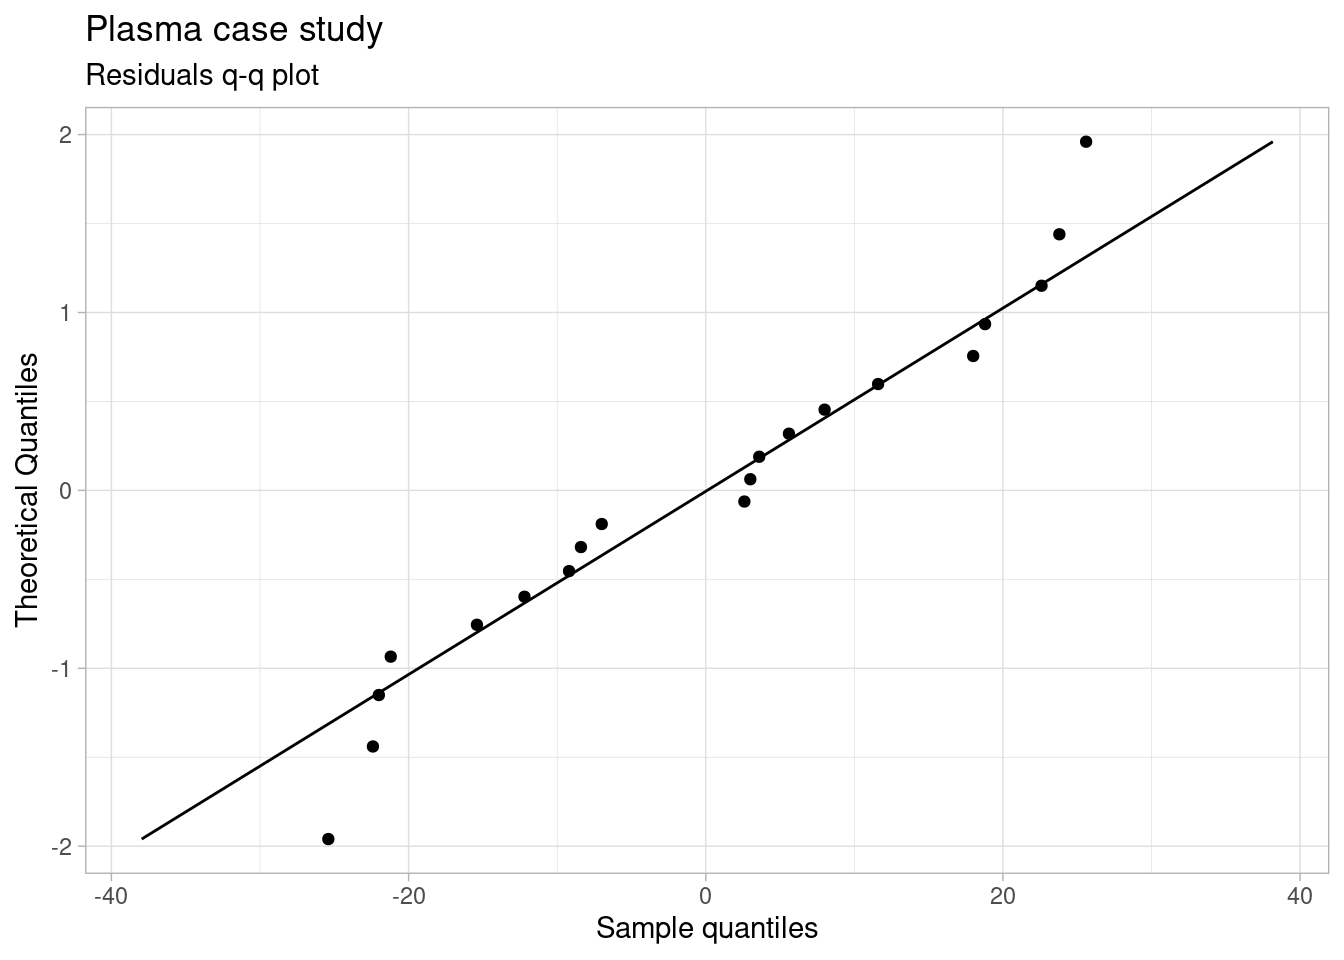
\includegraphics[width=0.8\linewidth]{anova_files/figure-latex/unnamed-chunk-15-1}

As there is no general consensus on which approach to use we recommend combine the Tukey test with the Fisher's LSD as completementary R functions. The Tukey test giving a first indication of the levels that have an effect and calculating the means differences and the Fisher function to provide much more additional information on each level. To be considered in each situation the slight difference between the significance level for difference between means and to decide if required to take the most conservative one.

\hypertarget{means-comparison-covariance}{%
\subsection{Means comparison \& covariance}\label{means-comparison-covariance}}

\hypertarget{ancova}{%
\subsubsection{Ancova}\label{ancova}}

We assess here the potential utilisation of the analysis of covariance (ancova) in situations where a continuous variable may be influencing the measured value. This technique complements the analysis of variance (anova) allowing for a more accurate assessment of the effects of the categorical variables.

Below a description of the approach taken from (\protect\hyperlink{ref-Montgomery2012}{Montgomery 2012}), pag.655:

\emph{Suppose that in an experiment with a response variable y there is another variable, say x, and that y is linearly related to x. Furthermore, suppose that x cannot be controlled by the experimenter but can be observed along with y. The variable x is called a covariate or concomitant variable. The analysis of covariance involves adjusting the observed response variable for the effect of the concomitant variable.}

\emph{If such an adjustment is not performed, the concomitant variable could inflate the error mean square and make true differences in the response due to treatments harder to detect. Thus, the analysis of covariance is a method of adjusting for the effects of an uncontrollable nuisance variable. As we will see, the procedure is a combination of analysis of variance and regression analysis.}

\emph{As an example of an experiment in which the analysis of covariance may be employed, consider a study performed to determine if there is a difference in the strength of a monofilament fiber produced by three different machines. The data from this experiment are shown in Table 15.10 (below). Figure 15.3 presents a scatter diagram of strength (y) versus the diameter (or thickness) of the sample. Clearly, the strength of the fiber is also affected by its thickness; consequently, a thicker fiber will generally be stronger than a thinner one. The analysis of covariance could be used to remove the effect of thickness (x) on strength (y) when testing for differences in strength between machines.}

\begin{Shaded}
\begin{Highlighting}[]
\FunctionTok{library}\NormalTok{(tidyverse)}
\FunctionTok{library}\NormalTok{(knitr)}
\FunctionTok{library}\NormalTok{(readxl)}
\NormalTok{filter }\OtherTok{\textless{}{-}}\NormalTok{ dplyr}\SpecialCharTok{::}\NormalTok{filter}
\NormalTok{select }\OtherTok{\textless{}{-}}\NormalTok{ dplyr}\SpecialCharTok{::}\NormalTok{select}
\end{Highlighting}
\end{Shaded}

\begin{Shaded}
\begin{Highlighting}[]
\NormalTok{filament }\OtherTok{\textless{}{-}} \FunctionTok{read\_excel}\NormalTok{(}\StringTok{"../industRial/data{-}raw/filament.xlsx"}\NormalTok{)}
\NormalTok{filament }\SpecialCharTok{\%\textgreater{}\%} 
  \FunctionTok{kable}\NormalTok{()}
\end{Highlighting}
\end{Shaded}

\begin{tabular}{l|r|r}
\hline
machine & strength & thickness\\
\hline
m1 & 36 & 20\\
\hline
m1 & 41 & 25\\
\hline
m1 & 39 & 24\\
\hline
m1 & 42 & 25\\
\hline
m1 & 49 & 32\\
\hline
m2 & 40 & 22\\
\hline
m2 & 48 & 28\\
\hline
m2 & 39 & 22\\
\hline
m2 & 45 & 30\\
\hline
m2 & 44 & 28\\
\hline
m3 & 35 & 21\\
\hline
m3 & 37 & 23\\
\hline
m3 & 42 & 26\\
\hline
m3 & 34 & 21\\
\hline
m3 & 32 & 15\\
\hline
\end{tabular}

Below a plot of strenght by thickness:

\begin{Shaded}
\begin{Highlighting}[]
\NormalTok{filament }\SpecialCharTok{\%\textgreater{}\%}
  \FunctionTok{ggplot}\NormalTok{(}\FunctionTok{aes}\NormalTok{(}\AttributeTok{x =}\NormalTok{ thickness, }\AttributeTok{y =}\NormalTok{ strength)) }\SpecialCharTok{+}
  \FunctionTok{geom\_point}\NormalTok{() }\SpecialCharTok{+}
  \FunctionTok{geom\_smooth}\NormalTok{(}\AttributeTok{method =} \StringTok{"lm"}\NormalTok{, }\AttributeTok{se =} \ConstantTok{FALSE}\NormalTok{) }\SpecialCharTok{+}
  \FunctionTok{theme\_light}\NormalTok{()}
\end{Highlighting}
\end{Shaded}

\includegraphics[width=0.8\linewidth]{ancova_files/figure-latex/unnamed-chunk-4-1}

\begin{Shaded}
\begin{Highlighting}[]
\CommentTok{\# as the plot is slightly different from the book, the plot below has been done }
\CommentTok{\# in base R just to confirm and we get exactly the sameas  with ggplot2.}
\FunctionTok{par}\NormalTok{(}\AttributeTok{mfrow=}\FunctionTok{c}\NormalTok{(}\DecValTok{1}\NormalTok{,}\DecValTok{1}\NormalTok{))}
\FunctionTok{plot}\NormalTok{(filament}\SpecialCharTok{$}\NormalTok{thickness, filament}\SpecialCharTok{$}\NormalTok{strength)}
\CommentTok{\# plot(jitter(filament$strength, 1), jitter(filament$thickness, 1))}
\FunctionTok{abline}\NormalTok{(}\FunctionTok{lm}\NormalTok{(strength}\SpecialCharTok{\textasciitilde{}}\NormalTok{thickness, }\AttributeTok{data =}\NormalTok{ filament))}
\end{Highlighting}
\end{Shaded}

And a short test to assess the strenght of the correlation:

\begin{Shaded}
\begin{Highlighting}[]
\FunctionTok{library}\NormalTok{(stats)}
\end{Highlighting}
\end{Shaded}

\begin{Shaded}
\begin{Highlighting}[]
\FunctionTok{cor.test}\NormalTok{(filament}\SpecialCharTok{$}\NormalTok{strength, filament}\SpecialCharTok{$}\NormalTok{thickness)}
\end{Highlighting}
\end{Shaded}

\begin{verbatim}
	Pearson's product-moment correlation

data:  filament$strength and filament$thickness
t = 9.8039, df = 13, p-value = 2.263e-07
alternative hypothesis: true correlation is not equal to 0
95 percent confidence interval:
 0.8209993 0.9797570
sample estimates:
     cor 
0.938542 
\end{verbatim}

Going further and using the approach from (\protect\hyperlink{ref-Broc2016}{Broc 2016}) I'm faceting the scatterplots to assess if the coefficient of the linear regression is similar for all the levels of the machine factor:

\begin{Shaded}
\begin{Highlighting}[]
\NormalTok{filament }\SpecialCharTok{\%\textgreater{}\%}
  \FunctionTok{ggplot}\NormalTok{(}\FunctionTok{aes}\NormalTok{(}\AttributeTok{x =}\NormalTok{ thickness, }\AttributeTok{y =}\NormalTok{ strength)) }\SpecialCharTok{+}
  \FunctionTok{geom\_point}\NormalTok{() }\SpecialCharTok{+}
  \FunctionTok{geom\_smooth}\NormalTok{(}\AttributeTok{method =} \StringTok{"lm"}\NormalTok{, }\AttributeTok{se =} \ConstantTok{FALSE}\NormalTok{) }\SpecialCharTok{+}
  \FunctionTok{facet\_wrap}\NormalTok{(}\AttributeTok{facets =} \StringTok{"machine"}\NormalTok{) }\SpecialCharTok{+}
  \FunctionTok{theme\_light}\NormalTok{()}
\end{Highlighting}
\end{Shaded}

\includegraphics[width=0.8\linewidth]{ancova_files/figure-latex/unnamed-chunk-8-1}

Visually this is the case, going from one level to the other is not changing the relationship between thickness and strenght - increasing thickness increases stenght. Visually the slopes are similar but the number of points is small. In a real case this verification could be extended with the correlation test for each level or/and a statistical test between slopes.

We're now reproducing in R the ancova case study from the book, still using the aov function.

The way to feed the R function arguments is obtained from \url{https://www.datanovia.com/en/lessons/ancova-in-r/}

Note that in the formula the covariate goes first (and there is no interaction)! If you do not do this in order, you will get different results.

\hypertarget{ancova-in-aov}{%
\subsubsection{Ancova in aov}\label{ancova-in-aov}}

\emph{Three different machines produce a monofilament fiber for a textile company. The process engineer is interested in determining if there is a difference in the breaking strength of the fiber produced by the three machines. However, the strength of a fiber is related to its diameter, with thicker fibers being generally stronger than thinner ones. A random sample of five fiber specimens is selected from each machine.}

\begin{Shaded}
\begin{Highlighting}[]
\NormalTok{filament\_ancova }\OtherTok{\textless{}{-}} \FunctionTok{aov}\NormalTok{(strength }\SpecialCharTok{\textasciitilde{}}\NormalTok{ thickness  }\SpecialCharTok{+}\NormalTok{ machine, filament)}
\FunctionTok{summary}\NormalTok{(filament\_ancova)}
\end{Highlighting}
\end{Shaded}

\begin{verbatim}
            Df Sum Sq Mean Sq F value   Pr(>F)    
thickness    1 305.13  305.13 119.933 2.96e-07 ***
machine      2  13.28    6.64   2.611    0.118    
Residuals   11  27.99    2.54                     
---
Signif. codes:  0 '***' 0.001 '**' 0.01 '*' 0.05 '.' 0.1 ' ' 1
\end{verbatim}

All values from the book table page 662 are correctly obtained with the code above. In particular:

\begin{itemize}
\tightlist
\item
  machine in this table corresponds to the adjusted machines mean square
\item
  residuals in this table corresponds to the error
\end{itemize}

to be noted that the R anova table gives the thickness meansquare while the book doesn't.

Conclusions from the book in page 662:

\emph{Comparing the adjusted treatment means with the unadjusted treatment means (the y i. ), we note that the adjusted means are much closer together, another indication that the covariance analysis was necessary.}

\emph{A basic assumption in the analysis of covariance is that the treatments do not influence the covariate x because the technique removes the effect of variations in the x i. . However, if the variability in the x i. is due in part to the treatments, then analysis of covariance removes part of the treatment effect. Thus, we must be reasonably sure that the treatments do not affect the values x ij.}

\emph{In some experiments this may be obvious from the nature of the covariate, whereas in others it may be more doubtful. In our example, there may be a difference in fiber diameter (x ij ) between the three machines. In such cases, Cochran and Cox (1957) suggest that an analysis of variance on the x ij values may be helpful in determining the validity of this assumption. \ldots there is no reason to believe that machines produce fibers of different diameters.}

(I did not go further here as it goes beyond the scope of the assessment)

\hypertarget{comparison-with-anova}{%
\subsubsection{Comparison with anova}\label{comparison-with-anova}}

Below I'm doing the common approach we've been using at NSTC in design of experiments.

\begin{Shaded}
\begin{Highlighting}[]
\NormalTok{filament\_aov }\OtherTok{\textless{}{-}} \FunctionTok{aov}\NormalTok{(strength }\SpecialCharTok{\textasciitilde{}}\NormalTok{ machine, filament)}
\FunctionTok{summary}\NormalTok{(filament\_aov)}
\end{Highlighting}
\end{Shaded}

\begin{verbatim}
            Df Sum Sq Mean Sq F value Pr(>F)  
machine      2  140.4   70.20   4.089 0.0442 *
Residuals   12  206.0   17.17                 
---
Signif. codes:  0 '***' 0.001 '**' 0.01 '*' 0.05 '.' 0.1 ' ' 1
\end{verbatim}

The anova table obtained also corresponds correctly to the book example.

Montgomery final observations:

\emph{It is interesting to note what would have happened in this experiment if an analysis of covariance had not been performed, that is, if the breaking strength data (y) had been analyzed as a completely randomized single-factor experiment in which the covariate x was ignored. The analysis of variance of the breaking strength data is shown in Table 15.14. We immediately notice that the error estimate is much longer in the CRD analysis (17.17 versus 2.54). This is a reflection of the effectiveness of analysis of covariance in reducing error variability.}

\emph{We would also conclude, based on the CRD analysis, that machines differ significantly in the strength of fiber produced. This is exactly opposite the conclusion reached by the covariance analysis.}

\emph{If we suspected that the machines differed significantly in their effect on fiber strength, then we would try to equalize the strength output of the three machines. However, in this problem the machines do not differ in the strength of fiber produced after the linear effect of fiber diameter is removed. It would be helpful to reduce the within-machine fiber diameter variability because this would probably reduce the strength variability in the fiber.}

Potential applications

In the scope of methods validations this approach could potentially be used in robustness validations when there is suspiction that a continuous variable is disturbing the measurement.

Naturally this should not be applied everywhere but only where there would to be logical a physical or chemical reason behind as in the example with thickness and strenght.

\begin{Shaded}
\begin{Highlighting}[]
\FunctionTok{library}\NormalTok{(tidyverse)}
\FunctionTok{library}\NormalTok{(readxl)}
\FunctionTok{library}\NormalTok{(stats)}
\NormalTok{filter }\OtherTok{\textless{}{-}}\NormalTok{ dplyr}\SpecialCharTok{::}\NormalTok{filter}
\NormalTok{select }\OtherTok{\textless{}{-}}\NormalTok{ dplyr}\SpecialCharTok{::}\NormalTok{select}
\end{Highlighting}
\end{Shaded}

\hypertarget{two-factors-multiple-levels}{%
\section{Two factors multiple levels}\label{two-factors-multiple-levels}}

Battery life example

Load and prepare data for analysis:

\begin{Shaded}
\begin{Highlighting}[]
\NormalTok{battery }\OtherTok{\textless{}{-}} \FunctionTok{read.csv}\NormalTok{(}\AttributeTok{sep =} \StringTok{";"}\NormalTok{, }\AttributeTok{header =} \ConstantTok{TRUE}\NormalTok{, }\StringTok{"../industRial/data{-}raw/5\_battery.csv"}\NormalTok{)}

\NormalTok{battery\_narrow }\OtherTok{\textless{}{-}} \FunctionTok{gather}\NormalTok{(battery,}
\NormalTok{                         temperature,}
\NormalTok{                         life,}
\NormalTok{                         T15, T70, T125)}

\NormalTok{battery\_narrow\_factor }\OtherTok{\textless{}{-}}\NormalTok{ battery\_narrow}
\NormalTok{battery\_narrow\_factor}\SpecialCharTok{$}\NormalTok{material }\OtherTok{\textless{}{-}} \FunctionTok{as.factor}\NormalTok{(battery\_narrow}\SpecialCharTok{$}\NormalTok{material)}
\NormalTok{battery\_narrow\_factor}\SpecialCharTok{$}\NormalTok{temperature }\OtherTok{\textless{}{-}} \FunctionTok{ordered}\NormalTok{(battery\_narrow}\SpecialCharTok{$}\NormalTok{temperature,}
                                            \AttributeTok{levels =} \FunctionTok{c}\NormalTok{(}\StringTok{"T15"}\NormalTok{, }\StringTok{"T70"}\NormalTok{, }\StringTok{"T125"}\NormalTok{))}
\end{Highlighting}
\end{Shaded}

\hypertarget{linear-regression-with-interactions}{%
\subsection{Linear regression with interactions}\label{linear-regression-with-interactions}}

\begin{Shaded}
\begin{Highlighting}[]
\NormalTok{battery\_lm\_factor }\OtherTok{\textless{}{-}} \FunctionTok{lm}\NormalTok{(life }\SpecialCharTok{\textasciitilde{}}\NormalTok{ temperature }\SpecialCharTok{+}\NormalTok{ material }\SpecialCharTok{+}\NormalTok{ temperature}\SpecialCharTok{:}\NormalTok{material,}
                        \AttributeTok{data =}\NormalTok{ battery\_narrow\_factor)}
\end{Highlighting}
\end{Shaded}

Note: book example correctly reproduced.

\hypertarget{augmented-model-check}{%
\subsection{Augmented model check}\label{augmented-model-check}}

\hypertarget{ruxb2-coefficient-of-determination}{%
\subsubsection{R², coefficient of determination}\label{ruxb2-coefficient-of-determination}}

\begin{Shaded}
\begin{Highlighting}[]
\FunctionTok{summary}\NormalTok{(battery\_lm\_factor)}\SpecialCharTok{$}\NormalTok{r.squared}
\end{Highlighting}
\end{Shaded}

\begin{verbatim}
[1] 0.7652098
\end{verbatim}

Note: book example correctly reproduced.

R\^{}2 = 0.7652, That is, about 77 percent of the variability in the battery life is explained by the plate material in the battery, the temperature, and the material type--temperature interaction.

\begin{Shaded}
\begin{Highlighting}[]
\FunctionTok{plot}\NormalTok{(battery\_lm\_factor}\SpecialCharTok{$}\NormalTok{residuals)}
\end{Highlighting}
\end{Shaded}

\includegraphics[width=0.8\linewidth]{doe_advanced_files/figure-latex/unnamed-chunk-6-1}

\hypertarget{residuals-normality-check-outliers}{%
\subsubsection{Residuals normality check \& outliers}\label{residuals-normality-check-outliers}}

Q-Q plot + Shapiro-Wilk test

\begin{Shaded}
\begin{Highlighting}[]
\NormalTok{battery\_residuals }\OtherTok{\textless{}{-}}\NormalTok{ battery\_lm\_factor[[}\StringTok{"residuals"}\NormalTok{]]}
\FunctionTok{qqnorm}\NormalTok{(battery\_residuals, }\AttributeTok{datax =} \ConstantTok{TRUE}\NormalTok{);}\FunctionTok{qqline}\NormalTok{(battery\_residuals, }\AttributeTok{datax =} \ConstantTok{TRUE}\NormalTok{)}
\end{Highlighting}
\end{Shaded}

\includegraphics[width=0.8\linewidth]{doe_advanced_files/figure-latex/unnamed-chunk-7-1}

\begin{Shaded}
\begin{Highlighting}[]
\FunctionTok{shapiro.test}\NormalTok{(battery\_residuals)}
\end{Highlighting}
\end{Shaded}

\begin{verbatim}
	Shapiro-Wilk normality test

data:  battery_residuals
W = 0.97606, p-value = 0.6117
\end{verbatim}

\begin{Shaded}
\begin{Highlighting}[]
\FunctionTok{library}\NormalTok{(broom)}
\end{Highlighting}
\end{Shaded}

\begin{Shaded}
\begin{Highlighting}[]
\NormalTok{battery\_tidyfit }\OtherTok{\textless{}{-}} \FunctionTok{augment}\NormalTok{(battery\_lm\_factor)}
\end{Highlighting}
\end{Shaded}

p \textgreater{} 0.05 indicates that the residuals do not differ significantly from a normally distributed population.

According to Montgomery the residual of -60.75 (hours) for the temperature value of 15°C maybe an outlier as it's standardized value is \textgreater{} 2.
This can be observed more easily in the battery\_tidyfit table created with the augment function from the broom package.

Standardized residuals graph

\begin{Shaded}
\begin{Highlighting}[]
\FunctionTok{plot}\NormalTok{(battery\_lm\_factor, }\AttributeTok{which =} \DecValTok{2}\NormalTok{)}
\end{Highlighting}
\end{Shaded}

\includegraphics[width=0.8\linewidth]{doe_advanced_files/figure-latex/unnamed-chunk-10-1}

\hypertarget{plot-of-residuals-versus-fitted-values}{%
\subsubsection{Plot of residuals versus fitted values}\label{plot-of-residuals-versus-fitted-values}}

\begin{Shaded}
\begin{Highlighting}[]
\FunctionTok{plot}\NormalTok{(battery\_lm\_factor, }\AttributeTok{which =} \DecValTok{1}\NormalTok{)}
\end{Highlighting}
\end{Shaded}

\includegraphics[width=0.8\linewidth]{doe_advanced_files/figure-latex/unnamed-chunk-11-1}

\hypertarget{interactionPlot}{%
\subsection{Interaction plot}\label{interactionPlot}}

\begin{Shaded}
\begin{Highlighting}[]
\FunctionTok{interaction.plot}\NormalTok{(}\AttributeTok{x.factor =}\NormalTok{ battery\_narrow\_factor}\SpecialCharTok{$}\NormalTok{temperature, }
                 \AttributeTok{trace.factor =}\NormalTok{ battery\_narrow\_factor}\SpecialCharTok{$}\NormalTok{material,}
                 \AttributeTok{response =}\NormalTok{ battery\_narrow\_factor}\SpecialCharTok{$}\NormalTok{life,}
                 \AttributeTok{trace.label =} \StringTok{"Material"}\NormalTok{,}
                 \AttributeTok{xlab =} \StringTok{"temperature [°C]"}\NormalTok{,}
                 \AttributeTok{ylab =} \StringTok{"life [h]"}\NormalTok{)}
\end{Highlighting}
\end{Shaded}

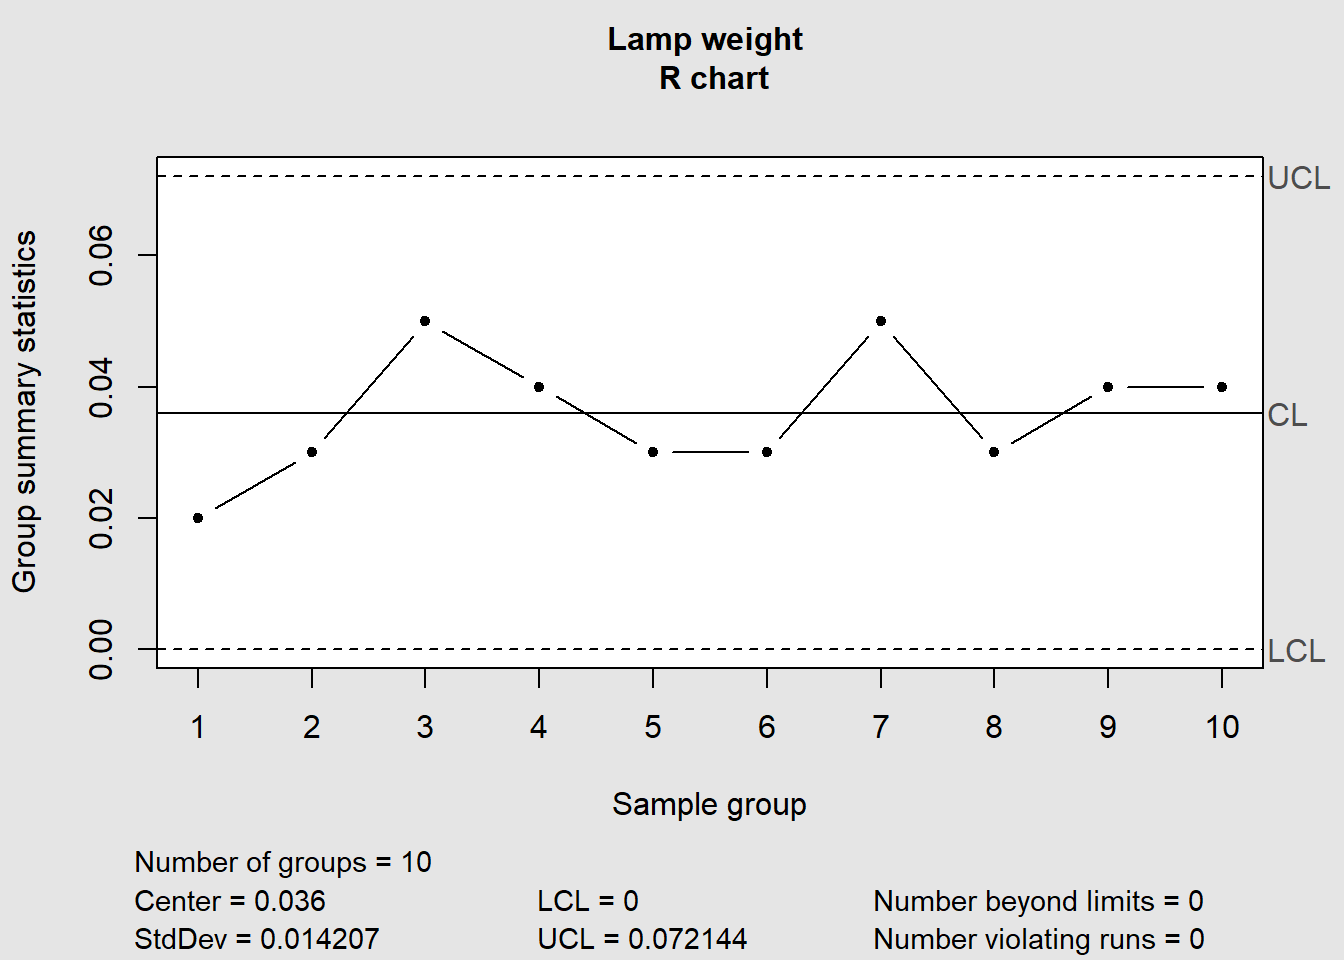
\includegraphics[width=0.8\linewidth]{doe_advanced_files/figure-latex/unnamed-chunk-12-1}

\begin{Shaded}
\begin{Highlighting}[]
\CommentTok{\# And also a scatterplot}
\FunctionTok{ggplot}\NormalTok{(battery\_lm\_factor, }\FunctionTok{aes}\NormalTok{(}\AttributeTok{x =}\NormalTok{ temperature, }\AttributeTok{y =}\NormalTok{ life, }\AttributeTok{color =}\NormalTok{ material)) }\SpecialCharTok{+}
  \FunctionTok{geom\_point}\NormalTok{() }\SpecialCharTok{+}
  \FunctionTok{geom\_smooth}\NormalTok{(}\AttributeTok{method =} \StringTok{"lm"}\NormalTok{, }\AttributeTok{se =} \ConstantTok{FALSE}\NormalTok{) }\CommentTok{\# not clear why the lm line is not plotted, to be investigated}
\end{Highlighting}
\end{Shaded}

\includegraphics[width=0.8\linewidth]{doe_advanced_files/figure-latex/unnamed-chunk-13-1}

\begin{Shaded}
\begin{Highlighting}[]
\CommentTok{\# Just for my curiosity a boxplot for comparison}
\FunctionTok{ggplot}\NormalTok{(battery\_narrow\_factor, }\FunctionTok{aes}\NormalTok{(}\AttributeTok{x =}\NormalTok{ temperature, }\AttributeTok{y =}\NormalTok{ life, }\AttributeTok{color =}\NormalTok{ material)) }\SpecialCharTok{+}
  \FunctionTok{geom\_boxplot}\NormalTok{()}
\end{Highlighting}
\end{Shaded}

\includegraphics[width=0.8\linewidth]{doe_advanced_files/figure-latex/unnamed-chunk-14-1}

\hypertarget{effects-significance}{%
\subsection{Effects significance}\label{effects-significance}}

\begin{Shaded}
\begin{Highlighting}[]
\NormalTok{battery\_aov }\OtherTok{\textless{}{-}} \FunctionTok{aov}\NormalTok{(battery\_lm\_factor)}

\FunctionTok{summary}\NormalTok{(battery\_aov)}
\end{Highlighting}
\end{Shaded}

\begin{verbatim}
                     Df Sum Sq Mean Sq F value   Pr(>F)    
temperature           2  39119   19559  28.968 1.91e-07 ***
material              2  10684    5342   7.911  0.00198 ** 
temperature:material  4   9614    2403   3.560  0.01861 *  
Residuals            27  18231     675                     
---
Signif. codes:  0 '***' 0.001 '**' 0.01 '*' 0.05 '.' 0.1 ' ' 1
\end{verbatim}

\hypertarget{sample-size-calculation}{%
\subsection{Sample size calculation}\label{sample-size-calculation}}

Refer to ``Statistiques faciles avec R,'' page 233.
Cohen's effect size is calculated with the eta squared from the model (intriguing is the same value as the R²\ldots).
In this case with 2 replicates we obtain a power of 90\% and an alpha of 1\%.
I've not managed here to replicate the values from the Montgomery book.

\begin{Shaded}
\begin{Highlighting}[]
\FunctionTok{library}\NormalTok{(pwr)}
\end{Highlighting}
\end{Shaded}

\begin{Shaded}
\begin{Highlighting}[]
\NormalTok{battery\_cohend\_aov }\OtherTok{\textless{}{-}} \DecValTok{40} \SpecialCharTok{/} \DecValTok{25} \CommentTok{\# Cohen\textquotesingle{}s effect size = difference of means / sd}

\FunctionTok{pwr.anova.test}\NormalTok{(}\AttributeTok{k =} \DecValTok{3}\NormalTok{,}
               \AttributeTok{n =} \DecValTok{4}\NormalTok{,}
               \AttributeTok{f =}\NormalTok{ battery\_cohend\_aov,}
               \AttributeTok{sig.level =} \FloatTok{0.05}\NormalTok{)}
\end{Highlighting}
\end{Shaded}

\begin{verbatim}
     Balanced one-way analysis of variance power calculation 

              k = 3
              n = 4
              f = 1.6
      sig.level = 0.05
          power = 0.9892439

NOTE: n is number in each group
\end{verbatim}

I've managed to almost reproduce the book result (I obtained a power of 98\%, in the book 94\%) by calculating the effect size by dividing the life difference of 40 hours by the standard deviation of 25h given in the example and feeding all this in the pwr.anova.test with n = 4 repetitions.

The books ``Statistiques faciles avec R'' proposes to use the eta but this gives very different results.
battery\_eta2 \textless- etaSquared(battery\_aov){[}1{]}
battery\_cohend\_aov \textless- sqrt(battery\_eta2 / (1 - battery\_eta2))

\hypertarget{removing-interaction}{%
\subsection{Removing interaction}\label{removing-interaction}}

\begin{Shaded}
\begin{Highlighting}[]
\CommentTok{\# Removing the interaction from the model:}
\NormalTok{battery\_lm\_factor\_no\_int }\OtherTok{\textless{}{-}} \FunctionTok{lm}\NormalTok{(life }\SpecialCharTok{\textasciitilde{}}\NormalTok{ temperature }\SpecialCharTok{+}\NormalTok{ material,}
                        \AttributeTok{data =}\NormalTok{ battery\_narrow\_factor)}
\NormalTok{battery\_aov\_no\_int }\OtherTok{\textless{}{-}} \FunctionTok{aov}\NormalTok{(battery\_lm\_factor\_no\_int)}

\CommentTok{\# Comparing Anova results with and without:}
\FunctionTok{summary}\NormalTok{(battery\_aov)}
\end{Highlighting}
\end{Shaded}

\begin{verbatim}
                     Df Sum Sq Mean Sq F value   Pr(>F)    
temperature           2  39119   19559  28.968 1.91e-07 ***
material              2  10684    5342   7.911  0.00198 ** 
temperature:material  4   9614    2403   3.560  0.01861 *  
Residuals            27  18231     675                     
---
Signif. codes:  0 '***' 0.001 '**' 0.01 '*' 0.05 '.' 0.1 ' ' 1
\end{verbatim}

\begin{Shaded}
\begin{Highlighting}[]
\FunctionTok{summary}\NormalTok{(battery\_aov\_no\_int)}
\end{Highlighting}
\end{Shaded}

\begin{verbatim}
            Df Sum Sq Mean Sq F value   Pr(>F)    
temperature  2  39119   19559  21.776 1.24e-06 ***
material     2  10684    5342   5.947  0.00651 ** 
Residuals   31  27845     898                     
---
Signif. codes:  0 '***' 0.001 '**' 0.01 '*' 0.05 '.' 0.1 ' ' 1
\end{verbatim}

As noted previously, both main effects are significant (p \textless{} 0.05).

However, as soon as a residual analysis is performed for these data, it becomes clear that the no-interaction model is inadequate:

\begin{Shaded}
\begin{Highlighting}[]
\CommentTok{\# Normality of residuals is worse}
\NormalTok{battery\_residuals\_no\_int }\OtherTok{\textless{}{-}}\NormalTok{ battery\_aov\_no\_int[[}\StringTok{"residuals"}\NormalTok{]]}
\FunctionTok{qqnorm}\NormalTok{(battery\_residuals\_no\_int, }\AttributeTok{datax =} \ConstantTok{TRUE}\NormalTok{);}\FunctionTok{qqline}\NormalTok{(battery\_residuals\_no\_int, }\AttributeTok{datax =} \ConstantTok{TRUE}\NormalTok{)}
\end{Highlighting}
\end{Shaded}

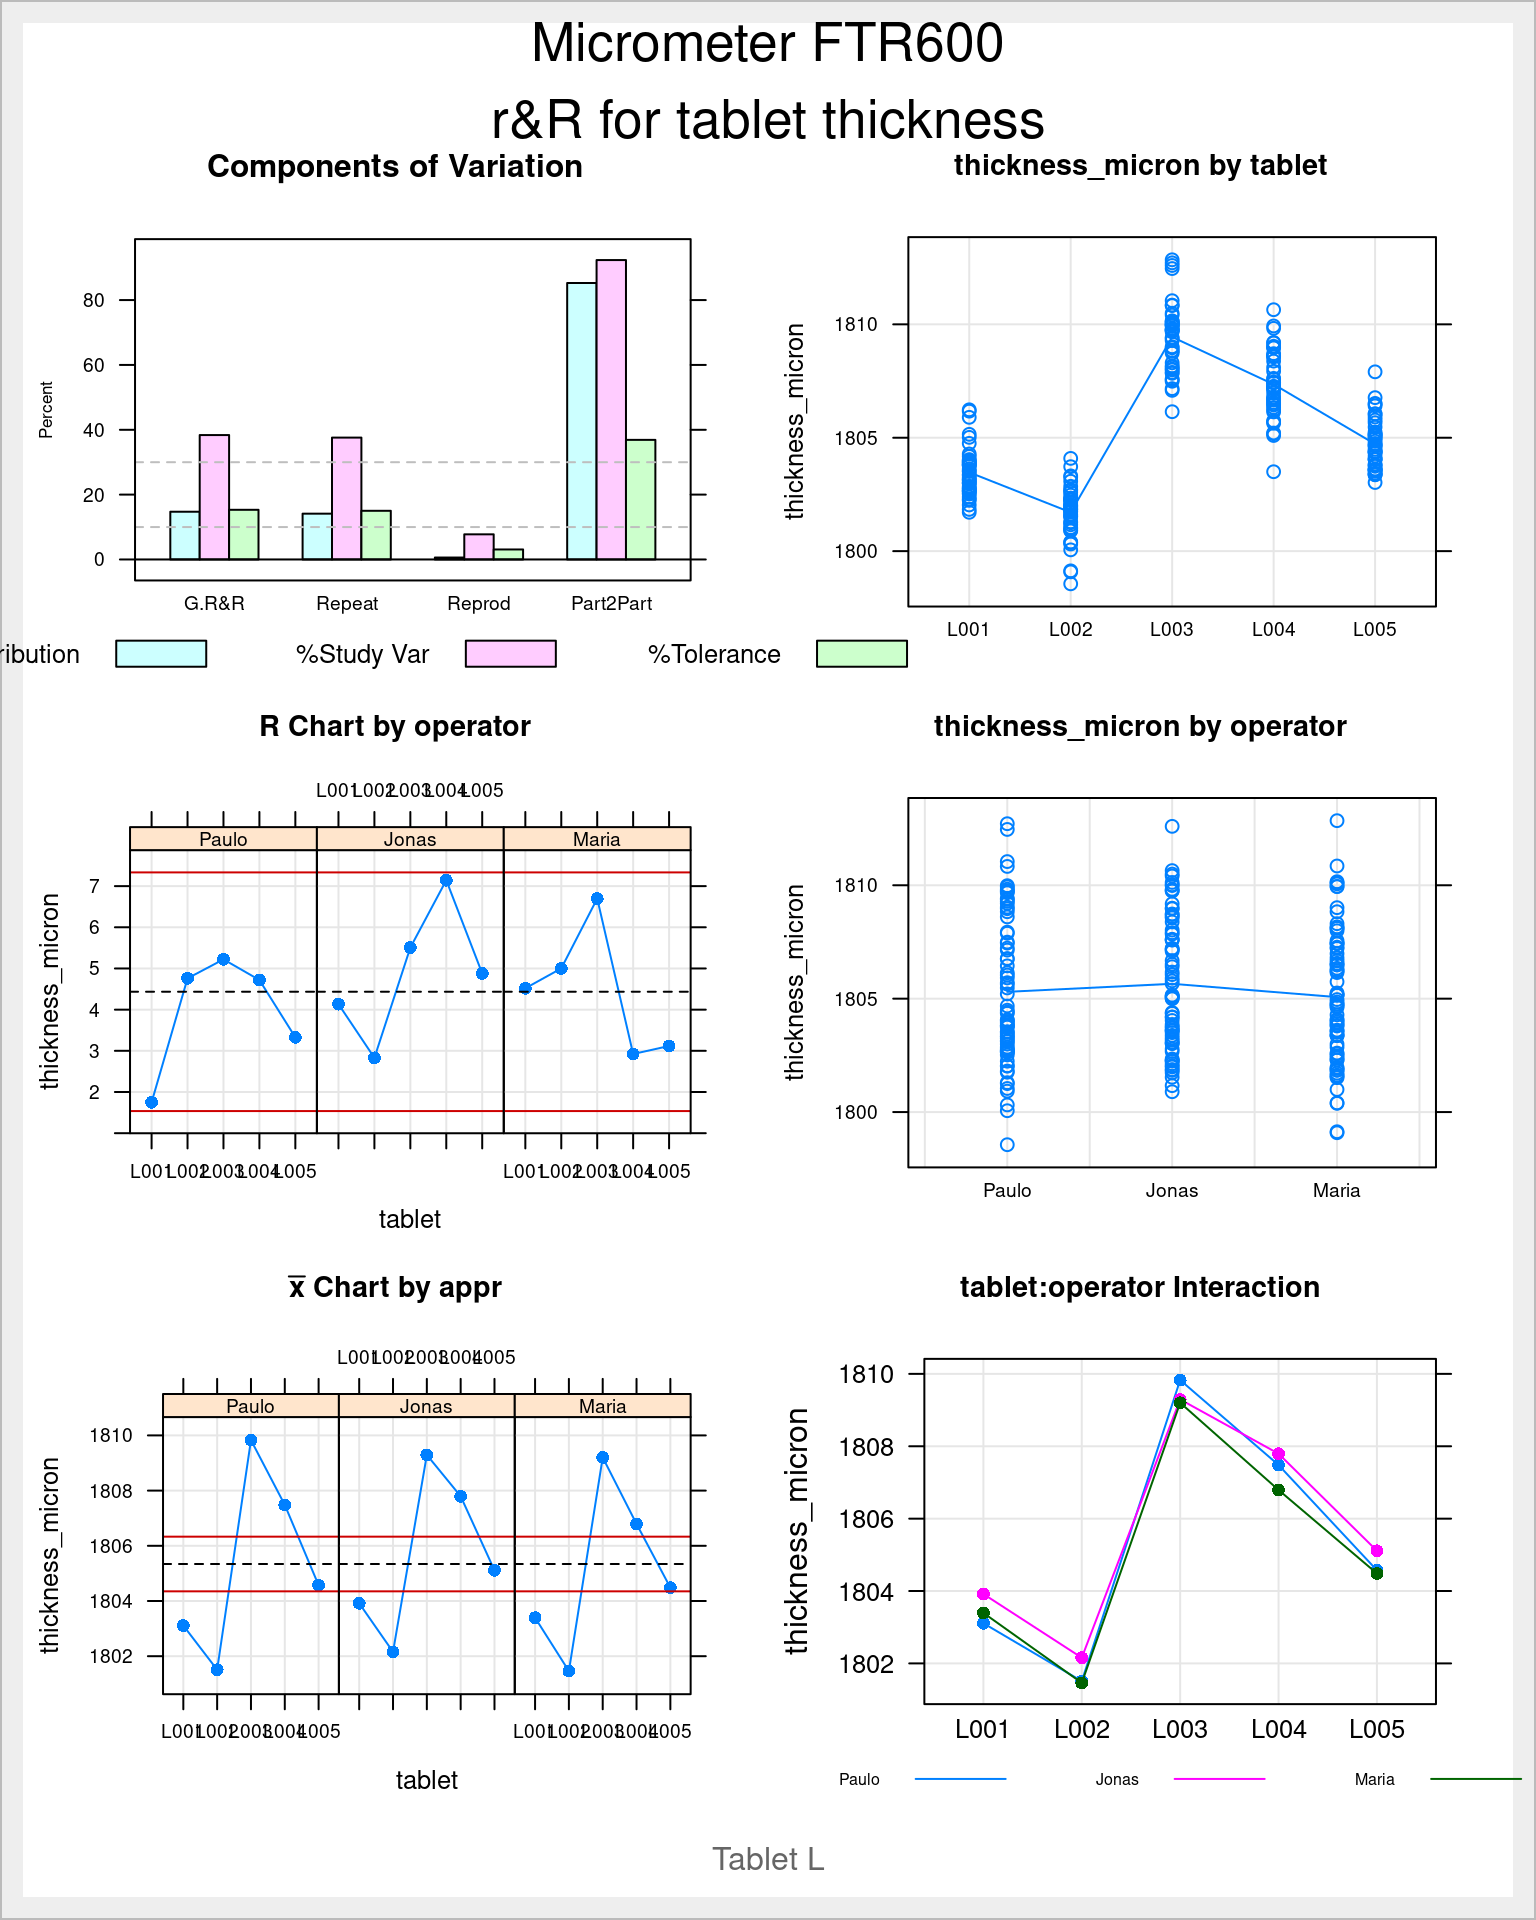
\includegraphics[width=0.8\linewidth]{doe_advanced_files/figure-latex/unnamed-chunk-19-1}

\begin{Shaded}
\begin{Highlighting}[]
\CommentTok{\# But it still passes the Shapiro test}
\FunctionTok{shapiro.test}\NormalTok{(battery\_residuals\_no\_int)}
\end{Highlighting}
\end{Shaded}

\begin{verbatim}
	Shapiro-Wilk normality test

data:  battery_residuals_no_int
W = 0.97846, p-value = 0.6932
\end{verbatim}

\begin{Shaded}
\begin{Highlighting}[]
\CommentTok{\# No standardize residual above 2 either:}
\NormalTok{battery\_tidyfit\_no\_int }\OtherTok{\textless{}{-}} \FunctionTok{augment}\NormalTok{(battery\_lm\_factor\_no\_int)}
\end{Highlighting}
\end{Shaded}

\begin{Shaded}
\begin{Highlighting}[]
\FunctionTok{plot}\NormalTok{(battery\_aov\_no\_int, }\AttributeTok{which =} \DecValTok{2}\NormalTok{)}
\end{Highlighting}
\end{Shaded}

\includegraphics[width=0.8\linewidth]{doe_advanced_files/figure-latex/unnamed-chunk-20-1}

\begin{Shaded}
\begin{Highlighting}[]
\CommentTok{\# It is finally in the plot residuals vs fit that we can clearly see an issue:}
\FunctionTok{plot}\NormalTok{(battery\_aov, }\AttributeTok{which =} \DecValTok{1}\NormalTok{)}
\end{Highlighting}
\end{Shaded}

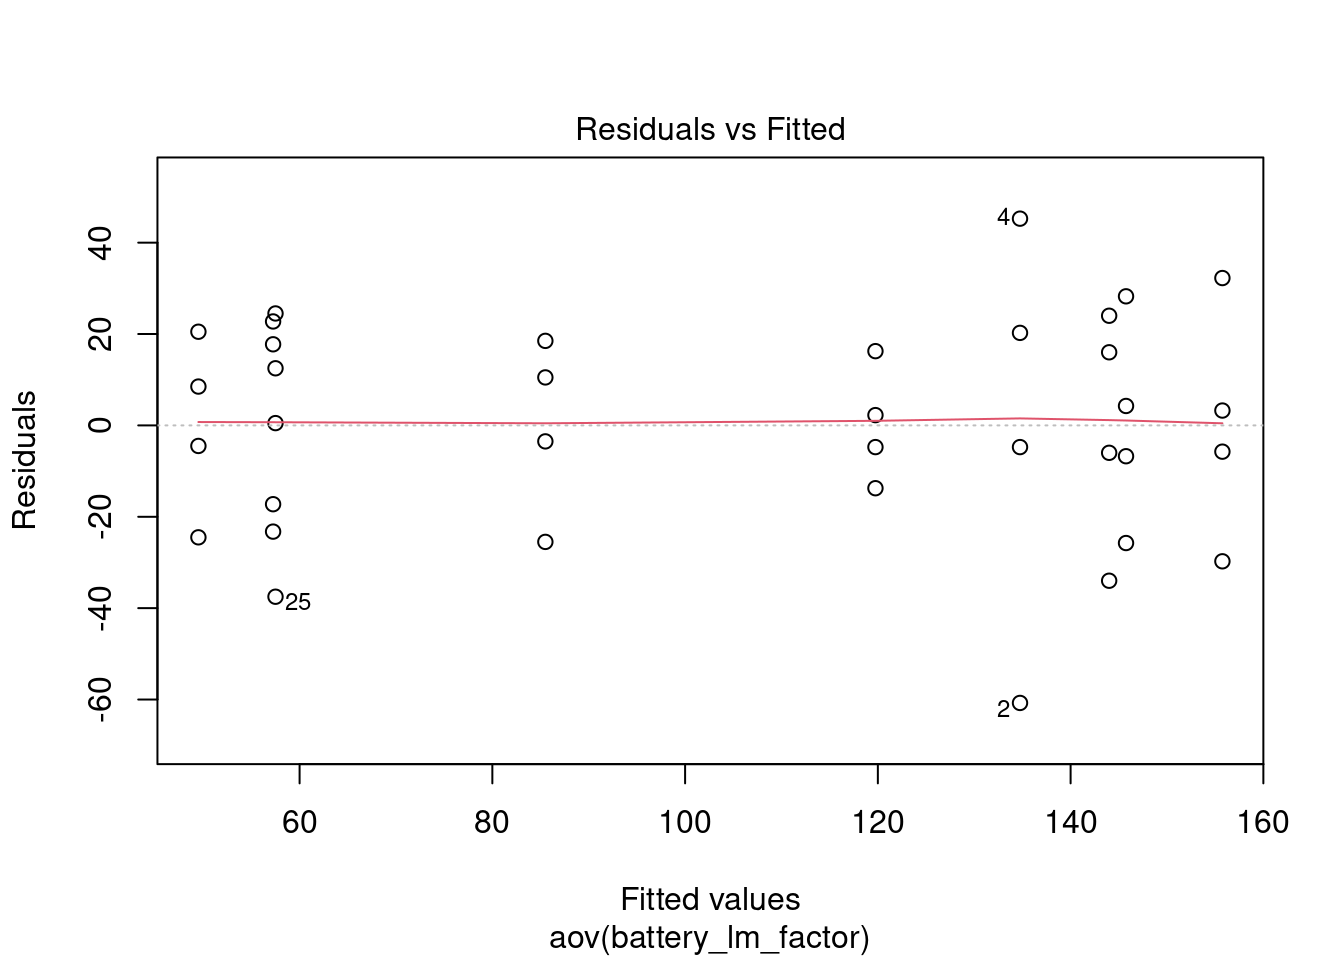
\includegraphics[width=0.8\linewidth]{doe_advanced_files/figure-latex/unnamed-chunk-20-2}

\begin{Shaded}
\begin{Highlighting}[]
\FunctionTok{plot}\NormalTok{(battery\_aov\_no\_int, }\AttributeTok{which =} \DecValTok{1}\NormalTok{)}
\end{Highlighting}
\end{Shaded}

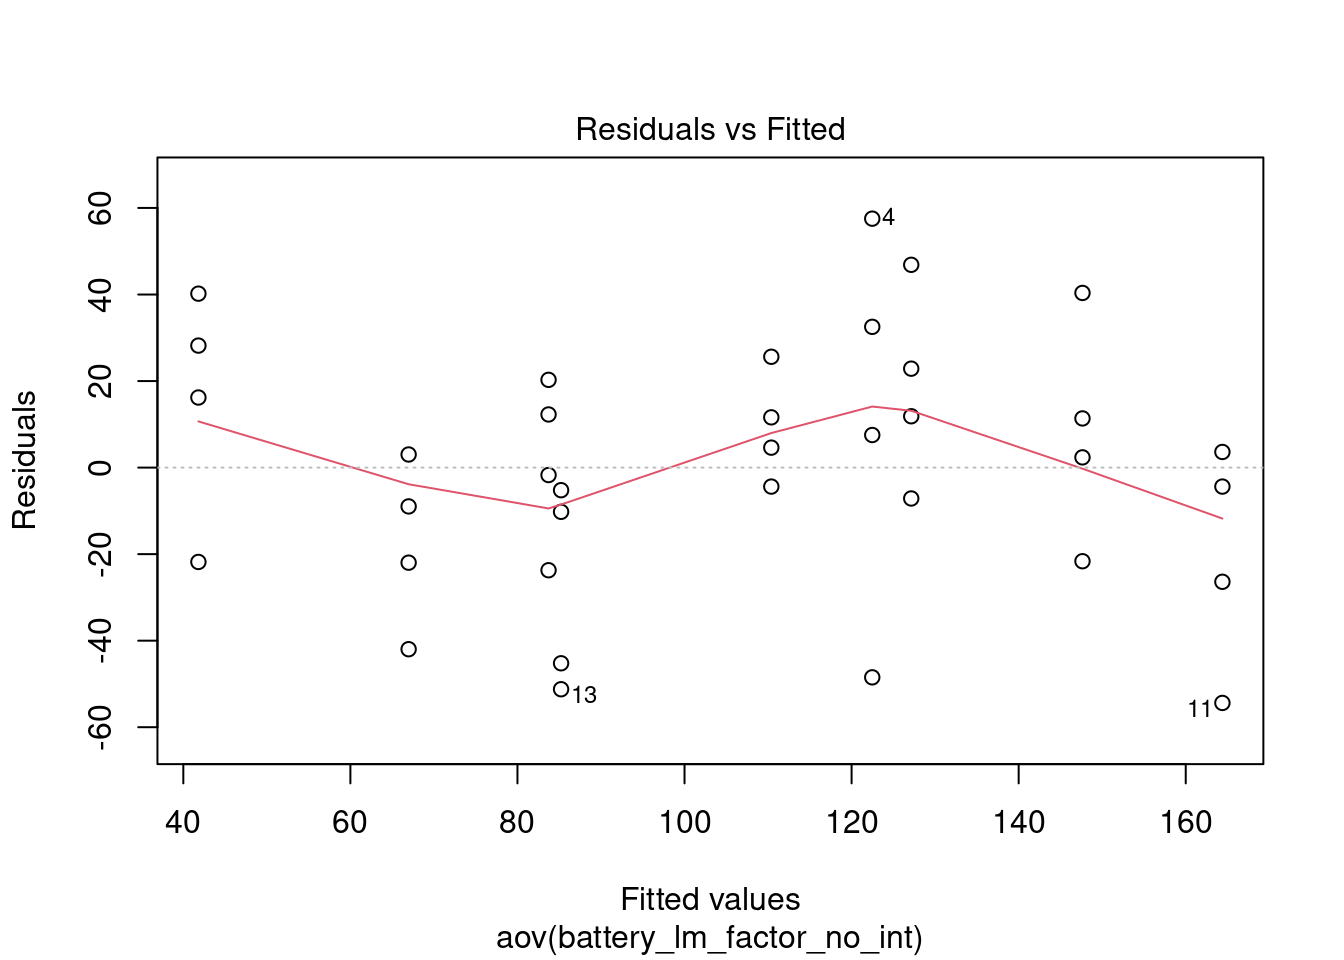
\includegraphics[width=0.8\linewidth]{doe_advanced_files/figure-latex/unnamed-chunk-20-3}

Any pattern in these quantities is suggestive of the presence of interaction. Figure 5.15 shows a distinct pattern as the quantities move from positive to negative to positive to negative again.

\hypertarget{multiple-factors}{%
\section{Multiple factors}\label{multiple-factors}}

Like in the two-factors we must have at least two replicates (n\textgreater2) to determine the sum of squares due to error if all possible interactions are to be included in the model.

Sources of variation for the Anova table for three-factor fixed effects model:
A, B, C, AB, AC, BC, ABC

Soft Drink bottling example

\begin{Shaded}
\begin{Highlighting}[]
\NormalTok{bottling }\OtherTok{\textless{}{-}} \FunctionTok{read.csv}\NormalTok{(}\AttributeTok{sep =} \StringTok{";"}\NormalTok{, }\AttributeTok{header =} \ConstantTok{TRUE}\NormalTok{, }\StringTok{"../industRial/data{-}raw/5\_bottling.csv"}\NormalTok{)}

\NormalTok{bottling\_factor }\OtherTok{\textless{}{-}}\NormalTok{ bottling}
\NormalTok{bottling\_factor}\SpecialCharTok{$}\NormalTok{speed }\OtherTok{\textless{}{-}} \FunctionTok{as.factor}\NormalTok{(bottling}\SpecialCharTok{$}\NormalTok{speed)}
\NormalTok{bottling\_factor}\SpecialCharTok{$}\NormalTok{pressure }\OtherTok{\textless{}{-}} \FunctionTok{as.factor}\NormalTok{(bottling}\SpecialCharTok{$}\NormalTok{pressure)}
\NormalTok{bottling\_factor}\SpecialCharTok{$}\NormalTok{carbonation }\OtherTok{\textless{}{-}} \FunctionTok{as.factor}\NormalTok{(bottling}\SpecialCharTok{$}\NormalTok{carbonation)}
\end{Highlighting}
\end{Shaded}

\hypertarget{main-effects-plots}{%
\subsection{Main effects plots}\label{main-effects-plots}}

\begin{Shaded}
\begin{Highlighting}[]
\CommentTok{\# Main effects plots:}

\CommentTok{\# Percentage of carbonation}
\FunctionTok{ggplot}\NormalTok{(bottling\_factor, }\FunctionTok{aes}\NormalTok{(}\AttributeTok{x =}\NormalTok{ carbonation, }\AttributeTok{y =}\NormalTok{ fill)) }\SpecialCharTok{+}
  \FunctionTok{geom\_boxplot}\NormalTok{()}
\end{Highlighting}
\end{Shaded}

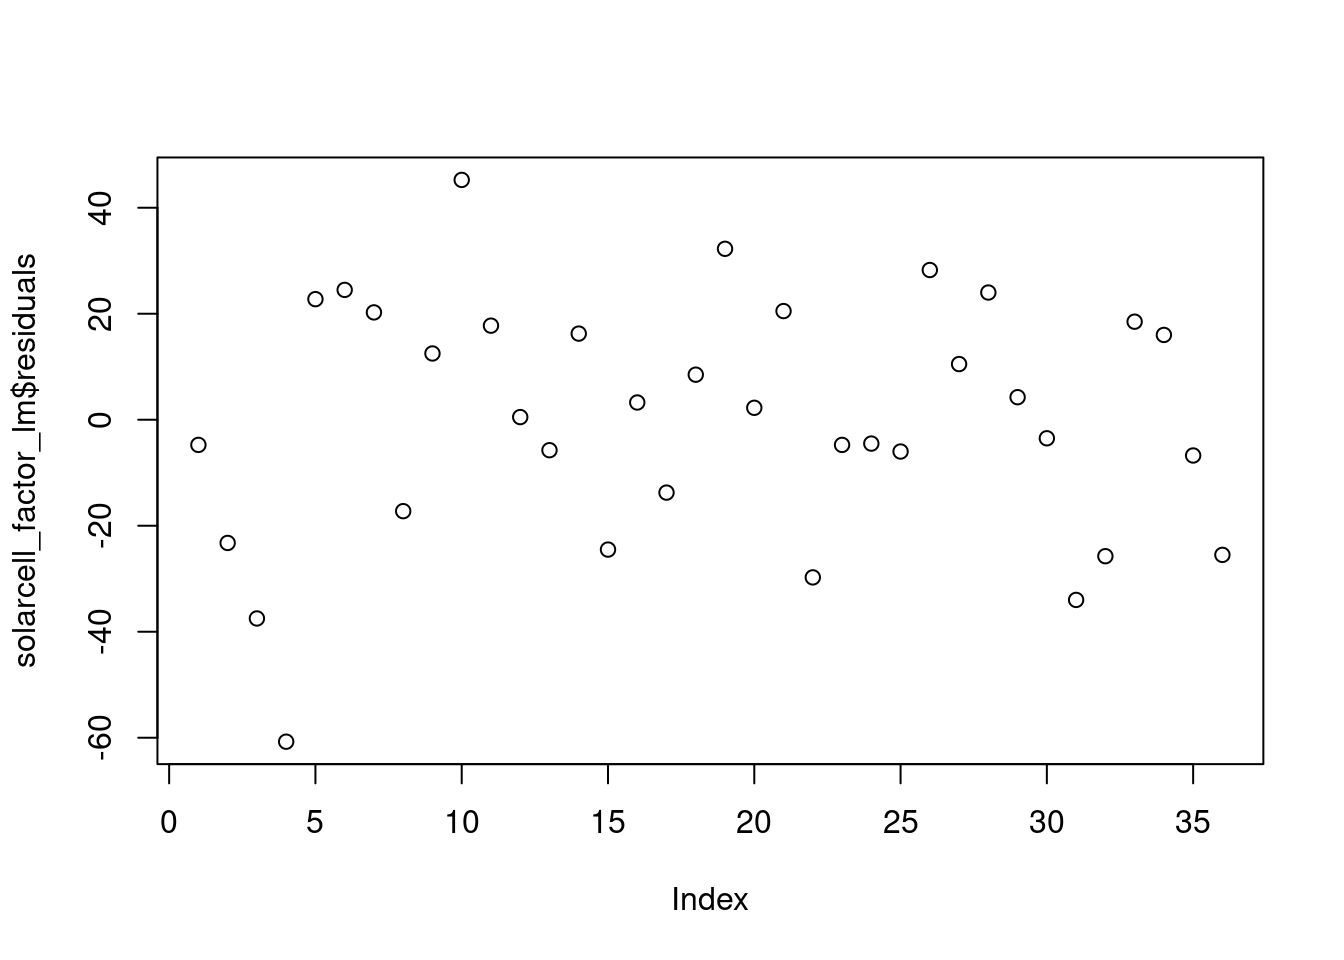
\includegraphics[width=0.8\linewidth]{doe_advanced_files/figure-latex/unnamed-chunk-22-1}

\begin{Shaded}
\begin{Highlighting}[]
\CommentTok{\# Pressure}
\FunctionTok{ggplot}\NormalTok{(bottling\_factor, }\FunctionTok{aes}\NormalTok{(}\AttributeTok{x =}\NormalTok{ pressure, }\AttributeTok{y =}\NormalTok{ fill)) }\SpecialCharTok{+}
  \FunctionTok{geom\_boxplot}\NormalTok{()}
\end{Highlighting}
\end{Shaded}

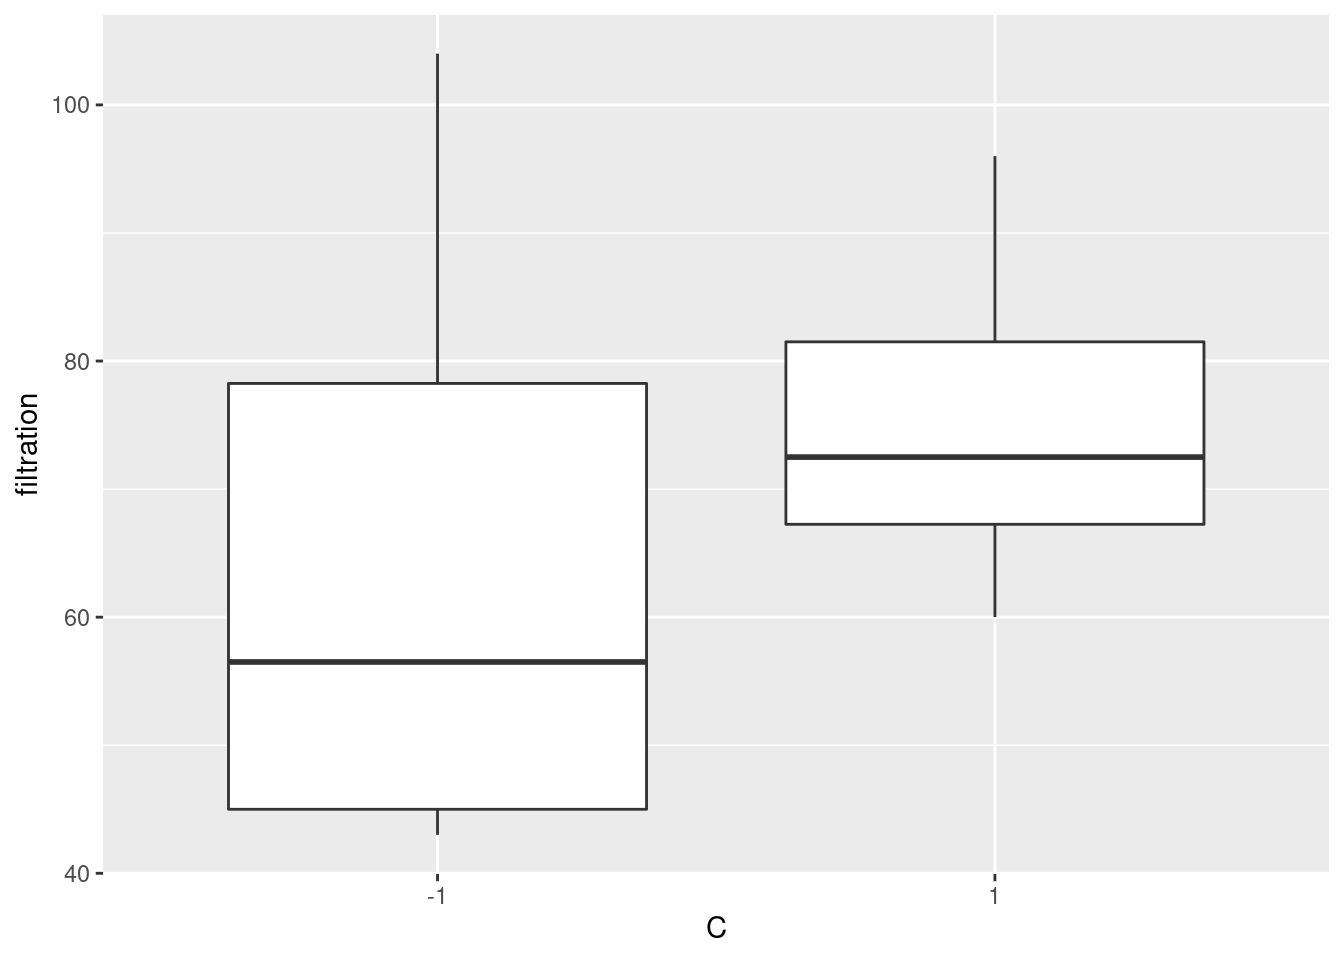
\includegraphics[width=0.8\linewidth]{doe_advanced_files/figure-latex/unnamed-chunk-22-2}

\begin{Shaded}
\begin{Highlighting}[]
\CommentTok{\# Line speed}
\FunctionTok{ggplot}\NormalTok{(bottling\_factor, }\FunctionTok{aes}\NormalTok{(}\AttributeTok{x =}\NormalTok{ speed, }\AttributeTok{y =}\NormalTok{ fill)) }\SpecialCharTok{+}
  \FunctionTok{geom\_boxplot}\NormalTok{()}
\end{Highlighting}
\end{Shaded}

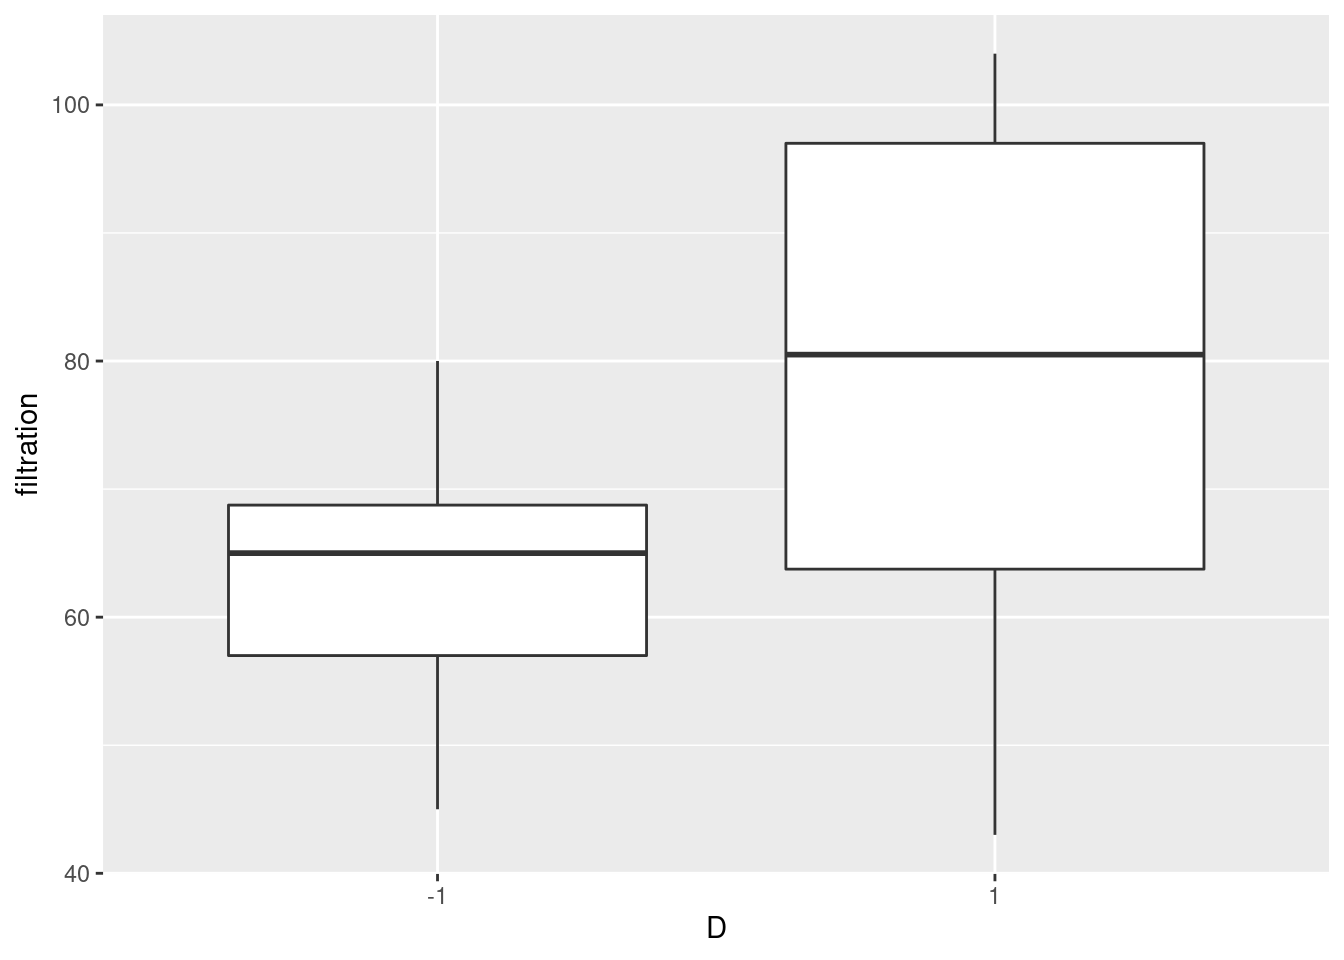
\includegraphics[width=0.8\linewidth]{doe_advanced_files/figure-latex/unnamed-chunk-22-3}

\begin{Shaded}
\begin{Highlighting}[]
\CommentTok{\# Carbonation {-} Pressure interaction}
\CommentTok{\# (corresponds to Montgomery page 210, figure 5.16 d)}
\FunctionTok{ggplot}\NormalTok{(bottling\_factor, }\FunctionTok{aes}\NormalTok{(}\AttributeTok{x =}\NormalTok{ carbonation, }\AttributeTok{y =}\NormalTok{ fill, }\AttributeTok{color =}\NormalTok{ pressure)) }\SpecialCharTok{+}
  \FunctionTok{geom\_boxplot}\NormalTok{()}
\end{Highlighting}
\end{Shaded}

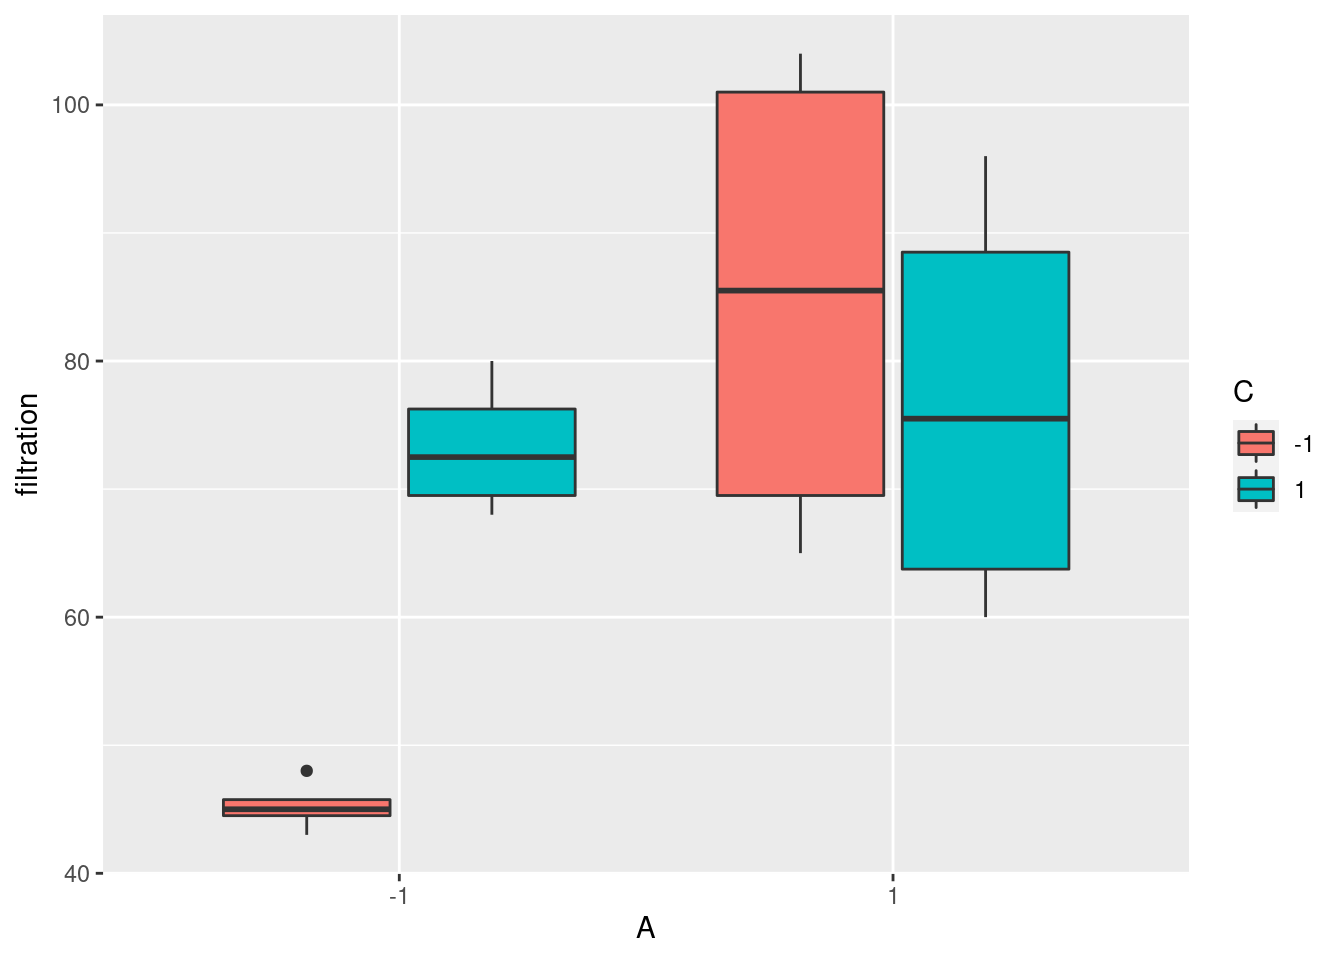
\includegraphics[width=0.8\linewidth]{doe_advanced_files/figure-latex/unnamed-chunk-22-4}

\hypertarget{model-with-3rd-level-interactions}{%
\subsection{Model with 3rd level interactions}\label{model-with-3rd-level-interactions}}

\begin{Shaded}
\begin{Highlighting}[]
\NormalTok{bottling\_lm\_factor }\OtherTok{\textless{}{-}} \FunctionTok{lm}\NormalTok{(fill }\SpecialCharTok{\textasciitilde{}} 
\NormalTok{                           carbonation }\SpecialCharTok{+}\NormalTok{ speed }\SpecialCharTok{+}\NormalTok{ pressure }\SpecialCharTok{+} 
\NormalTok{                           carbonation}\SpecialCharTok{:}\NormalTok{speed }\SpecialCharTok{+} 
\NormalTok{                           carbonation}\SpecialCharTok{:}\NormalTok{pressure }\SpecialCharTok{+} 
\NormalTok{                           speed}\SpecialCharTok{:}\NormalTok{pressure }\SpecialCharTok{+} 
\NormalTok{                           carbonation}\SpecialCharTok{:}\NormalTok{speed}\SpecialCharTok{:}\NormalTok{pressure,}
                           \AttributeTok{data =}\NormalTok{ bottling\_factor}
\NormalTok{  )}
\end{Highlighting}
\end{Shaded}

\hypertarget{model-adequacy-check}{%
\subsection{Model adequacy check}\label{model-adequacy-check}}

\begin{Shaded}
\begin{Highlighting}[]
\NormalTok{bottling\_residuals }\OtherTok{\textless{}{-}}\NormalTok{ bottling\_lm\_factor[[}\StringTok{"residuals"}\NormalTok{]]}
\FunctionTok{qqnorm}\NormalTok{(bottling\_residuals, }\AttributeTok{datax =} \ConstantTok{TRUE}\NormalTok{);}\FunctionTok{qqline}\NormalTok{(bottling\_residuals, }\AttributeTok{datax =} \ConstantTok{TRUE}\NormalTok{)}
\end{Highlighting}
\end{Shaded}

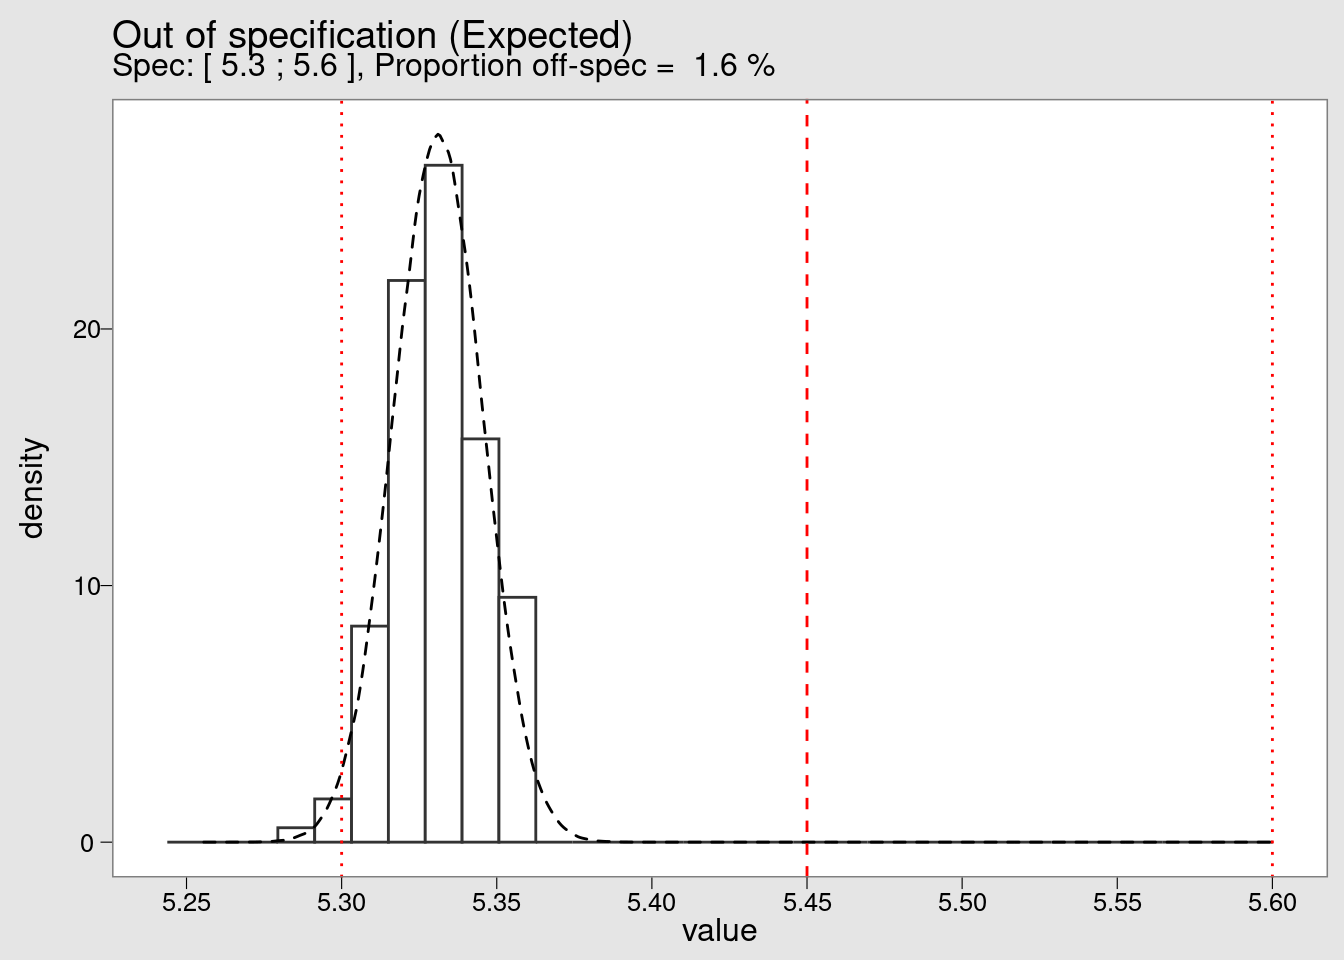
\includegraphics[width=0.8\linewidth]{doe_advanced_files/figure-latex/unnamed-chunk-24-1}

\begin{Shaded}
\begin{Highlighting}[]
\FunctionTok{shapiro.test}\NormalTok{(bottling\_residuals)}
\end{Highlighting}
\end{Shaded}

\begin{verbatim}
	Shapiro-Wilk normality test

data:  bottling_residuals
W = 0.86322, p-value = 0.003885
\end{verbatim}

\begin{Shaded}
\begin{Highlighting}[]
\NormalTok{bottling\_tidyfit }\OtherTok{\textless{}{-}} \FunctionTok{augment}\NormalTok{(bottling\_lm\_factor)}
\end{Highlighting}
\end{Shaded}

\begin{Shaded}
\begin{Highlighting}[]
\FunctionTok{plot}\NormalTok{(bottling\_lm\_factor, }\AttributeTok{which =} \DecValTok{2}\NormalTok{)}
\end{Highlighting}
\end{Shaded}

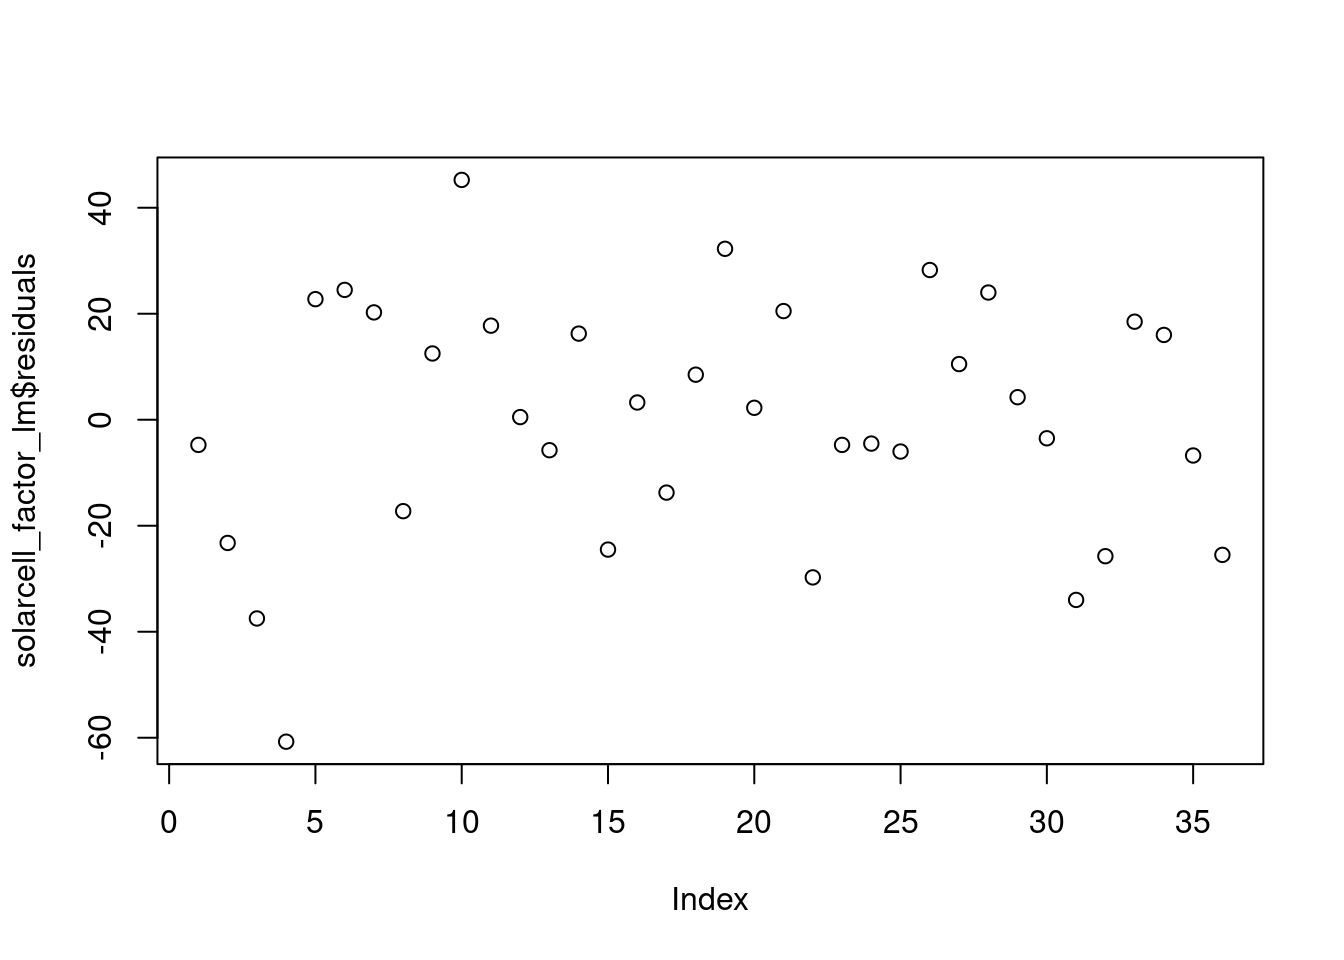
\includegraphics[width=0.8\linewidth]{doe_advanced_files/figure-latex/unnamed-chunk-25-1}

\begin{Shaded}
\begin{Highlighting}[]
\CommentTok{\# It is finally in the plot residuals vs fit that we can clearly see an issue:}
\FunctionTok{plot}\NormalTok{(bottling\_lm\_factor, }\AttributeTok{which =} \DecValTok{1}\NormalTok{)}
\end{Highlighting}
\end{Shaded}

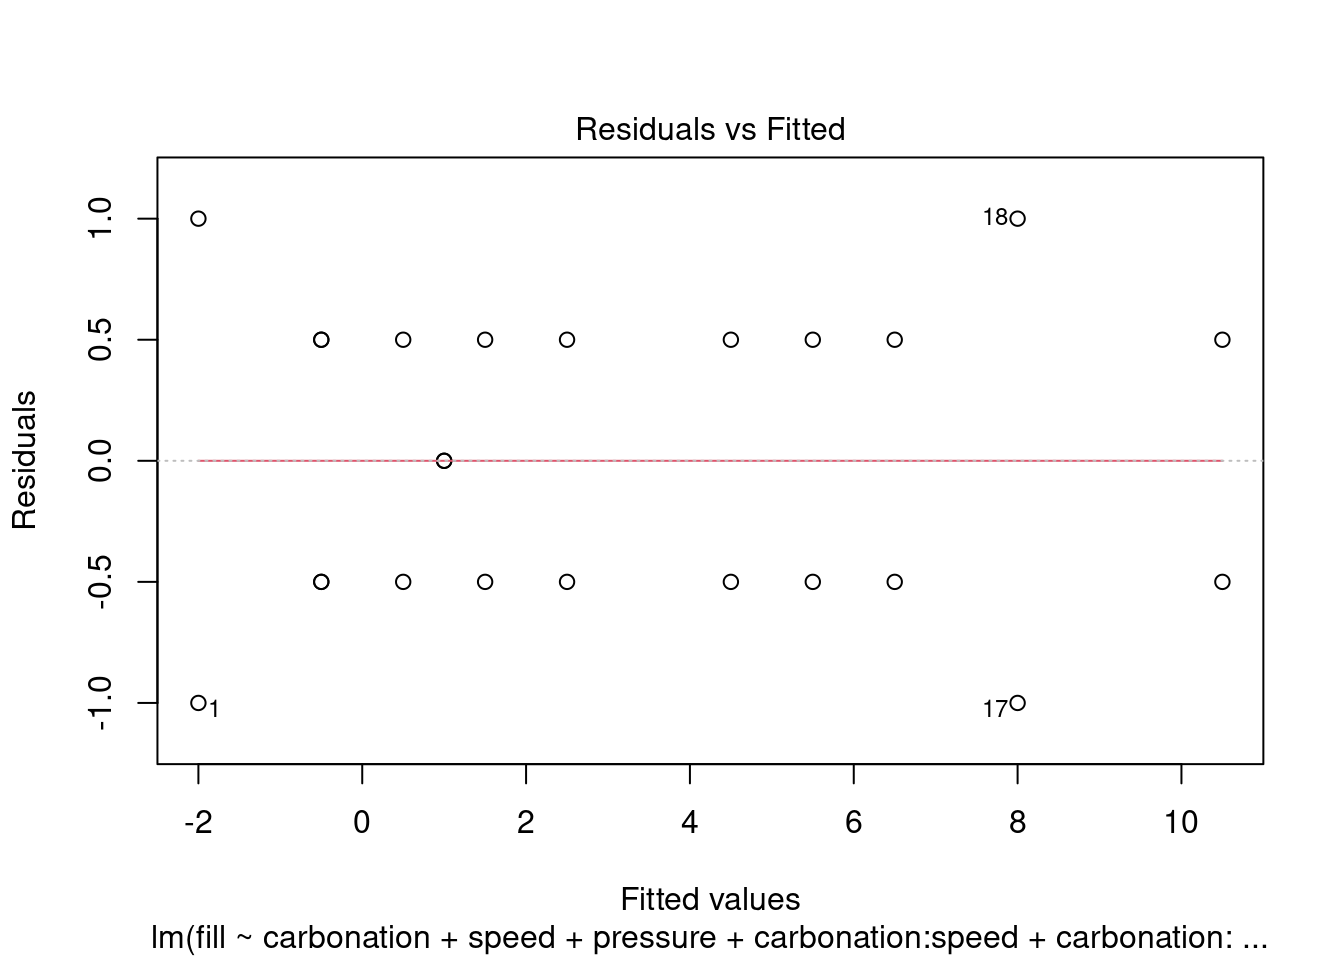
\includegraphics[width=0.8\linewidth]{doe_advanced_files/figure-latex/unnamed-chunk-25-2}

\hypertarget{anova-with-3rd-level-interactions}{%
\subsection{Anova with 3rd level interactions}\label{anova-with-3rd-level-interactions}}

\begin{Shaded}
\begin{Highlighting}[]
\NormalTok{bottling\_aov }\OtherTok{\textless{}{-}} \FunctionTok{aov}\NormalTok{(bottling\_lm\_factor)}
\FunctionTok{summary}\NormalTok{(bottling\_aov)}
\end{Highlighting}
\end{Shaded}

\begin{verbatim}
                           Df Sum Sq Mean Sq F value   Pr(>F)    
carbonation                 2 252.75  126.38 178.412 1.19e-09 ***
speed                       1  22.04   22.04  31.118  0.00012 ***
pressure                    1  45.38   45.38  64.059 3.74e-06 ***
carbonation:speed           2   0.58    0.29   0.412  0.67149    
carbonation:pressure        2   5.25    2.62   3.706  0.05581 .  
speed:pressure              1   1.04    1.04   1.471  0.24859    
carbonation:speed:pressure  2   1.08    0.54   0.765  0.48687    
Residuals                  12   8.50    0.71                     
---
Signif. codes:  0 '***' 0.001 '**' 0.01 '*' 0.05 '.' 0.1 ' ' 1
\end{verbatim}

We see that the percentage of carbonation, operating pressure, and line speed significantly affect the fill volume (p \textless{} 0.05)
The carbonation-pressure interaction F ratio has a P-value of 0.0558, indicating
some interaction between these factors.

\hypertarget{factorial-design}{%
\section{2\^{}2 factorial design}\label{factorial-design}}

Extremely important class of designs, specially in factor screening experiments.
In this case factors only have 2 levels. Assumptions:
(1) the factors are fixed
(2) the designs are completely randomized
(3) the usual normality assumptions are satisfied
the response is approximately linear over the range of the factor levels chose

The 2k design is particularly useful in the early stages of experimental work when many
factors are likely to be investigated. It provides the smallest number of runs with which k factors
can be studied in a complete factorial design. Consequently, these designs are widely
used in factor screening experiments.

The Chemical Process example

\begin{Shaded}
\begin{Highlighting}[]
\NormalTok{chm }\OtherTok{\textless{}{-}} \FunctionTok{read.csv}\NormalTok{(}\AttributeTok{sep =} \StringTok{";"}\NormalTok{, }\AttributeTok{header =} \ConstantTok{TRUE}\NormalTok{, }\StringTok{"../industRial/data{-}raw/6\_chemical.csv"}\NormalTok{)}

\CommentTok{\# Converting into a narrow table with a factor for utilisation with ggplot2}
\CommentTok{\# syntax: gather(data, }
\CommentTok{\#               name of the new key column (where the columns names go to), }
\CommentTok{\#               name of the new value column (where the values go), }
\CommentTok{\#               name of the columns to be gathered)}
\NormalTok{chmn }\OtherTok{\textless{}{-}}\NormalTok{ chm }\SpecialCharTok{\%\textgreater{}\%} \CommentTok{\# "chm narrow dataframe"}
  \FunctionTok{gather}\NormalTok{(replicate, yield, I, II, III)}
\end{Highlighting}
\end{Shaded}

\hypertarget{linear-model-with-and--}{%
\subsection{Linear model with + and -}\label{linear-model-with-and--}}

\begin{Shaded}
\begin{Highlighting}[]
\NormalTok{chmn\_lm }\OtherTok{\textless{}{-}} \FunctionTok{lm}\NormalTok{(yield }\SpecialCharTok{\textasciitilde{}}\NormalTok{ A }\SpecialCharTok{+}\NormalTok{ B }\SpecialCharTok{+}\NormalTok{ A}\SpecialCharTok{:}\NormalTok{B, }\AttributeTok{data =}\NormalTok{ chmn)}
\end{Highlighting}
\end{Shaded}

\begin{Shaded}
\begin{Highlighting}[]
\FunctionTok{par}\NormalTok{(}\AttributeTok{mfrow =} \FunctionTok{c}\NormalTok{(}\DecValTok{2}\NormalTok{,}\DecValTok{2}\NormalTok{))}
\FunctionTok{plot}\NormalTok{(chmn\_lm)}
\end{Highlighting}
\end{Shaded}

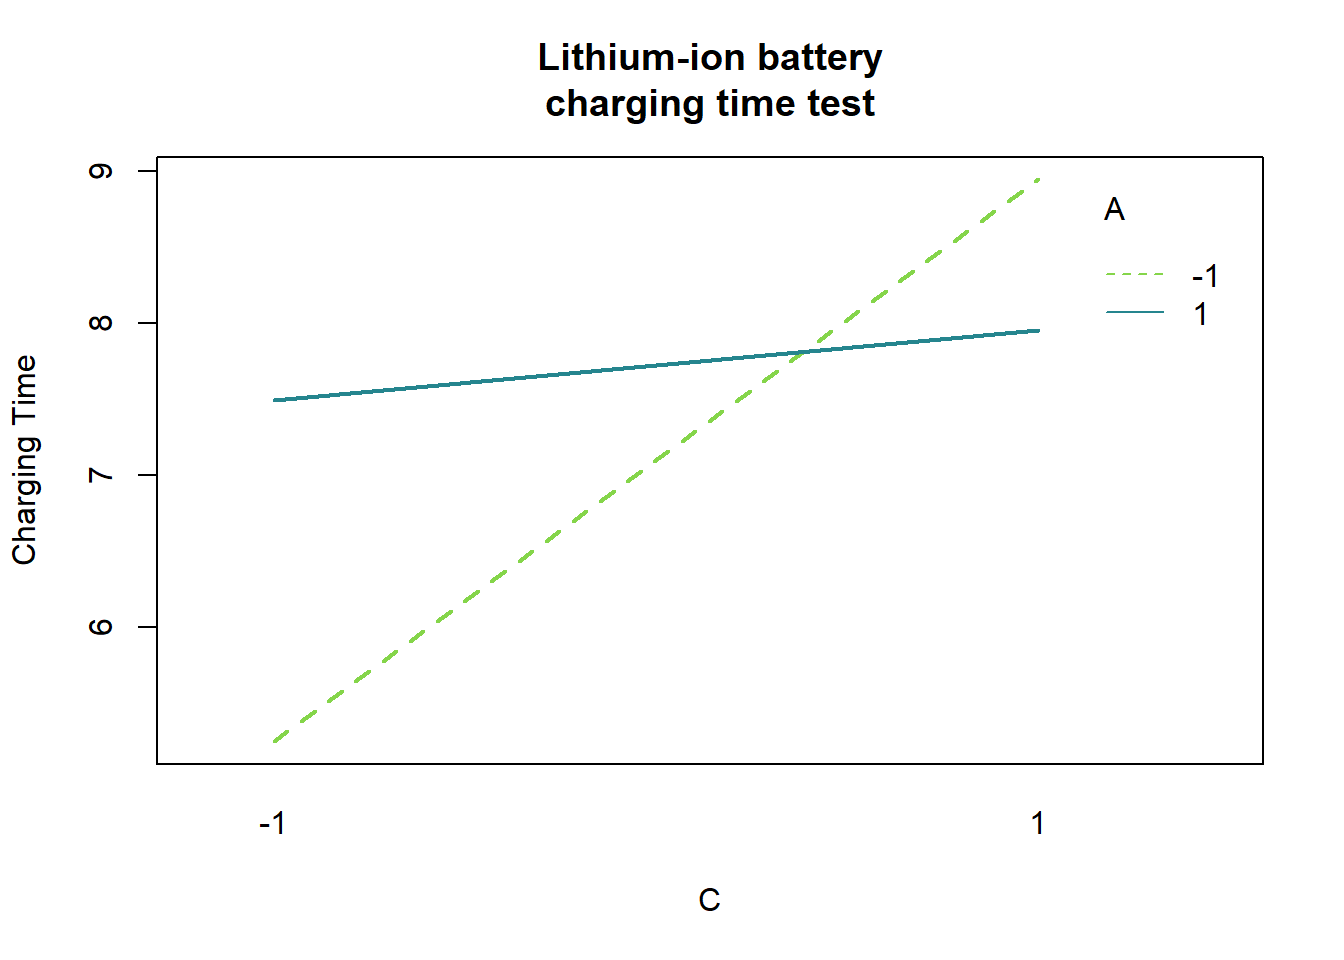
\includegraphics[width=0.8\linewidth]{doe_advanced_files/figure-latex/unnamed-chunk-29-1}

\hypertarget{anova-with-and--}{%
\subsection{Anova with + and -}\label{anova-with-and--}}

\begin{Shaded}
\begin{Highlighting}[]
\NormalTok{chmn\_aov }\OtherTok{\textless{}{-}} \FunctionTok{aov}\NormalTok{(chmn\_lm)}
\FunctionTok{summary}\NormalTok{(chmn\_aov)}
\end{Highlighting}
\end{Shaded}

\begin{verbatim}
            Df Sum Sq Mean Sq F value   Pr(>F)    
A            1 208.33  208.33  53.191 8.44e-05 ***
B            1  75.00   75.00  19.149  0.00236 ** 
A:B          1   8.33    8.33   2.128  0.18278    
Residuals    8  31.33    3.92                     
---
Signif. codes:  0 '***' 0.001 '**' 0.01 '*' 0.05 '.' 0.1 ' ' 1
\end{verbatim}

\hypertarget{interaction-plots-with-sd-bars}{%
\subsection{Interaction plots with sd bars}\label{interaction-plots-with-sd-bars}}

\begin{Shaded}
\begin{Highlighting}[]
\FunctionTok{library}\NormalTok{(RcmdrMisc)}
\end{Highlighting}
\end{Shaded}

\begin{Shaded}
\begin{Highlighting}[]
\CommentTok{\# Alternative plot from the RcmdrMisc package ("Stats facile avec R")}
\FunctionTok{par}\NormalTok{(}\AttributeTok{mfrow =} \FunctionTok{c}\NormalTok{(}\DecValTok{1}\NormalTok{,}\DecValTok{1}\NormalTok{))}
\FunctionTok{plotMeans}\NormalTok{(}\AttributeTok{response =}\NormalTok{ chmn}\SpecialCharTok{$}\NormalTok{yield,}
          \AttributeTok{factor1 =}\NormalTok{ chmn}\SpecialCharTok{$}\NormalTok{A,}
          \AttributeTok{factor2 =}\NormalTok{ chmn}\SpecialCharTok{$}\NormalTok{B)}
\end{Highlighting}
\end{Shaded}

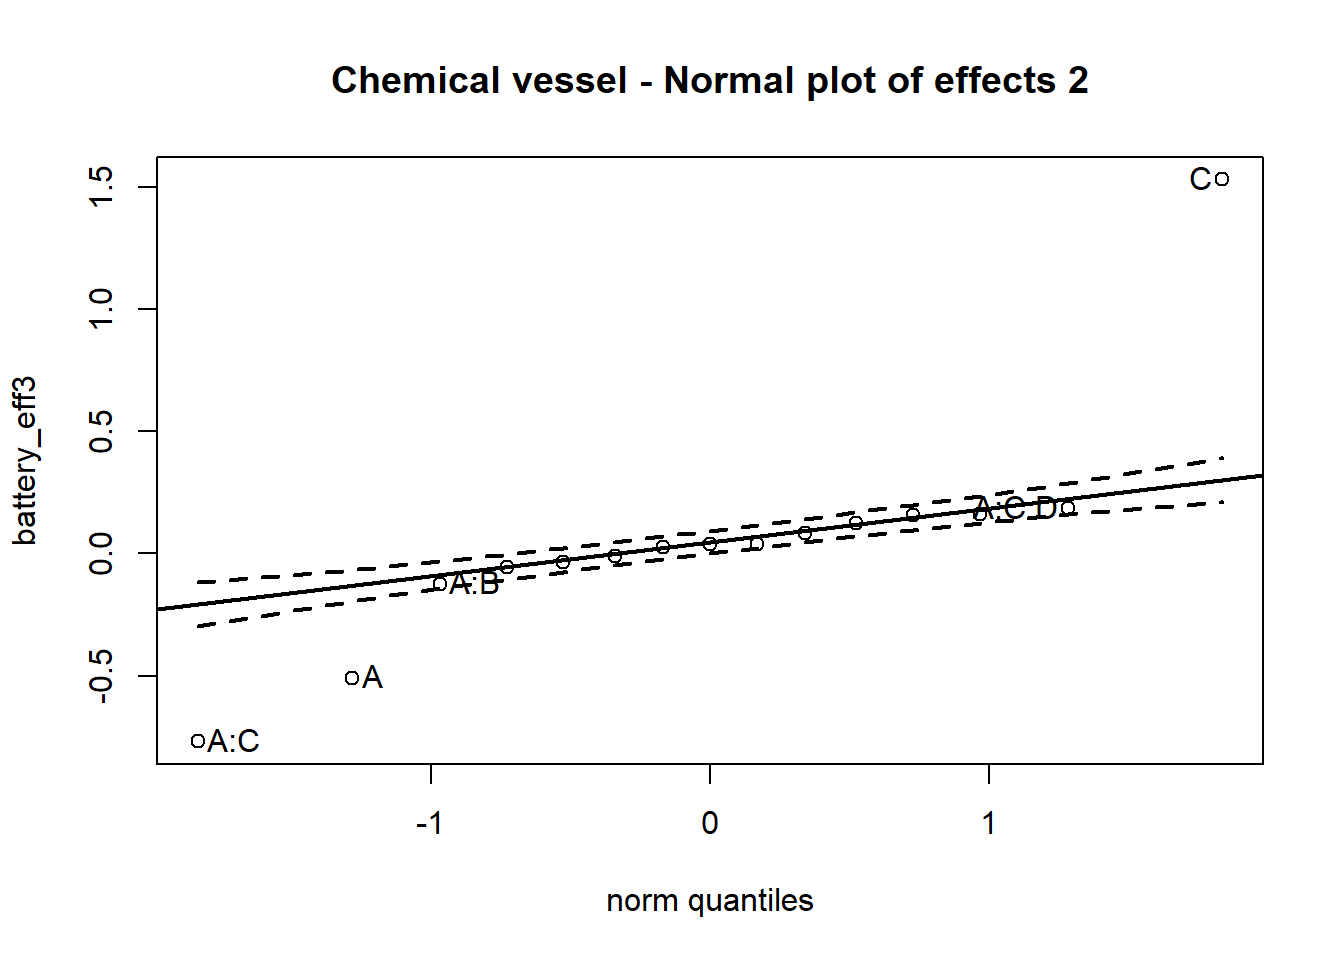
\includegraphics[width=0.8\linewidth]{doe_advanced_files/figure-latex/unnamed-chunk-32-1}

\hypertarget{outputs-correlation}{%
\subsection{Outputs correlation}\label{outputs-correlation}}

\hypertarget{correlation-matrix}{%
\subsubsection{Correlation matrix}\label{correlation-matrix}}

\hypertarget{network-diagrams}{%
\subsubsection{Network diagrams}\label{network-diagrams}}

\hypertarget{levels-coding-with-1-and--1}{%
\subsection{Levels coding with +1 and -1}\label{levels-coding-with-1-and--1}}

Effects
Fit the regression equation, with versions of the factors, coded as numeric!, −1 for low levels, and +1 for high levels.

\begin{Shaded}
\begin{Highlighting}[]
\NormalTok{coded }\OtherTok{\textless{}{-}} \ControlFlowTok{function}\NormalTok{(x) \{}
  \FunctionTok{ifelse}\NormalTok{(x }\SpecialCharTok{==}\NormalTok{ x[}\DecValTok{1}\NormalTok{], }\SpecialCharTok{{-}}\DecValTok{1}\NormalTok{, }\DecValTok{1}\NormalTok{)}
\NormalTok{\}}
\end{Highlighting}
\end{Shaded}

\hypertarget{model-with-1-and--1}{%
\subsection{Model with 1 and -1}\label{model-with-1-and--1}}

\begin{Shaded}
\begin{Highlighting}[]
\NormalTok{chmn2 }\OtherTok{\textless{}{-}} \FunctionTok{within}\NormalTok{(chmn, \{cA }\OtherTok{=} \FunctionTok{coded}\NormalTok{(A); cB }\OtherTok{=} \FunctionTok{coded}\NormalTok{(B)\})}
\NormalTok{chmn2 }\OtherTok{\textless{}{-}} \FunctionTok{select}\NormalTok{(chmn2, A, B, replicate, yield, cA, cB)}
\NormalTok{chmn2\_lm }\OtherTok{\textless{}{-}} \FunctionTok{lm}\NormalTok{(yield }\SpecialCharTok{\textasciitilde{}}\NormalTok{ cA }\SpecialCharTok{*}\NormalTok{ cB, }\AttributeTok{data =}\NormalTok{ chmn2)}
\FunctionTok{summary}\NormalTok{(chmn2\_lm)}
\end{Highlighting}
\end{Shaded}

\begin{verbatim}
Call:
lm(formula = yield ~ cA * cB, data = chmn2)

Residuals:
   Min     1Q Median     3Q    Max 
-2.000 -1.333 -0.500  1.083  3.000 

Coefficients:
            Estimate Std. Error t value Pr(>|t|)    
(Intercept)  27.5000     0.5713  48.135 3.84e-11 ***
cA            4.1667     0.5713   7.293 8.44e-05 ***
cB           -2.5000     0.5713  -4.376  0.00236 ** 
cA:cB         0.8333     0.5713   1.459  0.18278    
---
Signif. codes:  0 '***' 0.001 '**' 0.01 '*' 0.05 '.' 0.1 ' ' 1

Residual standard error: 1.979 on 8 degrees of freedom
Multiple R-squared:  0.903,	Adjusted R-squared:  0.8666 
F-statistic: 24.82 on 3 and 8 DF,  p-value: 0.0002093
\end{verbatim}

\hypertarget{prediction-with-1-and--1}{%
\subsection{Prediction with 1 and -1}\label{prediction-with-1-and--1}}

\begin{Shaded}
\begin{Highlighting}[]
\NormalTok{chmn\_new }\OtherTok{\textless{}{-}} \FunctionTok{data.frame}\NormalTok{(}\AttributeTok{cA =} \DecValTok{1}\NormalTok{, }\AttributeTok{cB =} \DecValTok{1}\NormalTok{)}
\FunctionTok{predict}\NormalTok{(chmn2\_lm, }\AttributeTok{newdata =}\NormalTok{ chmn\_new)}
\end{Highlighting}
\end{Shaded}

\begin{verbatim}
 1 
30 
\end{verbatim}

Compare with predicted table below (the same values are found!)

\begin{Shaded}
\begin{Highlighting}[]
\NormalTok{chmn2\_tidy }\OtherTok{\textless{}{-}} \FunctionTok{augment}\NormalTok{(chmn2\_lm)}
\end{Highlighting}
\end{Shaded}

A coefficient in a regression equation is the change in the response when the corresponding variable changes by +1.

As A or B changes from its low level to its high level, the coded variable changes by 1 − (−1) = +2, so the change in the response is twice the regression coefficient.
So the effects and interaction(s) are twice the values in the ``Estimate'' column.
--\textgreater{} These regression coefficients are often called effects and interactions, even though they differ from the definitions given earlier.

\hypertarget{factorial-design-1}{%
\section{2\^{}3 factorial design}\label{factorial-design-1}}

The plasma etching example

A - gap in cm
B - flow
C - power in W
response - etch rate in Angstrom/m

\begin{Shaded}
\begin{Highlighting}[]
\NormalTok{pls }\OtherTok{\textless{}{-}} \FunctionTok{read.csv}\NormalTok{(}\StringTok{"../industRial/data{-}raw/6{-}3\_plasma.csv"}\NormalTok{)}
\NormalTok{pls}\SpecialCharTok{$}\NormalTok{A }\OtherTok{\textless{}{-}} \FunctionTok{as.factor}\NormalTok{(pls}\SpecialCharTok{$}\NormalTok{A)}
\NormalTok{pls}\SpecialCharTok{$}\NormalTok{B }\OtherTok{\textless{}{-}} \FunctionTok{as.factor}\NormalTok{(pls}\SpecialCharTok{$}\NormalTok{B)}
\NormalTok{pls}\SpecialCharTok{$}\NormalTok{C }\OtherTok{\textless{}{-}} \FunctionTok{as.factor}\NormalTok{(pls}\SpecialCharTok{$}\NormalTok{C)}

\NormalTok{plsn }\OtherTok{\textless{}{-}}\NormalTok{ pls }\SpecialCharTok{\%\textgreater{}\%} \CommentTok{\# "chm narrow dataframe"}
  \FunctionTok{gather}\NormalTok{(replicate, etch, Rep1, Rep2)}
\end{Highlighting}
\end{Shaded}

\hypertarget{main-effects-box-plots}{%
\subsection{Main effects box plots}\label{main-effects-box-plots}}

\begin{Shaded}
\begin{Highlighting}[]
\CommentTok{\# Main effect of A}
\FunctionTok{ggplot}\NormalTok{(plsn, }\FunctionTok{aes}\NormalTok{(}\AttributeTok{x =}\NormalTok{ A, }\AttributeTok{y =}\NormalTok{ etch)) }\SpecialCharTok{+}
  \FunctionTok{geom\_boxplot}\NormalTok{()}
\end{Highlighting}
\end{Shaded}

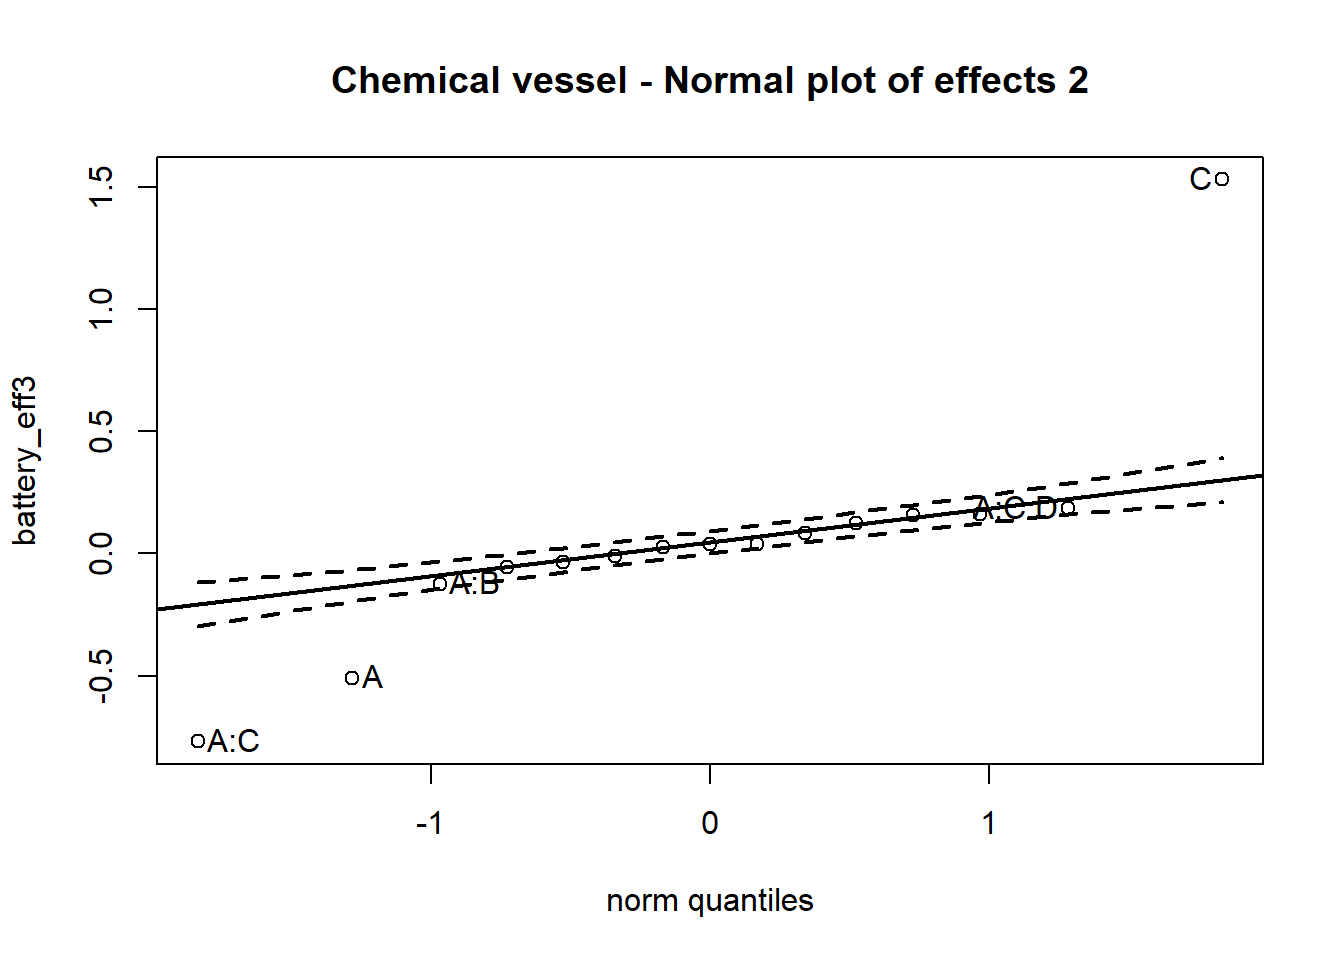
\includegraphics[width=0.8\linewidth]{doe_advanced_files/figure-latex/unnamed-chunk-38-1}

\begin{Shaded}
\begin{Highlighting}[]
\CommentTok{\# Interaction gap {-} power}
\FunctionTok{with}\NormalTok{(plsn, }\FunctionTok{interaction.plot}\NormalTok{(A, C, etch, }\AttributeTok{type =} \StringTok{"b"}\NormalTok{))}
\end{Highlighting}
\end{Shaded}

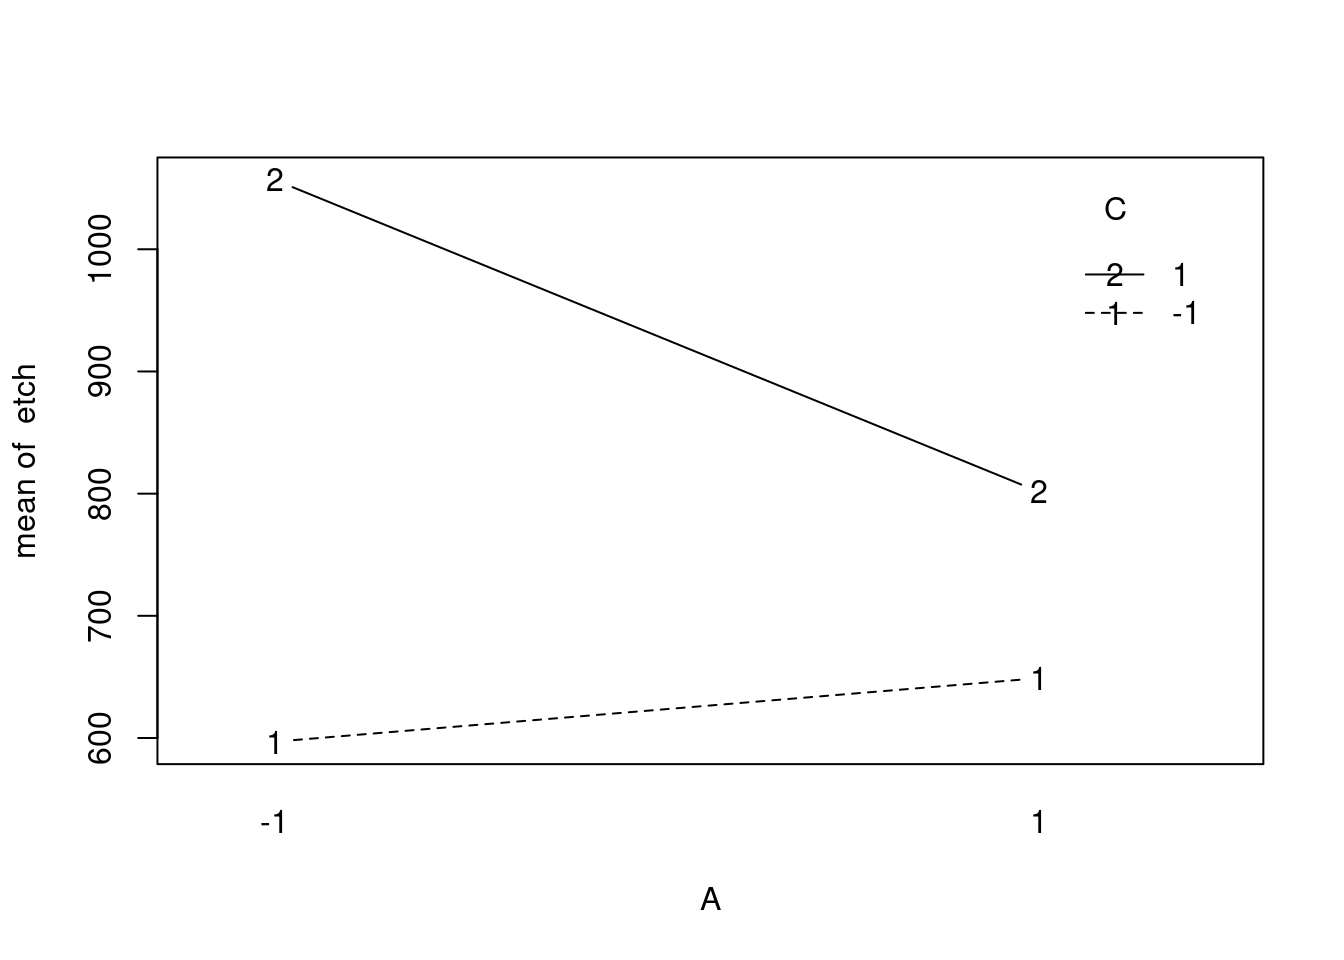
\includegraphics[width=0.8\linewidth]{doe_advanced_files/figure-latex/unnamed-chunk-38-2}

\begin{Shaded}
\begin{Highlighting}[]
\CommentTok{\# The same with ggplot}
\FunctionTok{ggplot}\NormalTok{(plsn, }\FunctionTok{aes}\NormalTok{(}\AttributeTok{x =}\NormalTok{ A, }\AttributeTok{y =}\NormalTok{ etch, }\AttributeTok{fill =}\NormalTok{ C)) }\SpecialCharTok{+}
  \FunctionTok{geom\_boxplot}\NormalTok{()}
\end{Highlighting}
\end{Shaded}

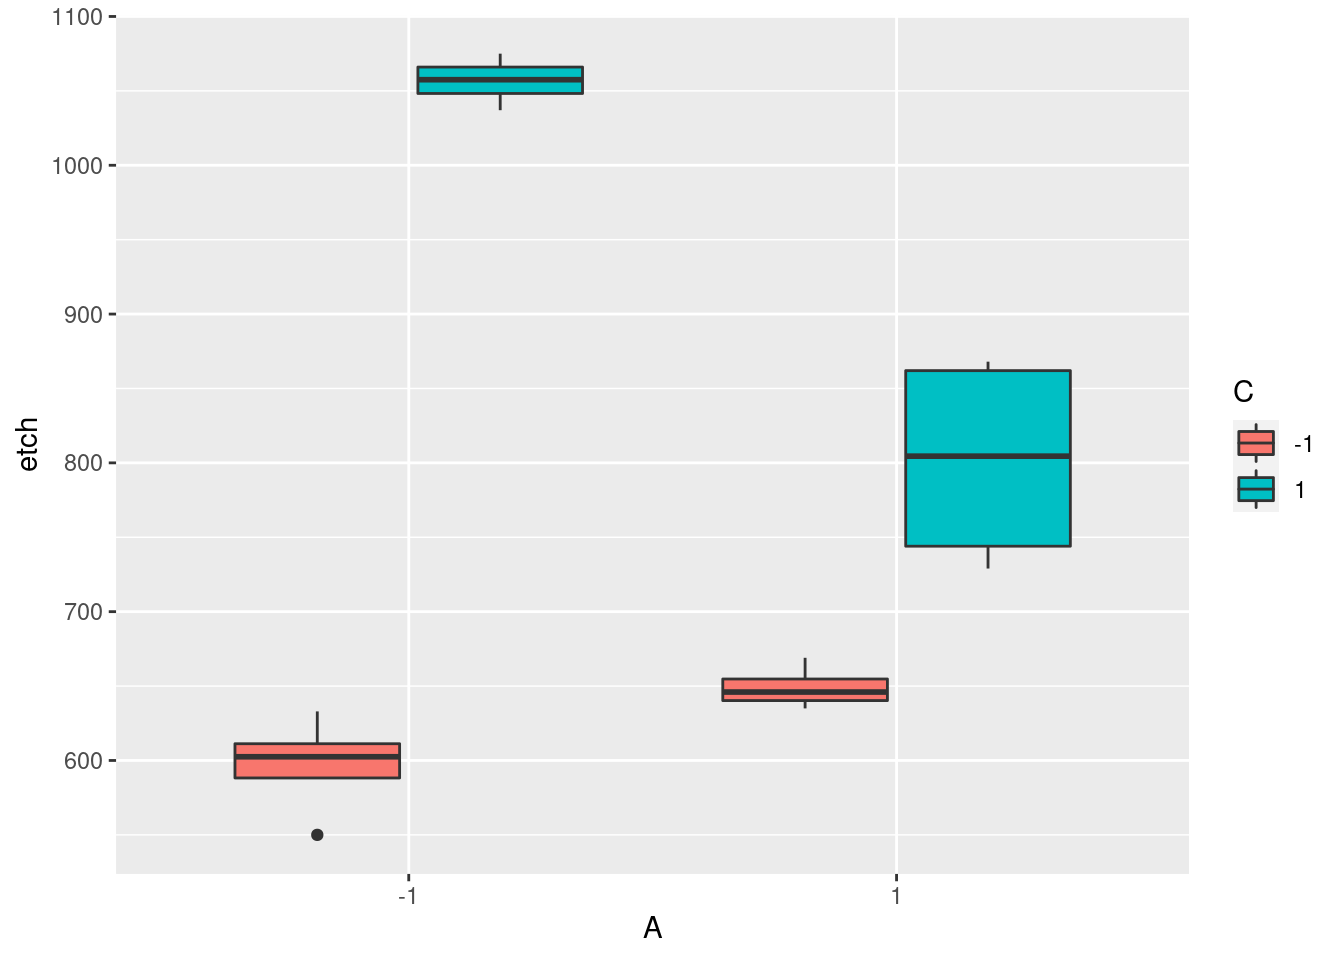
\includegraphics[width=0.8\linewidth]{doe_advanced_files/figure-latex/unnamed-chunk-38-3}

\begin{Shaded}
\begin{Highlighting}[]
\CommentTok{\# Reversed gap {-} power}
\FunctionTok{with}\NormalTok{(plsn, }\FunctionTok{interaction.plot}\NormalTok{(C, A, etch, }\AttributeTok{type =} \StringTok{"b"}\NormalTok{))}
\end{Highlighting}
\end{Shaded}

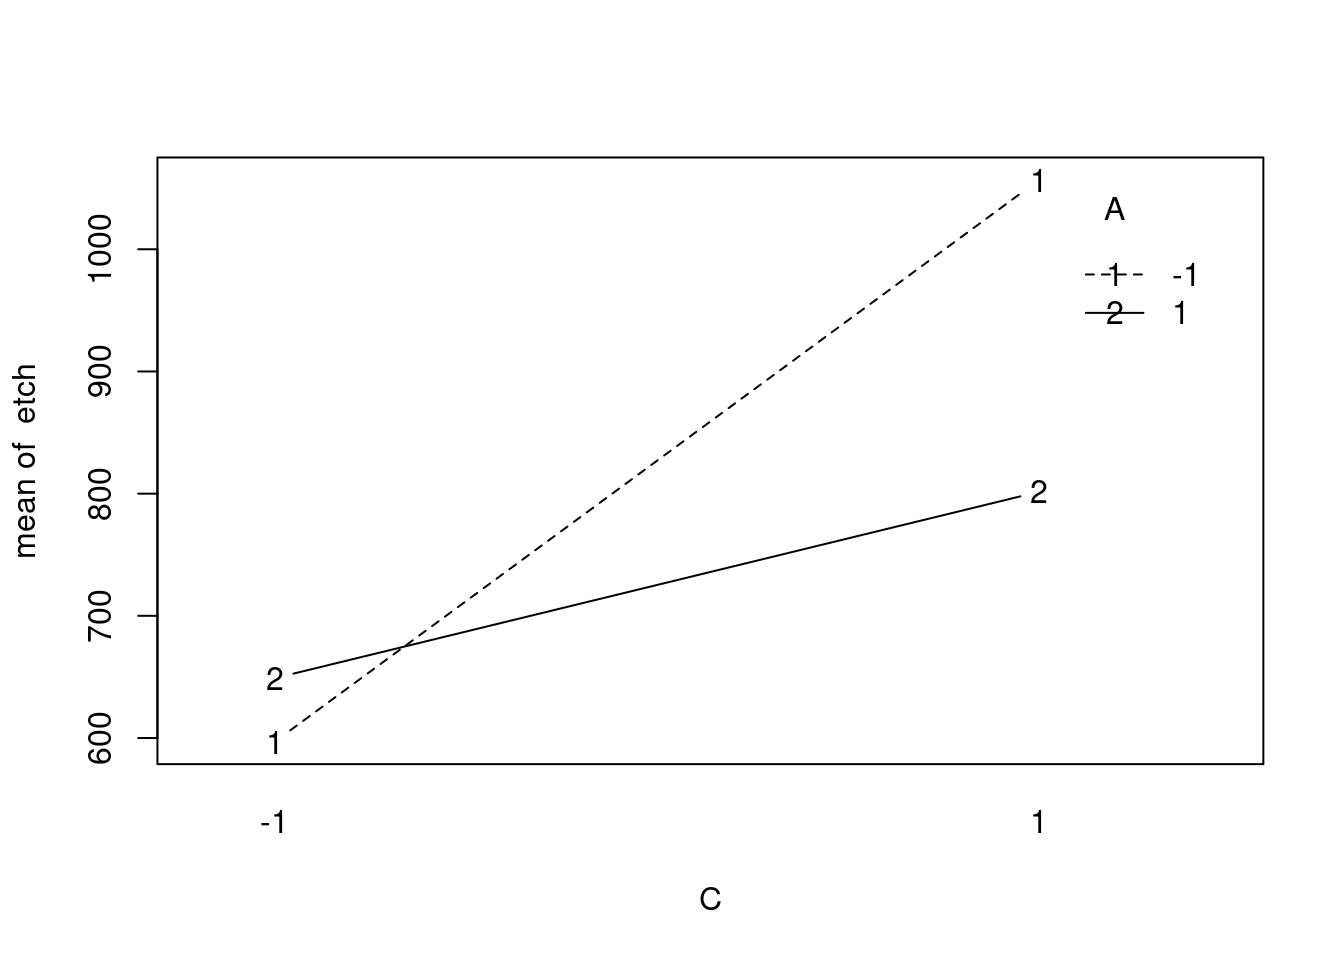
\includegraphics[width=0.8\linewidth]{doe_advanced_files/figure-latex/unnamed-chunk-38-4}

\begin{Shaded}
\begin{Highlighting}[]
\CommentTok{\# The same with ggplot}
\FunctionTok{ggplot}\NormalTok{(plsn, }\FunctionTok{aes}\NormalTok{(}\AttributeTok{x =}\NormalTok{ C, }\AttributeTok{y =}\NormalTok{ etch, }\AttributeTok{fill =}\NormalTok{ A)) }\SpecialCharTok{+}
  \FunctionTok{geom\_boxplot}\NormalTok{()}
\end{Highlighting}
\end{Shaded}

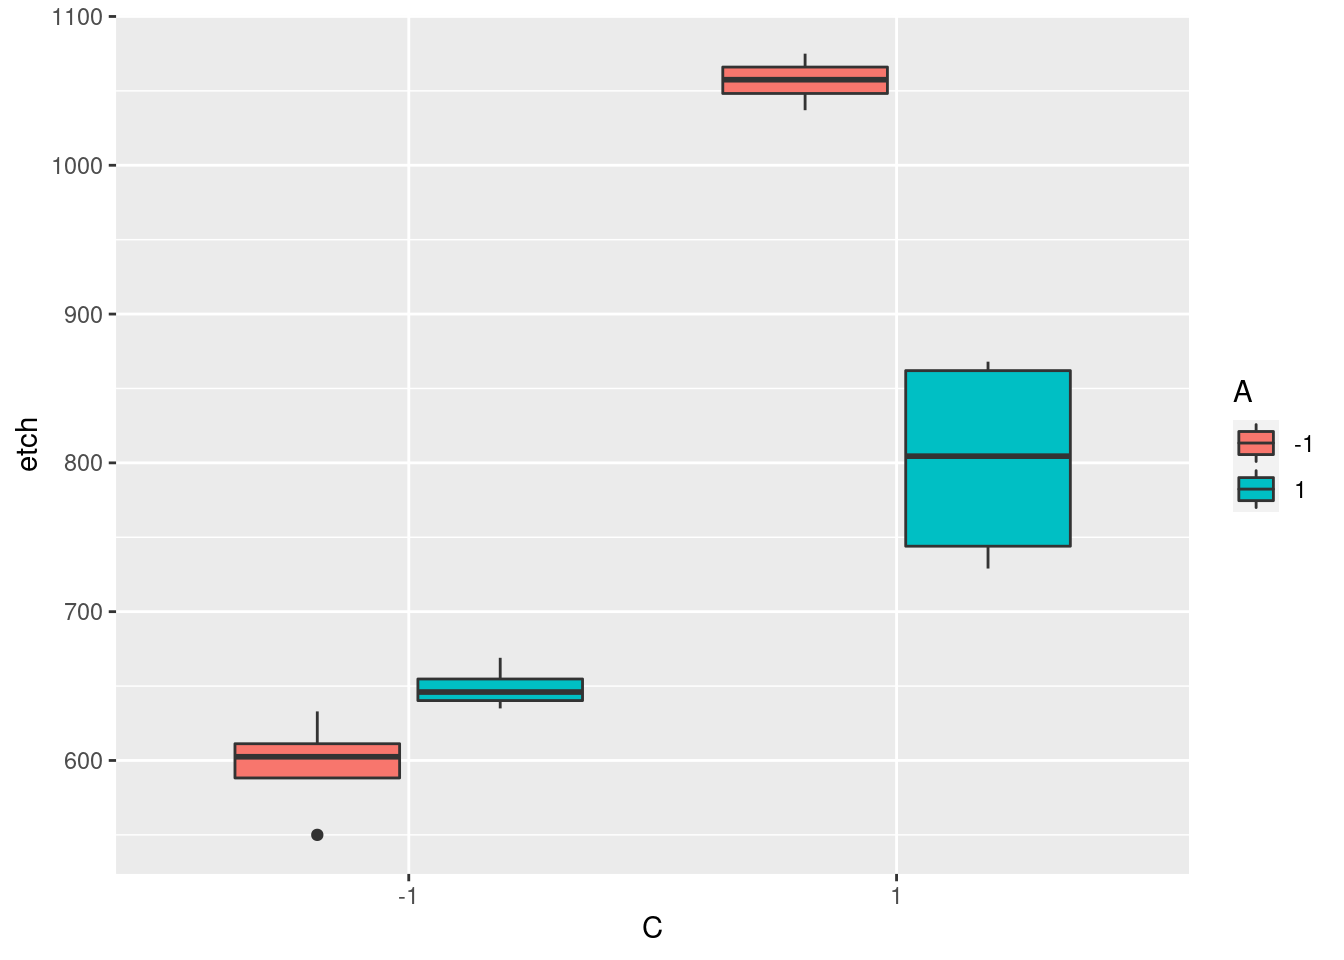
\includegraphics[width=0.8\linewidth]{doe_advanced_files/figure-latex/unnamed-chunk-38-5}

The AC interaction is larger than the main effect of A.
\#\#\# Anova with 1 and -1 factors

\begin{Shaded}
\begin{Highlighting}[]
\NormalTok{plsn\_lm }\OtherTok{\textless{}{-}} \FunctionTok{lm}\NormalTok{(etch }\SpecialCharTok{\textasciitilde{}}\NormalTok{ A }\SpecialCharTok{*}\NormalTok{ B }\SpecialCharTok{*}\NormalTok{ C, plsn)}
\NormalTok{plsn\_aov }\OtherTok{\textless{}{-}} \FunctionTok{aov}\NormalTok{(plsn\_lm)}
\FunctionTok{summary}\NormalTok{(plsn\_aov)}
\end{Highlighting}
\end{Shaded}

\begin{verbatim}
            Df Sum Sq Mean Sq F value   Pr(>F)    
A            1  41311   41311  18.339 0.002679 ** 
B            1    218     218   0.097 0.763911    
C            1 374850  374850 166.411 1.23e-06 ***
A:B          1   2475    2475   1.099 0.325168    
A:C          1  94403   94403  41.909 0.000193 ***
B:C          1     18      18   0.008 0.930849    
A:B:C        1    127     127   0.056 0.818586    
Residuals    8  18020    2253                     
---
Signif. codes:  0 '***' 0.001 '**' 0.01 '*' 0.05 '.' 0.1 ' ' 1
\end{verbatim}

Note here again that the Anova is performed on a model built with the treatments coded as factors, while later the prediction linear model is built with the treatments codes as numeric.
The main effects of Gap and Power are highly significant (both have very small P-values). The AC interaction is also highly significant; thus, there is a strong interaction between Gap and Power.

\hypertarget{converting-levels-to-numeric}{%
\subsection{Converting levels to numeric}\label{converting-levels-to-numeric}}

\begin{Shaded}
\begin{Highlighting}[]
\CommentTok{\# Below the adaptation of the chapter 6.2 approach in converting the factors into numeric, here with tidyverse functions:}
\NormalTok{plsn2 }\OtherTok{\textless{}{-}}\NormalTok{ plsn}
\NormalTok{plsn2 }\OtherTok{\textless{}{-}}\NormalTok{ plsn }\SpecialCharTok{\%\textgreater{}\%} \FunctionTok{mutate}\NormalTok{(}\AttributeTok{cA =} \FunctionTok{ifelse}\NormalTok{(A }\SpecialCharTok{==} \StringTok{"{-}1"}\NormalTok{, }\SpecialCharTok{{-}}\DecValTok{1}\NormalTok{, }\DecValTok{1}\NormalTok{),}
                         \AttributeTok{cB =} \FunctionTok{ifelse}\NormalTok{(B }\SpecialCharTok{==} \StringTok{"{-}1"}\NormalTok{, }\SpecialCharTok{{-}}\DecValTok{1}\NormalTok{, }\DecValTok{1}\NormalTok{),}
                         \AttributeTok{cC =} \FunctionTok{ifelse}\NormalTok{(C }\SpecialCharTok{==} \StringTok{"{-}1"}\NormalTok{, }\SpecialCharTok{{-}}\DecValTok{1}\NormalTok{, }\DecValTok{1}\NormalTok{)}
\NormalTok{                         )}
\end{Highlighting}
\end{Shaded}

\hypertarget{model-with-numeric-levels}{%
\subsection{Model with numeric levels}\label{model-with-numeric-levels}}

\begin{Shaded}
\begin{Highlighting}[]
\NormalTok{plsn2\_lm }\OtherTok{\textless{}{-}} \FunctionTok{lm}\NormalTok{(etch }\SpecialCharTok{\textasciitilde{}}\NormalTok{ cA }\SpecialCharTok{*}\NormalTok{ cB }\SpecialCharTok{*}\NormalTok{ cC, plsn2)}
\FunctionTok{summary}\NormalTok{(plsn2\_lm)}
\end{Highlighting}
\end{Shaded}

\begin{verbatim}
Call:
lm(formula = etch ~ cA * cB * cC, data = plsn2)

Residuals:
   Min     1Q Median     3Q    Max 
-65.50 -11.12   0.00  11.12  65.50 

Coefficients:
            Estimate Std. Error t value Pr(>|t|)    
(Intercept)  776.062     11.865  65.406 3.32e-12 ***
cA           -50.812     11.865  -4.282 0.002679 ** 
cB             3.688     11.865   0.311 0.763911    
cC           153.062     11.865  12.900 1.23e-06 ***
cA:cB        -12.437     11.865  -1.048 0.325168    
cA:cC        -76.812     11.865  -6.474 0.000193 ***
cB:cC         -1.062     11.865  -0.090 0.930849    
cA:cB:cC       2.813     11.865   0.237 0.818586    
---
Signif. codes:  0 '***' 0.001 '**' 0.01 '*' 0.05 '.' 0.1 ' ' 1

Residual standard error: 47.46 on 8 degrees of freedom
Multiple R-squared:  0.9661,	Adjusted R-squared:  0.9364 
F-statistic: 32.56 on 7 and 8 DF,  p-value: 2.896e-05
\end{verbatim}

\hypertarget{prediction-with-numeric-levels}{%
\subsection{Prediction with numeric levels}\label{prediction-with-numeric-levels}}

\begin{Shaded}
\begin{Highlighting}[]
\CommentTok{\# Predict new values}
\NormalTok{plsn\_new }\OtherTok{\textless{}{-}} \FunctionTok{data.frame}\NormalTok{(}\AttributeTok{cA =} \SpecialCharTok{{-}}\DecValTok{1}\NormalTok{, }\AttributeTok{cB =} \DecValTok{1}\NormalTok{, }\AttributeTok{cC =} \DecValTok{1}\NormalTok{)}
\FunctionTok{predict}\NormalTok{(plsn2\_lm, }\AttributeTok{newdata =}\NormalTok{ plsn\_new)}
\end{Highlighting}
\end{Shaded}

\begin{verbatim}
   1 
1069 
\end{verbatim}

\begin{Shaded}
\begin{Highlighting}[]
\CommentTok{\# Compare with predicted table below (the same values are found!)}
\NormalTok{plsn2\_tidy }\OtherTok{\textless{}{-}} \FunctionTok{augment}\NormalTok{(plsn2\_lm)}
\end{Highlighting}
\end{Shaded}

The linear model coeficients obtained correspond to the book example.
The predict function correctly corresponds to the predictions obtained with the augment function.

The ordinary R\^{}2 is 0.9661 and it measures the proportion of total variability explained by the model. A potential problem with this statistic is that it always increases as factors are added to the model, even if these factors are not significant. The adjusted R\^{}2 is obtained by dividing the Sums of Squares by the degrees of freedom, and is adjusted for the size of the model, that is the number of factors.

\hypertarget{reduced-model-removing-levels}{%
\subsection{Reduced model (removing levels)}\label{reduced-model-removing-levels}}

\begin{Shaded}
\begin{Highlighting}[]
\NormalTok{plsn3\_lm }\OtherTok{\textless{}{-}} \FunctionTok{lm}\NormalTok{(etch }\SpecialCharTok{\textasciitilde{}}\NormalTok{ cA }\SpecialCharTok{+}\NormalTok{ cC }\SpecialCharTok{+}\NormalTok{ cA}\SpecialCharTok{:}\NormalTok{cC, plsn2)}
\FunctionTok{summary}\NormalTok{(plsn3\_lm)}
\end{Highlighting}
\end{Shaded}

\begin{verbatim}
Call:
lm(formula = etch ~ cA + cC + cA:cC, data = plsn2)

Residuals:
   Min     1Q Median     3Q    Max 
-72.50 -15.44   2.50  18.69  66.50 

Coefficients:
            Estimate Std. Error t value Pr(>|t|)    
(Intercept)   776.06      10.42  74.458  < 2e-16 ***
cA            -50.81      10.42  -4.875 0.000382 ***
cC            153.06      10.42  14.685 4.95e-09 ***
cA:cC         -76.81      10.42  -7.370 8.62e-06 ***
---
Signif. codes:  0 '***' 0.001 '**' 0.01 '*' 0.05 '.' 0.1 ' ' 1

Residual standard error: 41.69 on 12 degrees of freedom
Multiple R-squared:  0.9608,	Adjusted R-squared:  0.9509 
F-statistic: 97.91 on 3 and 12 DF,  p-value: 1.054e-08
\end{verbatim}

Adjusted R² has improved! Clearly, removing the nonsignificant terms from the full model has produced a final model that is likely to function more effectively as a predictor of new data!

\hypertarget{k-factorial-design}{%
\section{2\^{}k factorial design}\label{k-factorial-design}}

\hypertarget{combinations}{%
\subsection{Combinations}\label{combinations}}

\begin{Shaded}
\begin{Highlighting}[]
\NormalTok{a }\OtherTok{\textless{}{-}} \DecValTok{2}   \CommentTok{\# levels}
\NormalTok{k }\OtherTok{\textless{}{-}} \DecValTok{4}   \CommentTok{\# degrees of freedom (to which factors can be associated)}
\NormalTok{trials }\OtherTok{\textless{}{-}}\NormalTok{ a}\SpecialCharTok{\^{}}\NormalTok{k}
\NormalTok{trials}
\end{Highlighting}
\end{Shaded}

\begin{verbatim}
[1] 16
\end{verbatim}

\begin{Shaded}
\begin{Highlighting}[]
\NormalTok{n }\OtherTok{\textless{}{-}} \DecValTok{2}   \CommentTok{\# replications (repetitions of each trial)}
\NormalTok{runs }\OtherTok{\textless{}{-}}\NormalTok{ a}\SpecialCharTok{\^{}}\NormalTok{k}\SpecialCharTok{*}\NormalTok{n }\CommentTok{\# actual number of individual tests to be done}
\NormalTok{runs}
\end{Highlighting}
\end{Shaded}

\begin{verbatim}
[1] 32
\end{verbatim}

Analysis Procedure for a 2 k Design

\begin{enumerate}
\def\labelenumi{\arabic{enumi}.}
\tightlist
\item
  Estimate factor effects
\item
  Form initial model (full model)
\end{enumerate}

\begin{enumerate}
\def\labelenumi{\alph{enumi}.}
\tightlist
\item
  If the design is replicated, fit the full model
\item
  If there is no replication, form the model using a normal probability plot of the effects
\end{enumerate}

\begin{enumerate}
\def\labelenumi{\arabic{enumi}.}
\setcounter{enumi}{2}
\tightlist
\item
  Perform statistical testing (Anova)
\item
  Refine model (remove non significant effects)
\item
  Analyze residuals
\item
  Interpret results
\end{enumerate}

DEF - Sparsity of effects principle: most systems are dominated by some of the main effects and low-order interactions, and most high-order interactions are negligible.

\hypertarget{coded-vs-natural-variables}{%
\subsection{Coded vs natural variables}\label{coded-vs-natural-variables}}

\begin{Shaded}
\begin{Highlighting}[]
\CommentTok{\# Converting absolute value Ax into coded value Ai:}
\NormalTok{Al }\OtherTok{\textless{}{-}} \DecValTok{15}
\NormalTok{Ah }\OtherTok{\textless{}{-}} \DecValTok{25}
\NormalTok{Ax }\OtherTok{\textless{}{-}} \DecValTok{16}

\NormalTok{Ai }\OtherTok{\textless{}{-}}\NormalTok{ (Ax }\SpecialCharTok{{-}}\NormalTok{ (Al }\SpecialCharTok{+}\NormalTok{ Ah) }\SpecialCharTok{/} \DecValTok{2}\NormalTok{) }\SpecialCharTok{/}\NormalTok{ ((Ah }\SpecialCharTok{{-}}\NormalTok{  Al ) }\SpecialCharTok{/} \DecValTok{2}\NormalTok{)}
\NormalTok{Ai}
\end{Highlighting}
\end{Shaded}

\begin{verbatim}
[1] -0.8
\end{verbatim}

\begin{Shaded}
\begin{Highlighting}[]
\CommentTok{\# Converting coded value Bi into absolute value Bx}
\NormalTok{Bl }\OtherTok{\textless{}{-}} \DecValTok{15}
\NormalTok{Bh }\OtherTok{\textless{}{-}} \DecValTok{25}
\NormalTok{Bi }\OtherTok{\textless{}{-}} \SpecialCharTok{{-}}\FloatTok{0.8}

\NormalTok{Bx }\OtherTok{\textless{}{-}}\NormalTok{ Bi }\SpecialCharTok{*}\NormalTok{ ((Bh }\SpecialCharTok{{-}}\NormalTok{ Bl) }\SpecialCharTok{/} \DecValTok{2}\NormalTok{) }\SpecialCharTok{+}\NormalTok{ ((Bl }\SpecialCharTok{+}\NormalTok{ Bh)}\SpecialCharTok{/}\DecValTok{2}\NormalTok{)}
\NormalTok{Bx}
\end{Highlighting}
\end{Shaded}

\begin{verbatim}
[1] 16
\end{verbatim}

\hypertarget{k-single-replicate-design}{%
\section{2\^{}k single replicate design}\label{k-single-replicate-design}}

Possible approaches
- assume some high-order interactions are zero, and fit a model that excludes them; degrees of freedom go into error, so testing is possible (not recommended)
- graphical methods--normal and half-normal probability plots; no formal tests;

The Filtration example

\begin{Shaded}
\begin{Highlighting}[]
\NormalTok{flt }\OtherTok{\textless{}{-}} \FunctionTok{read.csv}\NormalTok{(}\StringTok{"../industRial/data{-}raw/6{-}4\_filtration.csv"}\NormalTok{)}
\CommentTok{\# Below a replacement of the individual conversion of each treatment into a factor, now with the lapply function. This is scalable to any number of factors.}
\NormalTok{flt2 }\OtherTok{\textless{}{-}} \FunctionTok{lapply}\NormalTok{(}\AttributeTok{X =}\NormalTok{ flt[,}\DecValTok{1}\SpecialCharTok{:}\DecValTok{4}\NormalTok{], }\AttributeTok{FUN =}\NormalTok{ as.factor)}
\NormalTok{flt2 }\OtherTok{\textless{}{-}} \FunctionTok{bind\_rows}\NormalTok{(flt2)}
\NormalTok{flt2 }\OtherTok{\textless{}{-}} \FunctionTok{mutate}\NormalTok{(flt2, }\AttributeTok{filtration =}\NormalTok{ flt}\SpecialCharTok{$}\NormalTok{filtration)}
\end{Highlighting}
\end{Shaded}

\hypertarget{main-effects-data-plots}{%
\subsection{Main effects data plots}\label{main-effects-data-plots}}

Factors (reminder)
A - Temperature
B - Pressure
C - Concentration
D - Stirring

\begin{Shaded}
\begin{Highlighting}[]
\FunctionTok{ggplot}\NormalTok{(flt2, }\FunctionTok{aes}\NormalTok{(}\AttributeTok{x =}\NormalTok{ A, }\AttributeTok{y =}\NormalTok{ filtration)) }\SpecialCharTok{+}
  \FunctionTok{geom\_boxplot}\NormalTok{()}
\end{Highlighting}
\end{Shaded}

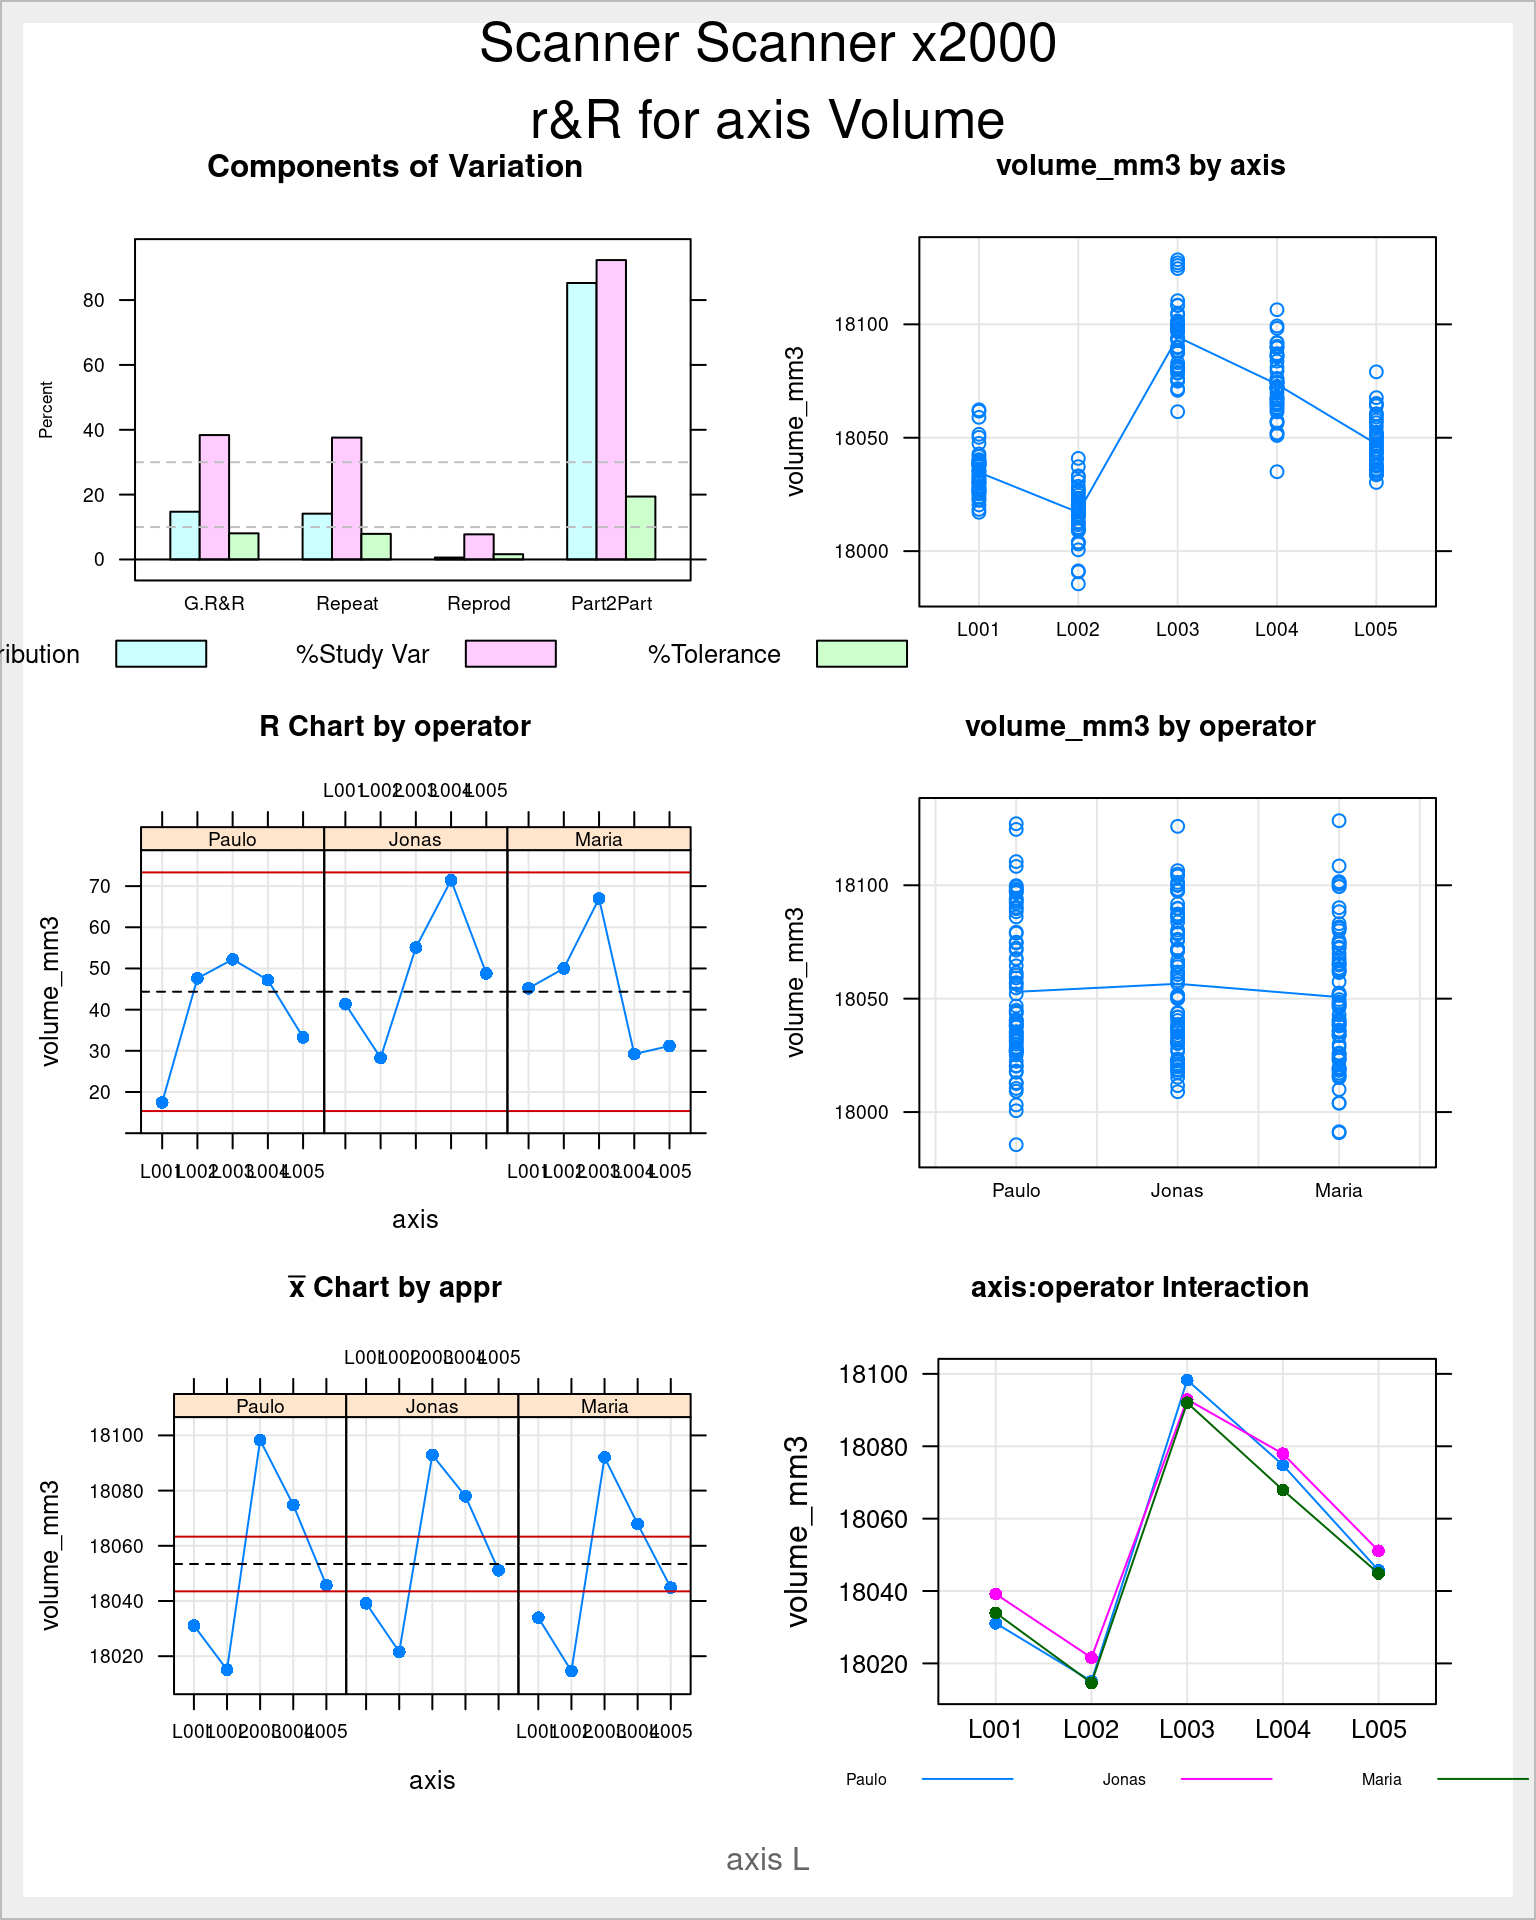
\includegraphics[width=0.8\linewidth]{doe_advanced_files/figure-latex/unnamed-chunk-47-1}

\begin{Shaded}
\begin{Highlighting}[]
\FunctionTok{ggplot}\NormalTok{(flt2, }\FunctionTok{aes}\NormalTok{(}\AttributeTok{x =}\NormalTok{ C, }\AttributeTok{y =}\NormalTok{ filtration)) }\SpecialCharTok{+}
  \FunctionTok{geom\_boxplot}\NormalTok{()}
\end{Highlighting}
\end{Shaded}

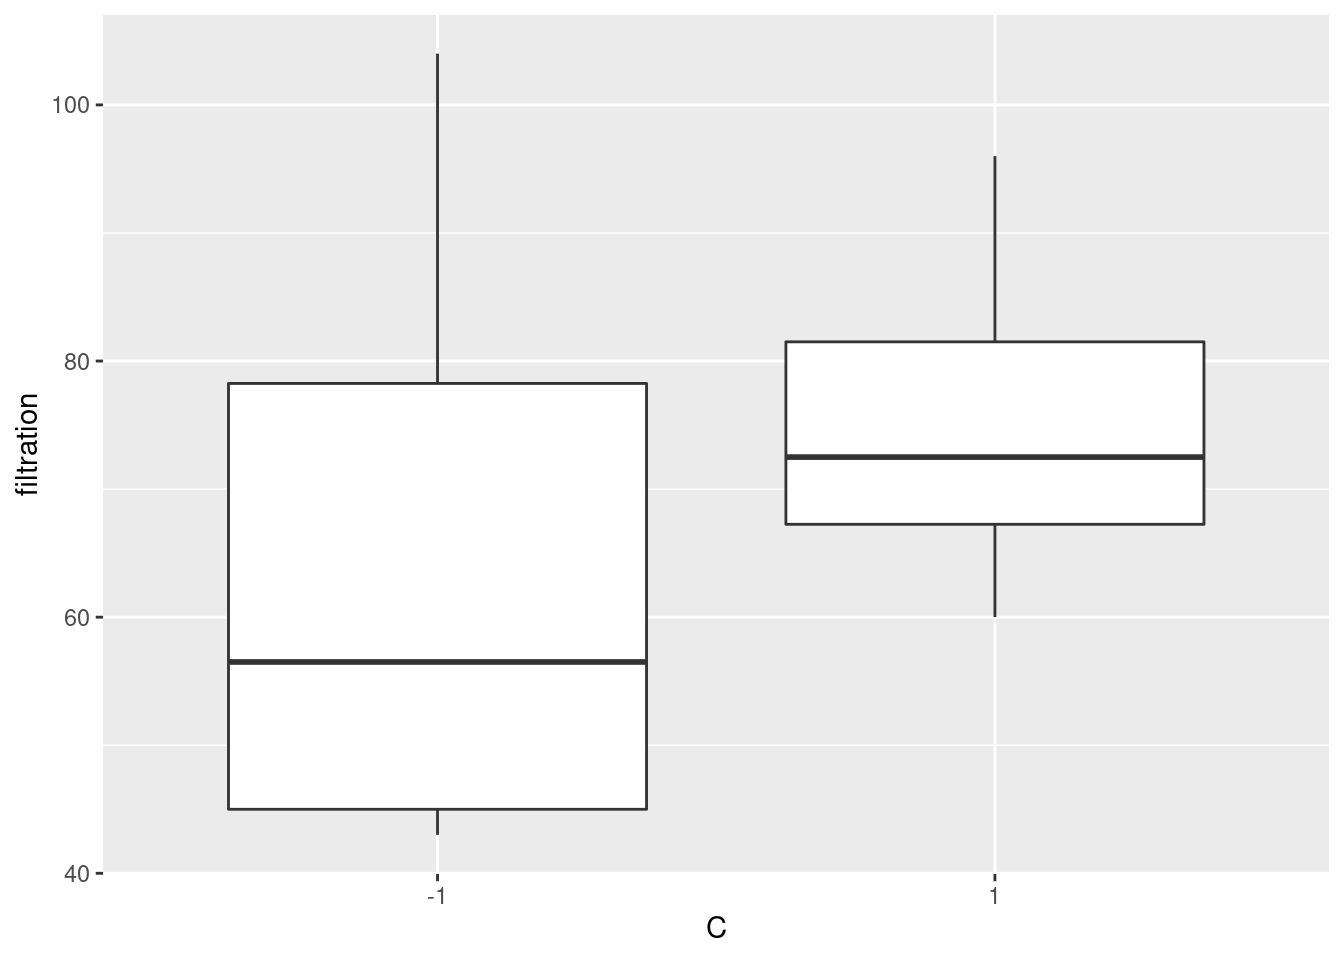
\includegraphics[width=0.8\linewidth]{doe_advanced_files/figure-latex/unnamed-chunk-47-2}

\begin{Shaded}
\begin{Highlighting}[]
\FunctionTok{ggplot}\NormalTok{(flt2, }\FunctionTok{aes}\NormalTok{(}\AttributeTok{x =}\NormalTok{ D, }\AttributeTok{y =}\NormalTok{ filtration)) }\SpecialCharTok{+}
  \FunctionTok{geom\_boxplot}\NormalTok{()}
\end{Highlighting}
\end{Shaded}

\includegraphics[width=0.8\linewidth]{doe_advanced_files/figure-latex/unnamed-chunk-47-3}

\begin{Shaded}
\begin{Highlighting}[]
\FunctionTok{ggplot}\NormalTok{(flt2, }\FunctionTok{aes}\NormalTok{(}\AttributeTok{x =}\NormalTok{ A, }\AttributeTok{y =}\NormalTok{ filtration, }\AttributeTok{fill =}\NormalTok{ C)) }\SpecialCharTok{+}
  \FunctionTok{geom\_boxplot}\NormalTok{()}
\end{Highlighting}
\end{Shaded}

\includegraphics[width=0.8\linewidth]{doe_advanced_files/figure-latex/unnamed-chunk-47-4}

\begin{Shaded}
\begin{Highlighting}[]
\FunctionTok{ggplot}\NormalTok{(flt2, }\FunctionTok{aes}\NormalTok{(}\AttributeTok{x =}\NormalTok{ A, }\AttributeTok{y =}\NormalTok{ filtration, }\AttributeTok{fill =}\NormalTok{ D)) }\SpecialCharTok{+}
  \FunctionTok{geom\_boxplot}\NormalTok{()}
\end{Highlighting}
\end{Shaded}

\includegraphics[width=0.8\linewidth]{doe_advanced_files/figure-latex/unnamed-chunk-47-5}

The AC and AD interactions are plotted in Figure 6.12b. These interactions are the key to solving the problem. Note from the AC interaction that the temperature effect is very small when the concentration is at the high level and very large when the concentration is at the low level, with the best results obtained with low concentration and high temperature. The AD interaction indicates that stirring rate D has little effect at low temperature but a large positive effect at high temperature. Therefore, the best filtration rates would appear to be obtained when A and D are at the high level and C is at the low level. This would allow the reduction of the formaldehyde concentration to a lower level, another objective of the experimenter.

\hypertarget{linear-model-single-replicate}{%
\subsection{Linear model single replicate}\label{linear-model-single-replicate}}

\begin{Shaded}
\begin{Highlighting}[]
\NormalTok{flt2\_lm }\OtherTok{\textless{}{-}} \FunctionTok{lm}\NormalTok{(filtration }\SpecialCharTok{\textasciitilde{}}\NormalTok{ A }\SpecialCharTok{*}\NormalTok{ B }\SpecialCharTok{*}\NormalTok{ C }\SpecialCharTok{*}\NormalTok{ D, flt2)}
\end{Highlighting}
\end{Shaded}

\hypertarget{anova-single-replicate}{%
\subsection{Anova single replicate}\label{anova-single-replicate}}

\begin{Shaded}
\begin{Highlighting}[]
\NormalTok{flt2\_aov }\OtherTok{\textless{}{-}} \FunctionTok{aov}\NormalTok{(flt2\_lm)}
\FunctionTok{summary}\NormalTok{(flt2\_aov)}
\end{Highlighting}
\end{Shaded}

\begin{verbatim}
            Df Sum Sq Mean Sq
A            1 1870.6  1870.6
B            1   39.1    39.1
C            1  390.1   390.1
D            1  855.6   855.6
A:B          1    0.1     0.1
A:C          1 1314.1  1314.1
B:C          1   22.6    22.6
A:D          1 1105.6  1105.6
B:D          1    0.6     0.6
C:D          1    5.1     5.1
A:B:C        1   14.1    14.1
A:B:D        1   68.1    68.1
A:C:D        1   10.6    10.6
B:C:D        1   27.6    27.6
A:B:C:D      1    7.6     7.6
\end{verbatim}

My understanding is that since only 1 replicate has been done there is no statistical testing, thus no p values.

\hypertarget{linear-regression---plot-of-effects}{%
\subsection{Linear regression - Plot of effects}\label{linear-regression---plot-of-effects}}

\begin{Shaded}
\begin{Highlighting}[]
\CommentTok{\# The effect estimates have to be extracted from the lm of the data, not in factors, from the coefficients vector...}
\NormalTok{flt\_lm }\OtherTok{\textless{}{-}} \FunctionTok{lm}\NormalTok{(filtration }\SpecialCharTok{\textasciitilde{}}\NormalTok{ A }\SpecialCharTok{*}\NormalTok{ B }\SpecialCharTok{*}\NormalTok{ C }\SpecialCharTok{*}\NormalTok{ D, flt)}
\NormalTok{flt\_eff }\OtherTok{\textless{}{-}}\NormalTok{ (flt\_lm}\SpecialCharTok{$}\NormalTok{coefficients)[}\DecValTok{2}\SpecialCharTok{:}\DecValTok{16}\NormalTok{]}
\NormalTok{flt\_eff\_names }\OtherTok{\textless{}{-}} \FunctionTok{names}\NormalTok{((flt\_lm}\SpecialCharTok{$}\NormalTok{coefficients)[}\DecValTok{2}\SpecialCharTok{:}\DecValTok{16}\NormalTok{])}

\FunctionTok{qqnorm}\NormalTok{(flt\_eff, }\AttributeTok{datax =} \ConstantTok{TRUE}\NormalTok{); }\FunctionTok{qqline}\NormalTok{(flt\_eff, }\AttributeTok{datax =} \ConstantTok{TRUE}\NormalTok{)}
\end{Highlighting}
\end{Shaded}

\includegraphics[width=0.8\linewidth]{doe_advanced_files/figure-latex/unnamed-chunk-50-1}

\begin{Shaded}
\begin{Highlighting}[]
\CommentTok{\# Replacement of base R plot by a tidyverse plot with ggplot2}
\CommentTok{\# (to be explored further how to add the labels to the graph)}
\NormalTok{flt\_eff\_df }\OtherTok{\textless{}{-}} \FunctionTok{data.frame}\NormalTok{(flt\_eff\_names, flt\_eff, }\AttributeTok{row.names =} \ConstantTok{NULL}\NormalTok{)}
\FunctionTok{ggplot}\NormalTok{(flt\_eff\_df, }\FunctionTok{aes}\NormalTok{(}\AttributeTok{sample =}\NormalTok{ flt\_eff)) }\SpecialCharTok{+} 
    \FunctionTok{stat\_qq}\NormalTok{() }\SpecialCharTok{+}
    \FunctionTok{stat\_qq\_line}\NormalTok{() }\SpecialCharTok{+}
    \FunctionTok{coord\_flip}\NormalTok{()}
\end{Highlighting}
\end{Shaded}

\includegraphics[width=0.8\linewidth]{doe_advanced_files/figure-latex/unnamed-chunk-51-1}

\begin{Shaded}
\begin{Highlighting}[]
\CommentTok{\# Anyway a better plot from the car package (already loaded in this Rmd) if the qqPlot.}
\FunctionTok{qqPlot}\NormalTok{(flt\_eff, }\AttributeTok{envelope =} \FloatTok{0.70}\NormalTok{, }
       \AttributeTok{id =} \FunctionTok{list}\NormalTok{(}\AttributeTok{method=}\StringTok{"y"}\NormalTok{, }\AttributeTok{n=}\DecValTok{5}\NormalTok{, }\AttributeTok{cex=}\DecValTok{1}\NormalTok{, }\AttributeTok{col=}\FunctionTok{carPalette}\NormalTok{()[}\DecValTok{1}\NormalTok{], }\AttributeTok{location=}\StringTok{"lr"}\NormalTok{), }
       \AttributeTok{grid =} \ConstantTok{FALSE}\NormalTok{)}
\end{Highlighting}
\end{Shaded}

\includegraphics[width=0.8\linewidth]{doe_advanced_files/figure-latex/unnamed-chunk-51-2}

\begin{verbatim}
A:C   A A:D   D   C 
  6   1   8   4   3 
\end{verbatim}

In this case it may take long to be able to reproduce this example.
The important effects that emerge from this analysis are the main effects of A, C, and D and the AC and AD interactions.
The last plot shows that this method of selecting the significant effects is rather subjective as it is stated by Montgomery. To go deeper on a more objective method see Lenth's method.

\hypertarget{anova-reduced-model-significant-effects-only}{%
\subsection{Anova reduced model (significant effects only)}\label{anova-reduced-model-significant-effects-only}}

Since the B factor has little influence on the output it can be removed from the model.

\begin{Shaded}
\begin{Highlighting}[]
\NormalTok{flt3\_lm }\OtherTok{\textless{}{-}} \FunctionTok{lm}\NormalTok{(filtration }\SpecialCharTok{\textasciitilde{}}\NormalTok{ A }\SpecialCharTok{*}\NormalTok{ C }\SpecialCharTok{*}\NormalTok{ D, flt2)}
\NormalTok{flt3\_aov }\OtherTok{\textless{}{-}} \FunctionTok{aov}\NormalTok{(flt3\_lm)}
\FunctionTok{summary}\NormalTok{(flt3\_aov)}
\end{Highlighting}
\end{Shaded}

\begin{verbatim}
            Df Sum Sq Mean Sq F value   Pr(>F)    
A            1 1870.6  1870.6  83.368 1.67e-05 ***
C            1  390.1   390.1  17.384 0.003124 ** 
D            1  855.6   855.6  38.131 0.000267 ***
A:C          1 1314.1  1314.1  58.565 6.00e-05 ***
A:D          1 1105.6  1105.6  49.273 0.000110 ***
C:D          1    5.1     5.1   0.226 0.647483    
A:C:D        1   10.6    10.6   0.471 0.512032    
Residuals    8  179.5    22.4                     
---
Signif. codes:  0 '***' 0.001 '**' 0.01 '*' 0.05 '.' 0.1 ' ' 1
\end{verbatim}

\hypertarget{reduced-model}{%
\subsection{Reduced model}\label{reduced-model}}

\begin{Shaded}
\begin{Highlighting}[]
\CommentTok{\# on the reduced model, on specific effects and interactions, not as factors:}
\NormalTok{flt4\_lm }\OtherTok{\textless{}{-}} \FunctionTok{lm}\NormalTok{(filtration }\SpecialCharTok{\textasciitilde{}}\NormalTok{ (A }\SpecialCharTok{+}\NormalTok{ C }\SpecialCharTok{+}\NormalTok{ D }\SpecialCharTok{+}\NormalTok{ A}\SpecialCharTok{:}\NormalTok{C }\SpecialCharTok{+}\NormalTok{ A}\SpecialCharTok{:}\NormalTok{D), flt)}
\FunctionTok{summary}\NormalTok{(flt4\_lm)}
\end{Highlighting}
\end{Shaded}

\begin{verbatim}
Call:
lm(formula = filtration ~ (A + C + D + A:C + A:D), data = flt)

Residuals:
    Min      1Q  Median      3Q     Max 
-6.3750 -1.5000  0.0625  2.9062  5.7500 

Coefficients:
            Estimate Std. Error t value Pr(>|t|)    
(Intercept)   70.062      1.104  63.444 2.30e-14 ***
A             10.812      1.104   9.791 1.93e-06 ***
C              4.938      1.104   4.471   0.0012 ** 
D              7.313      1.104   6.622 5.92e-05 ***
A:C           -9.063      1.104  -8.206 9.41e-06 ***
A:D            8.312      1.104   7.527 2.00e-05 ***
---
Signif. codes:  0 '***' 0.001 '**' 0.01 '*' 0.05 '.' 0.1 ' ' 1

Residual standard error: 4.417 on 10 degrees of freedom
Multiple R-squared:  0.966,	Adjusted R-squared:  0.9489 
F-statistic: 56.74 on 5 and 10 DF,  p-value: 5.14e-07
\end{verbatim}

\begin{Shaded}
\begin{Highlighting}[]
\NormalTok{flt4\_eff }\OtherTok{\textless{}{-}}\NormalTok{ (flt4\_lm}\SpecialCharTok{$}\NormalTok{coefficients)[}\DecValTok{2}\SpecialCharTok{:}\DecValTok{16}\NormalTok{]}
\NormalTok{flt4\_eff}
\end{Highlighting}
\end{Shaded}

\begin{verbatim}
      A       C       D     A:C     A:D    <NA>    <NA>    <NA>    <NA>    <NA> 
10.8125  4.9375  7.3125 -9.0625  8.3125      NA      NA      NA      NA      NA 
   <NA>    <NA>    <NA>    <NA>    <NA> 
     NA      NA      NA      NA      NA 
\end{verbatim}

\begin{Shaded}
\begin{Highlighting}[]
\NormalTok{flt\_new }\OtherTok{\textless{}{-}} \FunctionTok{data.frame}\NormalTok{(}\AttributeTok{A =} \SpecialCharTok{{-}}\DecValTok{1}\NormalTok{, }\AttributeTok{C =} \SpecialCharTok{{-}}\DecValTok{1}\NormalTok{, }\AttributeTok{D =} \SpecialCharTok{{-}}\DecValTok{1}\NormalTok{)}
\FunctionTok{predict}\NormalTok{(flt4\_lm, }\AttributeTok{newdata =}\NormalTok{ flt\_new)}
\end{Highlighting}
\end{Shaded}

\begin{verbatim}
    1 
46.25 
\end{verbatim}

\begin{Shaded}
\begin{Highlighting}[]
\NormalTok{flt4\_tidy }\OtherTok{\textless{}{-}} \FunctionTok{augment}\NormalTok{(flt4\_lm) }\CommentTok{\# as page 261 of the book}
\end{Highlighting}
\end{Shaded}

\hypertarget{reduced-model-check}{%
\subsection{Reduced model check}\label{reduced-model-check}}

\begin{Shaded}
\begin{Highlighting}[]
\FunctionTok{qqnorm}\NormalTok{(flt4\_lm}\SpecialCharTok{$}\NormalTok{residuals, }\AttributeTok{datax =} \ConstantTok{TRUE}\NormalTok{);}\FunctionTok{qqline}\NormalTok{(flt4\_lm}\SpecialCharTok{$}\NormalTok{residuals, }\AttributeTok{datax =} \ConstantTok{TRUE}\NormalTok{)}
\end{Highlighting}
\end{Shaded}

\includegraphics[width=0.8\linewidth]{doe_advanced_files/figure-latex/unnamed-chunk-54-1}

\hypertarget{MSA}{%
\chapter{MSA - Measurement System Analysis}\label{MSA}}

Validation of a measurement device

\hypertarget{robustness}{%
\section{Robustness}\label{robustness}}

In the Six Sigma chapter we presented the Ishikawa diagram \ref{fig:fig-ishikawa}. The identification of the factors for which to verify a measurement system robustness is a typical case where we can make good use of such tool and properly list the environmental factors that may influence the measurement.

\hypertarget{linearity}{%
\section{Linearity}\label{linearity}}

The Quality Control Manager of a Juice producing plant acquired a faster dry matter content measurement device from the supplier DRX. An important reduction of the control time was the rational for the acquisition and now before finally putting it into operation its performance is being assessed and validated.

\begin{figure}

{\centering \includegraphics[width=0.6\linewidth]{img/juice_bottling_bw} 

}

\caption{juice bottling line}\label{fig:unnamed-chunk-2}
\end{figure}

In this case study we will look into the assessment of the linearity which is the difference in average bias throughout the measurement range.

Dry matter content for the company top seller juices have around 12\% dry matter as for example Premium Fresh Apple juice: 12.4 \% and Austrian Beetroot: 13.2\% and some other specialities may have a higher content up such as Organic Carrot with 16.3\%.

It has been decided to start by checking the equipement in the range of 10 to 20\% dry matter content.

\begin{Shaded}
\begin{Highlighting}[]
\FunctionTok{library}\NormalTok{(tidyverse)}
\FunctionTok{library}\NormalTok{(readxl)}
\FunctionTok{library}\NormalTok{(janitor)}
\FunctionTok{library}\NormalTok{(stats)}
\FunctionTok{library}\NormalTok{(knitr)}
\NormalTok{filter }\OtherTok{\textless{}{-}}\NormalTok{ dplyr}\SpecialCharTok{::}\NormalTok{filter}
\NormalTok{select }\OtherTok{\textless{}{-}}\NormalTok{ dplyr}\SpecialCharTok{::}\NormalTok{select}
\end{Highlighting}
\end{Shaded}

Data loading

\begin{Shaded}
\begin{Highlighting}[]
\NormalTok{juices }\OtherTok{\textless{}{-}} \FunctionTok{read\_excel}\NormalTok{(}\AttributeTok{path =} \StringTok{"../industRial/data{-}raw/juices.xlsx"}\NormalTok{) }

\NormalTok{juices }\OtherTok{\textless{}{-}}\NormalTok{ juices }\SpecialCharTok{\%\textgreater{}\%}
  \FunctionTok{mutate}\NormalTok{(}\AttributeTok{bias =}\NormalTok{ DRX }\SpecialCharTok{{-}}\NormalTok{ Ref)}
\end{Highlighting}
\end{Shaded}

\hypertarget{plot-of-bias-data}{%
\subsection{Plot of bias data}\label{plot-of-bias-data}}

\begin{Shaded}
\begin{Highlighting}[]
\NormalTok{juices }\SpecialCharTok{\%\textgreater{}\%}
  \FunctionTok{ggplot}\NormalTok{(}\FunctionTok{aes}\NormalTok{(}\AttributeTok{x =}\NormalTok{ Ref, }\AttributeTok{y =}\NormalTok{ bias)) }\SpecialCharTok{+}
  \FunctionTok{geom\_point}\NormalTok{() }\SpecialCharTok{+}
  \FunctionTok{geom\_smooth}\NormalTok{(}\AttributeTok{method =} \StringTok{"lm"}\NormalTok{, }\AttributeTok{se =}\NormalTok{ T, ) }\SpecialCharTok{+}
  \FunctionTok{theme\_light}\NormalTok{() }\SpecialCharTok{+}
  \CommentTok{\# facet\_grid(\textasciitilde{}dissolution) +}
  \FunctionTok{labs}\NormalTok{(}\AttributeTok{title =} \StringTok{"Dry matter method validation"}\NormalTok{,}
       \AttributeTok{subtitle =} \StringTok{"Gage Linearity"}\NormalTok{,}
       \AttributeTok{caption =} \StringTok{"Dataset: juices233A, Operator: S.Jonathan)"}\NormalTok{)}
\end{Highlighting}
\end{Shaded}

\includegraphics[width=0.8\linewidth]{msa_files/figure-latex/unnamed-chunk-5-1}

The linear model seems well adapted in this case, seing the position of the slope close to the averages of each level of the factor. Nevertheless the slope is rather steep showing a clear increase of the bias (in the negative direction) with the increase in dry matter content.

\hypertarget{model-of-bias-vs-reference-value}{%
\subsection{Model of bias vs reference value}\label{model-of-bias-vs-reference-value}}

\begin{Shaded}
\begin{Highlighting}[]
\NormalTok{juices\_lm }\OtherTok{\textless{}{-}} \FunctionTok{lm}\NormalTok{(bias }\SpecialCharTok{\textasciitilde{}}\NormalTok{ Ref,}
                    \AttributeTok{data =}\NormalTok{ juices)}
\FunctionTok{summary}\NormalTok{(juices\_lm)}
\end{Highlighting}
\end{Shaded}

\begin{verbatim}
Call:
lm(formula = bias ~ Ref, data = juices)

Residuals:
      Min        1Q    Median        3Q       Max 
-0.127294 -0.033944  0.002439  0.027884  0.162171 

Coefficients:
             Estimate Std. Error t value Pr(>|t|)    
(Intercept)  0.182977   0.031147   5.875 3.04e-07 ***
Ref         -0.026744   0.002001 -13.364  < 2e-16 ***
---
Signif. codes:  0 '***' 0.001 '**' 0.01 '*' 0.05 '.' 0.1 ' ' 1

Residual standard error: 0.06002 on 52 degrees of freedom
Multiple R-squared:  0.7745,	Adjusted R-squared:  0.7702 
F-statistic: 178.6 on 1 and 52 DF,  p-value: < 2.2e-16
\end{verbatim}

\hypertarget{model-of-bias-check}{%
\subsection{Model of bias check}\label{model-of-bias-check}}

We observe a very high correlation of the model with an R squared of 82\%.

\begin{Shaded}
\begin{Highlighting}[]
\FunctionTok{par}\NormalTok{(}\AttributeTok{mfrow =} \FunctionTok{c}\NormalTok{(}\DecValTok{2}\NormalTok{, }\DecValTok{2}\NormalTok{))}
\FunctionTok{plot}\NormalTok{(juices\_lm)}
\end{Highlighting}
\end{Shaded}

\includegraphics[width=0.8\linewidth]{msa_files/figure-latex/unnamed-chunk-7-1}

The qq plot shows a strong deviation from the normality for the 2nd upper quantile. Care should be taken in defining the bias for the 25\% dissolution.

\begin{Shaded}
\begin{Highlighting}[]
\NormalTok{juices\_aov }\OtherTok{\textless{}{-}} \FunctionTok{aov}\NormalTok{(juices\_lm)}
\FunctionTok{summary}\NormalTok{(juices\_aov)}
\end{Highlighting}
\end{Shaded}

\begin{verbatim}
            Df Sum Sq Mean Sq F value Pr(>F)    
Ref          1 0.6433  0.6433   178.6 <2e-16 ***
Residuals   52 0.1873  0.0036                   
---
Signif. codes:  0 '***' 0.001 '**' 0.01 '*' 0.05 '.' 0.1 ' ' 1
\end{verbatim}

As expected the anova confirms strong influence of the dissolution level on the bias.

\hypertarget{limit-of-quantification}{%
\section{Limit of quantification}\label{limit-of-quantification}}

\hypertarget{trueness}{%
\section{Trueness}\label{trueness}}

(Bias)

\begin{Shaded}
\begin{Highlighting}[]
\NormalTok{juices\_bias }\OtherTok{\textless{}{-}}\NormalTok{ juices }\SpecialCharTok{\%\textgreater{}\%}
  \FunctionTok{group\_by}\NormalTok{(target) }\SpecialCharTok{\%\textgreater{}\%}
  \FunctionTok{summarise}\NormalTok{(}\AttributeTok{av\_bias =} \FunctionTok{mean}\NormalTok{(bias))}
\NormalTok{juices\_bias }\SpecialCharTok{\%\textgreater{}\%}
  \FunctionTok{select}\NormalTok{(target, av\_bias) }\SpecialCharTok{\%\textgreater{}\%}
  \FunctionTok{kable}\NormalTok{(}\AttributeTok{align =} \StringTok{"c"}\NormalTok{)}
\end{Highlighting}
\end{Shaded}

\begin{tabular}{c|c}
\hline
target & av\_bias\\
\hline
10 & -0.0855556\\
\hline
15 & -0.2177778\\
\hline
20 & -0.3527778\\
\hline
\end{tabular}

\begin{Shaded}
\begin{Highlighting}[]
\FunctionTok{library}\NormalTok{(tidyverse)}
\FunctionTok{library}\NormalTok{(readxl)}
\FunctionTok{library}\NormalTok{(stats)}
\FunctionTok{library}\NormalTok{(SixSigma)}
\FunctionTok{library}\NormalTok{(janitor)}
\FunctionTok{library}\NormalTok{(scales)}

\NormalTok{filter }\OtherTok{\textless{}{-}}\NormalTok{ dplyr}\SpecialCharTok{::}\NormalTok{filter}
\NormalTok{select }\OtherTok{\textless{}{-}}\NormalTok{ dplyr}\SpecialCharTok{::}\NormalTok{select}
\end{Highlighting}
\end{Shaded}

\hypertarget{precision}{%
\section{Precision}\label{precision}}

reproductibility \& reproducibility

\textbf{Objective}

The objective of this document is to assess the scope of utilisation of the r\&R for a measurement method using the Six Sigma package from R. A comparison with base R anova and with Minitab r\&R is also done. This report is accompaigned by a ``CheatSheet'' excel file with formulas allowing to understand and easily confirm the SixSigma package calculations.

The randomization is an important aspect that was not mentionned here but that needs to be taken in consideration in the data collection.

Data loading

We use here the data from the axis volume method validation:

\begin{Shaded}
\begin{Highlighting}[]
\NormalTok{axis }\OtherTok{\textless{}{-}} \FunctionTok{read\_excel}\NormalTok{(}\StringTok{"../industRial/data{-}raw/rnR\_case\_study.xlsx"}\NormalTok{) }\SpecialCharTok{\%\textgreater{}\%} \FunctionTok{clean\_names}\NormalTok{() }\SpecialCharTok{\%\textgreater{}\%}
  \FunctionTok{mutate}\NormalTok{(}\AttributeTok{size =} \FunctionTok{as\_factor}\NormalTok{(size)) }\SpecialCharTok{\%\textgreater{}\%}
  \FunctionTok{mutate}\NormalTok{(}\AttributeTok{axis =} \FunctionTok{as\_factor}\NormalTok{(axis)) }\SpecialCharTok{\%\textgreater{}\%}
  \FunctionTok{mutate}\NormalTok{(}\AttributeTok{operator =} \FunctionTok{as\_factor}\NormalTok{(operator)) }\SpecialCharTok{\%\textgreater{}\%}
  \FunctionTok{mutate}\NormalTok{(}\AttributeTok{day =} \FunctionTok{fct\_inorder}\NormalTok{(day))}
\end{Highlighting}
\end{Shaded}

\begin{Shaded}
\begin{Highlighting}[]
\NormalTok{axis\_L }\OtherTok{\textless{}{-}}\NormalTok{ axis }\SpecialCharTok{\%\textgreater{}\%}
  \FunctionTok{filter}\NormalTok{(size }\SpecialCharTok{==} \StringTok{"L"}\NormalTok{)}
\end{Highlighting}
\end{Shaded}

\hypertarget{base-anova}{%
\subsection{Base Anova}\label{base-anova}}

We're feeding the aov function from the stats package with operator and axis factors.

\begin{Shaded}
\begin{Highlighting}[]
\NormalTok{axis\_L\_lm }\OtherTok{\textless{}{-}} \FunctionTok{lm}\NormalTok{(}
\NormalTok{  volume\_mm3 }\SpecialCharTok{\textasciitilde{}}\NormalTok{ (}
    \CommentTok{\# main effects}
\NormalTok{    axis }\SpecialCharTok{+}
\NormalTok{    operator }\SpecialCharTok{+}
    \CommentTok{\# 2nd order interactions}
\NormalTok{    operator}\SpecialCharTok{:}\NormalTok{axis}
\NormalTok{    ),}
    \AttributeTok{data =}\NormalTok{ axis\_L}
\NormalTok{)}
\NormalTok{axis\_L\_aov }\OtherTok{\textless{}{-}} \FunctionTok{aov}\NormalTok{(axis\_L\_lm)}
\FunctionTok{summary}\NormalTok{(axis\_L\_aov)}
\end{Highlighting}
\end{Shaded}

\begin{verbatim}
               Df Sum Sq Mean Sq F value Pr(>F)    
axis            4 170707   42677 271.450 <2e-16 ***
operator        2   1313     657   4.176 0.0167 *  
axis:operator   8   1122     140   0.892 0.5237    
Residuals     210  33016     157                   
---
Signif. codes:  0 '***' 0.001 '**' 0.01 '*' 0.05 '.' 0.1 ' ' 1
\end{verbatim}

\begin{itemize}
\tightlist
\item
  axis (Part): The variation that comes from the parts, with 5 levels in this case
\item
  operator: The variation that comes from the operators, with 3 levels in this case
\item
  Operator*Part: The variation that comes from the operator and part interaction. An interaction exists when an operator measures different parts differently.
\item
  repeatability (or error, or residuals): The variation that is not explained by part, operator, or the operator and part interaction.
  Variance
\item
  n: number of replicants, 15 in this case (not presented in the table)
\end{itemize}

These are used for establishing the Variance Components and Study Variation tables that are exactly the same that are obtained with Minitab.

\hypertarget{study}{%
\subsection{Study}\label{study}}

Below we're recreating the same analysis with the ss.rr function from the Six Sigma package. As the function allows to input the limits we're also providing in the function arguments the current upper and lower limit of the specification.

axis L 18'000mm3 +/- 250mm3 (18.0ml +/- 0.25ml)

\begin{Shaded}
\begin{Highlighting}[]
\NormalTok{axis\_L\_rr }\OtherTok{\textless{}{-}} \FunctionTok{ss.rr}\NormalTok{(}
  \AttributeTok{data =}\NormalTok{ axis\_L, }
  \AttributeTok{var =}\NormalTok{ volume\_mm3, }
  \AttributeTok{part =}\NormalTok{ axis, }
  \AttributeTok{appr =}\NormalTok{ operator, }
  \AttributeTok{alphaLim =} \DecValTok{1}\NormalTok{,}
  \AttributeTok{errorTerm =} \StringTok{"repeatability"}\NormalTok{, }\CommentTok{\# very important otherwise F test not identical to base aov}
  \AttributeTok{main =} \StringTok{"Scanner x2000}\SpecialCharTok{\textbackslash{}n}\StringTok{r\&R for axis Volume"}\NormalTok{,}
  \AttributeTok{sub =} \StringTok{"axis L"}\NormalTok{,}
  \AttributeTok{lsl =} \DecValTok{17750}\NormalTok{,}
  \AttributeTok{usl =} \DecValTok{18250}
\NormalTok{)}
\end{Highlighting}
\end{Shaded}

\begin{verbatim}
Complete model (with interaction):

               Df Sum Sq Mean Sq F value Pr(>F)
axis            4 170707   42677 271.450 <2e-16
operator        2   1313     657   4.176 0.0167
axis:operator   8   1122     140   0.892 0.5237
Repeatability 210  33016     157               
Total         224 206158                       

alpha for removing interaction: 1 

Gage R&R

                     VarComp %Contrib
Total Gage R&R     164.10066    14.79
  Repeatability    157.21730    14.17
  Reproducibility    6.88336     0.62
    operator         6.88336     0.62
axis:operator        0.00000     0.00
Part-To-Part       945.25173    85.21
Total Variation   1109.35239   100.00

                     VarComp    StdDev  StudyVar %StudyVar %Tolerance
Total Gage R&R     164.10066 12.810178  76.86107     38.46      15.37
  Repeatability    157.21730 12.538632  75.23179     37.65      15.05
  Reproducibility    6.88336  2.623616  15.74170      7.88       3.15
    operator         6.88336  2.623616  15.74170      7.88       3.15
axis:operator        0.00000  0.000000   0.00000      0.00       0.00
Part-To-Part       945.25173 30.744946 184.46968     92.31      36.89
Total Variation   1109.35239 33.306942 199.84165    100.00      39.97

Number of Distinct Categories = 3 
\end{verbatim}

\includegraphics[width=0.8\linewidth]{rnR_files/figure-latex/unnamed-chunk-6-1}

We can observe that the SixSigma package recreates exactly the same anova table, just calling Repeatability to the Residuals and adding an additional line with the total degrees of freedom and the total sum of squares.

Note that the argument alphaLim has been set to 1 to avoid suppressing the interaction which is in this case non significative.

\hypertarget{acceptance-on-variance}{%
\subsection{Acceptance on Variance}\label{acceptance-on-variance}}

Variance components assess the amount of variation contributed by each source of measurement error, plus the contribution of part-to-part variability.

\begin{itemize}
\tightlist
\item
  total gage r\&R: the sum of the repeatability and the reproducibility variance components
\item
  repeatability: how much variability is caused by the measurement device (the same operator measures the same part many times, using the same gage). The repeteability can be measured directly from the Anova table from the residual mean squares
\item
  reproducibility: how much variation is caused by the differences between operators (different operators measure the same part many times, using the same gage)
\item
  operators: the operators part of the reproducibility is the operators variation minus the interaction divided by the number of different parts times the replicants (zero if negative)
\item
  parts:operators: the interaction part of of the reproducibility is the interaction minus the repeatability divided by the number of replicants (zero if negative)
\item
  part-to-part: the variability due to different parts. Ideally, very little should be due to repeatability and reproducibility. Differences between parts should account for most of the variability (when the \%Contribution from part-to-part variation is high, the measurement system can reliably distinguish between parts).
\end{itemize}

The sum of the individual variance components equals the total variation.

\textbf{Criteria for measurement system acceptance:}

To evaluate your process variation, compare the Total Gage R\&R contribution in the \%Contrib column with the values in the list below:

\begin{itemize}
\tightlist
\item
  Less than 1\%: the measurement system is acceptable
\item
  Between 1\% and 9\%: the measurement system is acceptable depending on the application, the cost of the measurement device, cost of repair, or other factors
\item
  Greater than 9\%: the measurement system is not acceptable and should be improved.
\end{itemize}

\hypertarget{acceptance-on-sd}{%
\subsection{Acceptance on SD}\label{acceptance-on-sd}}

The study variation table is established by calculating the square root of each variance (the standard deviation) and by multiplying it by 6 (the six sigma) and then again by comparing each variation with the total variation. Standard deviations are usualy more speaking to the industry professionals. This table also provides a comparison with the specification.

\textbf{Criteria for measurement system acceptance:}

According to the Automotive Industry Action Group \href{https://www.aiag.org/}{AIAG} guidelines, if your system variation is less than 10\% of the process variation, then it is acceptable.

To evaluate your process variation, compare the Total Gage R\&R contribution in the \%StudyVar column with the values in the list below:

\begin{itemize}
\tightlist
\item
  Less than 10\%: the measurement system is acceptable
\item
  Between 10\% and 30\%: the measurement system is acceptable depending on the application, the cost of the measurement device, cost of repair, or other factors
\item
  Greater that 30\%: the measurement system is not acceptable and should be improved.
\end{itemize}

If the p-value for the operator and part interaction is 0.05 or higher, the system removes the interaction because it is not significant and generates a second ANOVA table without the interaction.

The AIAG also states that the number of distinct categories into which the measurement system divides process output should be greater or equal to 5.

The part to part variation is high which is what is expected in a study like this.

In our specific example we observe that the device cannot be accepted as the Study variation for the Total Gage r\&R is 38.46\% thus much higher than 30\%. Furhtermore the number of distinc categories is only of 3.

Finaly to be noted that the total variation rather low when compared with the specification.

In a nutshell two questions are answered:

\begin{itemize}
\item
  can the method be used to assess process performance: no the measurement system variation equals 38.4\% of the process variation,
\item
  can the method be used to sort good parts from bad: yes but can be improved, the measurement system variation equals 15.3\% of the tolerance.
\end{itemize}

\hypertarget{interaction-plots}{%
\subsection{Interaction plots}\label{interaction-plots}}

The Six Sigma package plots are similar to the interaction plots provided by other DoE packages but don't have error bars. These can nevertheless easily be established on a needed basis as in the example below where we're recreating the axis:operator interaction plot with a +/- 1 standard deviation error bars.

\begin{Shaded}
\begin{Highlighting}[]
\NormalTok{axis\_L }\SpecialCharTok{\%\textgreater{}\%}
  \FunctionTok{group\_by}\NormalTok{(axis, operator) }\SpecialCharTok{\%\textgreater{}\%}
  \FunctionTok{summarise}\NormalTok{(}\AttributeTok{vol\_mean =} \FunctionTok{mean}\NormalTok{(volume\_mm3), }\AttributeTok{vol\_sd =} \FunctionTok{sd}\NormalTok{(volume\_mm3)) }\SpecialCharTok{\%\textgreater{}\%}
  \FunctionTok{ggplot}\NormalTok{(}\FunctionTok{aes}\NormalTok{(}\AttributeTok{x =}\NormalTok{ axis, }\AttributeTok{y =}\NormalTok{ vol\_mean, }\AttributeTok{color =}\NormalTok{ operator)) }\SpecialCharTok{+}
  \FunctionTok{geom\_point}\NormalTok{(}\FunctionTok{aes}\NormalTok{(}\AttributeTok{group =}\NormalTok{ operator), }\AttributeTok{size =} \DecValTok{2}\NormalTok{) }\SpecialCharTok{+}
  \FunctionTok{geom\_line}\NormalTok{(}\FunctionTok{aes}\NormalTok{(}\AttributeTok{group =}\NormalTok{ operator, }\AttributeTok{linetype =}\NormalTok{ operator)) }\SpecialCharTok{+}
  \FunctionTok{geom\_errorbar}\NormalTok{(}\FunctionTok{aes}\NormalTok{(}\AttributeTok{ymin =}\NormalTok{ vol\_mean }\SpecialCharTok{{-}}\NormalTok{ vol\_sd, }
                    \AttributeTok{ymax =}\NormalTok{ vol\_mean }\SpecialCharTok{+}\NormalTok{ vol\_sd),}
                \AttributeTok{width =}\NormalTok{ .}\DecValTok{1}\NormalTok{) }\SpecialCharTok{+}
  \FunctionTok{scale\_y\_continuous}\NormalTok{(}\AttributeTok{breaks =} \FunctionTok{seq}\NormalTok{(}\DecValTok{10000}\NormalTok{, }\DecValTok{20000}\NormalTok{, }\DecValTok{10}\NormalTok{),}
                     \AttributeTok{labels =} \FunctionTok{label\_number}\NormalTok{(}\AttributeTok{big.mark =} \StringTok{"\textquotesingle{}"}\NormalTok{)) }\SpecialCharTok{+}
  \FunctionTok{scale\_color\_viridis\_d}\NormalTok{(}\AttributeTok{option =} \StringTok{"C"}\NormalTok{, }\AttributeTok{begin =} \FloatTok{0.1}\NormalTok{, }\AttributeTok{end =} \FloatTok{0.9}\NormalTok{) }\SpecialCharTok{+}
  \CommentTok{\# coord\_cartesian(ylim = c(17950, 18150)) +}
  \FunctionTok{annotate}\NormalTok{(}\AttributeTok{geom =} \StringTok{"text"}\NormalTok{, }\AttributeTok{x =} \ConstantTok{Inf}\NormalTok{, }\AttributeTok{y =} \SpecialCharTok{{-}}\ConstantTok{Inf}\NormalTok{, }\AttributeTok{label =} \StringTok{"Error bars are +/{-} 1xSD"}\NormalTok{, }
    \AttributeTok{hjust =} \DecValTok{1}\NormalTok{, }\AttributeTok{vjust =} \SpecialCharTok{{-}}\DecValTok{1}\NormalTok{, }\AttributeTok{colour =} \StringTok{"grey30"}\NormalTok{, }\AttributeTok{size =} \DecValTok{3}\NormalTok{, }
    \AttributeTok{fontface =} \StringTok{"italic"}\NormalTok{) }\SpecialCharTok{+}
  \FunctionTok{theme\_light}\NormalTok{() }\SpecialCharTok{+}
  \FunctionTok{labs}\NormalTok{(}\AttributeTok{title =} \StringTok{"axis volume method validation"}\NormalTok{,}
       \AttributeTok{subtitle =} \StringTok{"Interaction plot {-} L axis x Operator"}\NormalTok{,}
       \AttributeTok{x =} \StringTok{""}\NormalTok{,}
       \AttributeTok{y =} \StringTok{"Volume [mm]"}\NormalTok{,}
       \AttributeTok{caption =} \StringTok{"Data source: QA Lab"}\NormalTok{)}
\end{Highlighting}
\end{Shaded}

\includegraphics[width=0.8\linewidth]{rnR_files/figure-latex/unnamed-chunk-7-1}

\begin{Shaded}
\begin{Highlighting}[]
\NormalTok{test }\OtherTok{\textless{}{-}}\NormalTok{ axis\_L }\SpecialCharTok{\%\textgreater{}\%}
  \FunctionTok{group\_by}\NormalTok{(axis, operator) }\SpecialCharTok{\%\textgreater{}\%}
  \FunctionTok{summarise}\NormalTok{(}\AttributeTok{vol\_mean =} \FunctionTok{mean}\NormalTok{(volume\_mm3), }\AttributeTok{vol\_sd =} \FunctionTok{sd}\NormalTok{(volume\_mm3))}
\end{Highlighting}
\end{Shaded}

\hypertarget{negative-variations}{%
\subsection{Negative Variations}\label{negative-variations}}

Two important limitations exist in the current approach:

\begin{enumerate}
\def\labelenumi{\arabic{enumi})}
\tightlist
\item
  when the operators reproducibility is negative it is converted to zero.
\end{enumerate}

(\protect\hyperlink{ref-Montgomery2012}{Montgomery 2012}) in page 557 adresses this case in the following way:

\emph{Notice that the estimate of one of the variance components,is negative. This is certainly not reasonable because by definition variances are nonnegative. Unfortunately, negative estimates of variance components can result when we use the analysis of variance method of estimation (this is considered one of its drawbacks). We can deal with this negative result in a variety of ways:}

\emph{1) one possibility is to assume that the negative estimate means that the variance component is really zero and just set it to zero, leaving the other nonnegative estimates unchanged.}

\emph{2) Another approach is to estimate the variance components with a method that assures nonnegative estimates (this can be done with the maximum likelihood approach).}

\emph{3) Finally, we could note that the P-value for the interaction term \ldots{} is very large, take this as evidence that really is zero and that there is no interaction effect, and then fit a reduced model of the form that does not include the interaction term. This is a relatively easy approach and one that often works nearly as well as more sophisticated methods.}

This final approach is also what the SixSigma package creators have foreseen and if we leave the argument alphaLim empty the non significant terms will be suppressed from the model, the Anova recalculated and the remaining tables updated accordingly. This can be finetuned with the argument alphaLim. Usually we consider a p value of 0.05 but we recommend to start with higher values such as 0.1 or 0.2 to avoid suppressing too quickly the factor which would result in a transfer of their variability into the repeatability.

\begin{Shaded}
\begin{Highlighting}[]
\NormalTok{axis\_L\_rr }\OtherTok{\textless{}{-}} \FunctionTok{ss.rr}\NormalTok{(}
  \AttributeTok{data =}\NormalTok{ axis\_L, }
  \AttributeTok{var =}\NormalTok{ volume\_mm3, }
  \AttributeTok{part =}\NormalTok{ axis, }
  \AttributeTok{appr =}\NormalTok{ operator, }
  \AttributeTok{alphaLim =} \FloatTok{0.2}\NormalTok{, }\CommentTok{\# instead of 0.05 it is recommended to start higher}
  \AttributeTok{errorTerm =} \StringTok{"repeatability"}\NormalTok{,}
  \AttributeTok{main =} \StringTok{"Keyence KEYENCE VR{-}5200}\SpecialCharTok{\textbackslash{}n}\StringTok{r\&R for Pod Volume"}\NormalTok{,}
  \AttributeTok{sub =} \StringTok{"Pod L"}\NormalTok{,}
  \AttributeTok{lsl =} \DecValTok{17750}\NormalTok{,}
  \AttributeTok{usl =} \DecValTok{18250}
\NormalTok{)}
\end{Highlighting}
\end{Shaded}

\begin{verbatim}
Complete model (with interaction):

               Df Sum Sq Mean Sq F value Pr(>F)
axis            4 170707   42677 271.450 <2e-16
operator        2   1313     657   4.176 0.0167
axis:operator   8   1122     140   0.892 0.5237
Repeatability 210  33016     157               
Total         224 206158                       

alpha for removing interaction: 0.2 


Reduced model (without interaction):

               Df Sum Sq Mean Sq F value Pr(>F)
axis            4 170707   42677 272.526 <2e-16
operator        2   1313     657   4.193 0.0163
Repeatability 218  34138     157               
Total         224 206158                       

Gage R&R

                      VarComp %Contrib
Total Gage R&R     163.262567    14.73
  Repeatability    156.596490    14.13
  Reproducibility    6.666077     0.60
    operator         6.666077     0.60
Part-To-Part       944.889591    85.27
Total Variation   1108.152158   100.00

                      VarComp    StdDev  StudyVar %StudyVar %Tolerance
Total Gage R&R     163.262567 12.777424  76.66454     38.38      15.33
  Repeatability    156.596490 12.513852  75.08311     37.59      15.02
  Reproducibility    6.666077  2.581875  15.49125      7.76       3.10
    operator         6.666077  2.581875  15.49125      7.76       3.10
Part-To-Part       944.889591 30.739056 184.43434     92.34      36.89
Total Variation   1108.152158 33.288919 199.73352    100.00      39.95

Number of Distinct Categories = 3 
\end{verbatim}

\includegraphics[width=0.8\linewidth]{rnR_files/figure-latex/unnamed-chunk-9-1}

In our case when comparing the total gage r\&R with and without the interaction we see it changing from 38.46\% to 38.38\%.

\hypertarget{beyond-two-factors}{%
\subsection{Beyond two factors}\label{beyond-two-factors}}

\begin{enumerate}
\def\labelenumi{\arabic{enumi})}
\setcounter{enumi}{1}
\tightlist
\item
  The ss.rr function only accepts 2 factors so it is not possible to obtain all the tables and plots with for example the day as a factor.
  This significantly limits the calculation of the total uncertainty for some measurement methods. Next steps in our study will be to prepare an R function to deal with more than 2 factors.
\end{enumerate}

\hypertarget{conclusions}{%
\subsection{Conclusions}\label{conclusions}}

The Six Sigma package r\&R approach can be applied with no issue to simple cases with 2 factors (e.g.~operators and parts) where the Variance Component of the Reproducibility is not negative.

The intepretation and acceptance criteria have been adapted from the \href{https://support.minitab.com/en-us/minitab/18/help-and-how-to/quality-and-process-improvement/measurement-system-analysis/how-to/gage-study/crossed-gage-r-r-study/interpret-the-results/key-results/}{Minitab help site} that includes the typical industry interpretation and tresholds.

\hypertarget{uncertainty}{%
\section{Uncertainty}\label{uncertainty}}

A final step in the validation of our measurement device is now the calculation of the total measurement uncertainty.

In some reports the terminology uncertainty is prefered instead of gage r\&R.
In this case the formula usually used to evaluate the measurement uncertainty is:

\[
u^2=u_{repeat.}^2+ u_{reprod.}^2+ u_{cal.}^2
\]

where the repeatability and reproducibility members can be obtained from the variances calculated in the r\&R study

\[
u_{reprod.}^2 = σ_{reprod.}^2\\
u_{repeat.}^2 = σ_{repeat.}^2
\]

From the variance components table in our example we have:

\[
σ_{repeat.}^2 = 157.21\\
σ_{reprod.}^2 = 6.89
\]

The calibration uncertainty has in this case been obtained from the equipment notice:

\[
u_(cal) = 200\mu m^3 <=> 200e^{-9} <=> 2.10^{-7}mm^3 <=> 4.10^{-14}
\]

we consider this value negligible, thus we have a final uncertainty of:

\[
u = \sqrt[2]{157.21 + 6.89}\\
u = 12.81015
\]

Finally what is usually reported is the expanded uncertainty corresponding to 2 standard deviations. To be recalled that +/- 2 std corresponds to 95\% of the values when a repeative measurement is done. In this case we have \(U = 2*u\) which rounded gives \(U = 25.6\)

For a specific measurement of say 18'000 we then say: the axis volume is 18'000 mm\^{}3 plus or minus
25.6 mm3, at the 95 percent confidence level. Or written in short 18'000 mm\^{}3 ± 25.6 mm\^{}3, at a level of confidence of 95\%

Knowing that the specification is {[}17'750; 18'250{]} \(mm^3\) we have a range of 500 which when compared to 2 * 25.6 = 51.2 is aproximately 10 times. This is another way of looking into the ratio between method variation and specification, that was in fact 15.37\% in the study variation table because there it was considered 3 standard deviations.

\hypertarget{SPC}{%
\chapter{SPC - Statistical Process Control}\label{SPC}}

Keeping the variability of an industrial process under control is one of the most important objectives in manufacturing. Based on expert knowledge or on detailed functional analysis the product and process parameters that are critical to quality are identified and selected for close follow-up. The most common and effective way for such follow-up is the Statistical Process Control which is done by using control charts.

\hypertarget{control-charts}{%
\section{Control charts}\label{control-charts}}

\hypertarget{xbar-and-r-charts}{%
\subsection{xbar and R charts}\label{xbar-and-r-charts}}

There are many types of control charts and in this case study we're demonstrating the xbar and R charts. These two charts are often used together and are suited to the control the mean and the variability of a continuous variable.

Bamako Lightening is a company that manufactures lamps. The weight of each lamp is critical to the quality of the product. The Production Operator monitors the production process using xbar and R-charts. Samples are taken of six lamps every hour and their means and ranges plotted on control charts. Data is available representing samples taken a period of 25 hours of production.

Loading packages for data loading and cleaning:

\begin{Shaded}
\begin{Highlighting}[]
\FunctionTok{library}\NormalTok{(tidyverse)}
\FunctionTok{library}\NormalTok{(knitr)}

\NormalTok{filter }\OtherTok{\textless{}{-}}\NormalTok{ dplyr}\SpecialCharTok{::}\NormalTok{filter}
\NormalTok{select }\OtherTok{\textless{}{-}}\NormalTok{ dplyr}\SpecialCharTok{::}\NormalTok{select}
\end{Highlighting}
\end{Shaded}

Loading data:

\begin{Shaded}
\begin{Highlighting}[]
\NormalTok{bamako }\OtherTok{\textless{}{-}} \FunctionTok{read\_csv}\NormalTok{(}\StringTok{"../industRial/data{-}raw/Bamako.csv"}\NormalTok{)}
\end{Highlighting}
\end{Shaded}

Looking at the first five lines to confirm and assess the quality of our data for further processing.

\begin{Shaded}
\begin{Highlighting}[]
\FunctionTok{head}\NormalTok{(bamako) }\SpecialCharTok{\%\textgreater{}\%}
    \FunctionTok{kable}\NormalTok{()}
\end{Highlighting}
\end{Shaded}

\begin{tabular}{l|r|r|r|r|r|r}
\hline
Hour & Sample1 & Sample2 & Sample3 & Sample4 & Sample5 & Sample6\\
\hline
Hour1 & 9.9943 & 10.0196 & 9.9732 & 10.0088 & 9.9685 & 9.9544\\
\hline
Hour2 & 9.9721 & 9.9643 & 9.9426 & 9.9712 & 10.0259 & 10.0177\\
\hline
Hour3 & 9.9788 & 10.0213 & 9.9407 & 10.0696 & 10.0161 & 10.0709\\
\hline
Hour4 & 10.0658 & 10.0800 & 9.9514 & 9.9958 & 10.0338 & 10.0422\\
\hline
Hour5 & 10.0136 & 9.9791 & 9.9449 & 9.9403 & 10.0124 & 10.0221\\
\hline
Hour6 & 10.0295 & 10.0057 & 9.9715 & 10.0388 & 10.0019 & 9.9616\\
\hline
\end{tabular}

We see that in this table each line corresponds to a sampling hour and each column corresponds to a sample number.

We're now going to pass this data to the control chart plotting function qcc(). As this function takes a dataset of observations so we're removing the Hour column with the select function from tidyverse:

\begin{Shaded}
\begin{Highlighting}[]
\NormalTok{bamako\_clean }\OtherTok{\textless{}{-}}\NormalTok{ bamako }\SpecialCharTok{\%\textgreater{}\%} 
  \FunctionTok{select}\NormalTok{(}\SpecialCharTok{{-}}\NormalTok{Hour) }
\end{Highlighting}
\end{Shaded}

Now we load the qcc package that has the required quality control tools:

\begin{Shaded}
\begin{Highlighting}[]
\FunctionTok{library}\NormalTok{(qcc)}
\end{Highlighting}
\end{Shaded}

Calibration run

In order to establish a control chart it is recommended to run a ``calibration run.'' The calibration run is used to calculate the control limits before entering ``regular production.'' Using the first 10 samples we call the qcc() function to make the required calculations.\^{}

\begin{Shaded}
\begin{Highlighting}[]
\NormalTok{bamako\_xbar }\OtherTok{\textless{}{-}} \FunctionTok{qcc}\NormalTok{(}
\NormalTok{  bamako\_clean[}\DecValTok{1}\SpecialCharTok{:}\DecValTok{10}\NormalTok{, ], }
  \AttributeTok{type =} \StringTok{"xbar"}\NormalTok{, }
  \AttributeTok{title =} \StringTok{"Lamp weight }\SpecialCharTok{\textbackslash{}n}\StringTok{ xbar chart"}\NormalTok{, }
  \AttributeTok{xlab =} \StringTok{"Sample group"}\NormalTok{,}
  \AttributeTok{plot =} \ConstantTok{FALSE}
\NormalTok{  )}
\end{Highlighting}
\end{Shaded}

Before we step ahead and simply plot the SPC chart and interpret the results lets look a bit in detail in the calculations done to established the Control Chart. To do this we're going to go in the details of what we've obtained in the previous chunk.

A first step is to read the begining of the qcc() help file typing ?qcc in the console. It says "Create an object of class `qcc' to perform statistical process control' (in R technical terms function is a helper that generates an S3 R object).

The key point here is that this means we can inspect the calculations separately from the plot itself. We can start by confirming the class and the type of the qcc object:

\begin{Shaded}
\begin{Highlighting}[]
\FunctionTok{class}\NormalTok{(bamako\_xbar)}
\end{Highlighting}
\end{Shaded}

\begin{verbatim}
[1] "qcc"
\end{verbatim}

\begin{Shaded}
\begin{Highlighting}[]
\FunctionTok{typeof}\NormalTok{(bamako\_xbar)}
\end{Highlighting}
\end{Shaded}

\begin{verbatim}
[1] "list"
\end{verbatim}

It is confirmed it is a qcc object with the R type list. Looking into the structure of the list:

\begin{Shaded}
\begin{Highlighting}[]
\FunctionTok{str}\NormalTok{(bamako\_xbar)}
\end{Highlighting}
\end{Shaded}

\begin{verbatim}
List of 11
 $ call      : language qcc(data = bamako_clean[1:10, ], type = "xbar", plot = FALSE, title = "Lamp weight \n xbar chart",      xlab = "Sample group")
 $ type      : chr "xbar"
 $ data.name : chr "bamako_clean[1:10, ]"
 $ data      : num [1:10, 1:6] 9.99 9.97 9.98 10.07 10.01 ...
  ..- attr(*, "dimnames")=List of 2
  .. ..$ Group  : chr [1:10] "1" "2" "3" "4" ...
  .. ..$ Samples: chr [1:6] "Sample1" "Sample2" "Sample3" "Sample4" ...
 $ statistics: Named num [1:10] 9.99 9.98 10.02 10.03 9.99 ...
  ..- attr(*, "names")= chr [1:10] "1" "2" "3" "4" ...
 $ sizes     : int [1:10] 6 6 6 6 6 6 6 6 6 6
 $ center    : num 10
 $ std.dev   : num 0.0402
 $ nsigmas   : num 3
 $ limits    : num [1, 1:2] 9.95 10.05
  ..- attr(*, "dimnames")=List of 2
  .. ..$ : chr ""
  .. ..$ : chr [1:2] "LCL" "UCL"
 $ violations:List of 2
  ..$ beyond.limits : int(0) 
  ..$ violating.runs: num(0) 
 - attr(*, "class")= chr "qcc"
\end{verbatim}

The output is not easy to read but we present it here just to show that inside the list there are several tables with the statistical analysis required for our plot. If we want like to see for instance the standard deviation we can extract it separately:

\begin{Shaded}
\begin{Highlighting}[]
\NormalTok{bamako\_xbar}\SpecialCharTok{$}\NormalTok{std.dev}
\end{Highlighting}
\end{Shaded}

\begin{verbatim}
[1] 0.0401618
\end{verbatim}

And if we want like to see a summary of all the data stored in the object we could apply the summary method:

\begin{Shaded}
\begin{Highlighting}[]
\FunctionTok{summary}\NormalTok{(bamako\_xbar)}
\end{Highlighting}
\end{Shaded}

\begin{verbatim}
Call:
qcc(data = bamako_clean[1:10, ], type = "xbar", plot = FALSE,     title = "Lamp weight \n xbar chart", xlab = "Sample group")

xbar chart for bamako_clean[1:10, ] 

Summary of group statistics:
     Min.   1st Qu.    Median      Mean   3rd Qu.      Max. 
 9.982300  9.986946 10.001183 10.000062 10.007450 10.028167 

Group sample size:  6
Number of groups:  10
Center of group statistics:  10.00006
Standard deviation:  0.0401618 

Control limits:
      LCL      UCL
 9.950874 10.04925
\end{verbatim}

We are now ready to finally we can see this all together in a plot:

\begin{Shaded}
\begin{Highlighting}[]
\FunctionTok{plot}\NormalTok{(bamako\_xbar)}
\end{Highlighting}
\end{Shaded}

\includegraphics[width=0.8\linewidth]{spc_files/figure-latex/unnamed-chunk-12-1}

Using the same 10 first samples we also obtain the corresponding R chart:

\begin{Shaded}
\begin{Highlighting}[]
\NormalTok{bamako\_R }\OtherTok{\textless{}{-}} \FunctionTok{qcc}\NormalTok{(}
\NormalTok{  bamako\_clean[}\DecValTok{1}\SpecialCharTok{:}\DecValTok{10}\NormalTok{, ], }
  \AttributeTok{type =} \StringTok{"R"}\NormalTok{, }
  \AttributeTok{title =} \StringTok{"Lamp weight }\SpecialCharTok{\textbackslash{}n}\StringTok{ R chart"}\NormalTok{,}
  \AttributeTok{xlab =} \StringTok{"Sample group"}
\NormalTok{  )}
\end{Highlighting}
\end{Shaded}

\includegraphics[width=0.8\linewidth]{spc_files/figure-latex/unnamed-chunk-13-1}

Regular production

Now that the calibration data has been plotted we can consider that the control limits are defined. They can become fixed and reused in new plots for the future production runs. Samples from those future runs can then be assessed against this limits and the control chart rules can be verified (in this example the shewhart rules are used). We now add the remaining data points to our chart by specifying which lines we're refering too in our dataframe in the `newdata' argument:

\begin{Shaded}
\begin{Highlighting}[]
\NormalTok{bamako\_xbar }\OtherTok{\textless{}{-}} \FunctionTok{qcc}\NormalTok{(}
  \AttributeTok{data =}\NormalTok{ bamako\_clean[}\DecValTok{1}\SpecialCharTok{:}\DecValTok{10}\NormalTok{, ],}
  \AttributeTok{newdata =}\NormalTok{ bamako\_clean[}\DecValTok{11}\SpecialCharTok{:}\DecValTok{25}\NormalTok{,],}
  \AttributeTok{type =} \StringTok{"xbar"}\NormalTok{, }
  \AttributeTok{title =} \StringTok{"Lamp weight }\SpecialCharTok{\textbackslash{}n}\StringTok{ xbar chart"}\NormalTok{, }
  \AttributeTok{xlab =} \StringTok{"Sample group"}
\NormalTok{  )}
\end{Highlighting}
\end{Shaded}

\includegraphics[width=0.8\linewidth]{spc_files/figure-latex/unnamed-chunk-14-1}

We can see that the data point corresponding to the average of the measurements of the samplegroup 17 is plotted in red because it is outside of the control limits.

Now we plot the R chart to assess the variability:

\begin{Shaded}
\begin{Highlighting}[]
\NormalTok{bamako\_R }\OtherTok{\textless{}{-}} \FunctionTok{qcc}\NormalTok{(}
  \AttributeTok{data =}\NormalTok{ bamako\_clean[}\DecValTok{1}\SpecialCharTok{:}\DecValTok{10}\NormalTok{, ],}
  \AttributeTok{newdata =}\NormalTok{ bamako\_clean[}\DecValTok{11}\SpecialCharTok{:}\DecValTok{25}\NormalTok{,], }
  \AttributeTok{type =} \StringTok{"R"}\NormalTok{, }
  \AttributeTok{title =} \StringTok{"Lamp weight }\SpecialCharTok{\textbackslash{}n}\StringTok{ R chart"}\NormalTok{,}
  \AttributeTok{xlab =} \StringTok{"Sample group"}
\NormalTok{  )}
\end{Highlighting}
\end{Shaded}

\includegraphics[width=0.8\linewidth]{spc_files/figure-latex/unnamed-chunk-15-1}

In this case all the points are within the previously defined control limits.

Warnings and specification limits

More tight controls can be put in place by clearly identifying warning limits in a narrower range than the control limits. These measures need to be accompaigned by clear decision criteria and proper training to avoid the typical problem of overeacting and destabilizing the process by introducing unintented special causes of variation.

We add warning limits in the plot with as follows:

\begin{Shaded}
\begin{Highlighting}[]
\NormalTok{warn.limits }\OtherTok{\textless{}{-}} \FunctionTok{limits.xbar}\NormalTok{(}
\NormalTok{  bamako\_xbar}\SpecialCharTok{$}\NormalTok{center, }
\NormalTok{  bamako\_xbar}\SpecialCharTok{$}\NormalTok{std.dev, }
\NormalTok{  bamako\_xbar}\SpecialCharTok{$}\NormalTok{sizes, }
  \DecValTok{2}
\NormalTok{  )}
\FunctionTok{plot}\NormalTok{(}
\NormalTok{  bamako\_xbar, }
  \AttributeTok{restore.par =} \ConstantTok{FALSE}\NormalTok{,}
  \AttributeTok{title =} \StringTok{"Lamp weight }\SpecialCharTok{\textbackslash{}n}\StringTok{ xbar chart"}\NormalTok{,}
  \AttributeTok{xlab =} \StringTok{"Sample group"}\NormalTok{)}
\FunctionTok{abline}\NormalTok{(}\AttributeTok{h =}\NormalTok{ warn.limits, }\AttributeTok{lty =} \DecValTok{3}\NormalTok{, }\AttributeTok{col =} \StringTok{"chocolate"}\NormalTok{)}
\end{Highlighting}
\end{Shaded}

\includegraphics[width=0.8\linewidth]{spc_files/figure-latex/unnamed-chunk-16-1}

A manufacturing process under control has a variation that is lower than the product specifications and ideally it is centered. Therefore it is usually good practice to follow the control chart rules refering to the process control limits.

In some cases nevertheless there may be desired or interesting to add the specification limits. This can be done as follows, first we establish the specifications:

\begin{Shaded}
\begin{Highlighting}[]
\NormalTok{spec\_max }\OtherTok{\textless{}{-}} \FloatTok{10.5}
\NormalTok{spec\_min }\OtherTok{\textless{}{-}} \FloatTok{9.9}
\NormalTok{spec\_tgt }\OtherTok{\textless{}{-}}\NormalTok{ (spec\_max }\SpecialCharTok{{-}}\NormalTok{ spec\_min) }\SpecialCharTok{/} \DecValTok{2} \SpecialCharTok{+}\NormalTok{ spec\_min}
\NormalTok{specs }\OtherTok{\textless{}{-}} \FunctionTok{c}\NormalTok{(spec\_min, spec\_tgt, spec\_max)}
\end{Highlighting}
\end{Shaded}

and replot the control chart with visible specification limits and targets:

\begin{Shaded}
\begin{Highlighting}[]
\FunctionTok{plot}\NormalTok{(}
\NormalTok{  bamako\_xbar,}
  \AttributeTok{restore.par =} \ConstantTok{FALSE}\NormalTok{,}
  \AttributeTok{title =} \StringTok{"Lamp weight }\SpecialCharTok{\textbackslash{}n}\StringTok{ xbar chart"}\NormalTok{,}
  \AttributeTok{xlab =} \StringTok{"Sample group"}\NormalTok{,}
  \AttributeTok{ylim =} \FunctionTok{c}\NormalTok{(}\FloatTok{9.8}\NormalTok{, }\FloatTok{10.6}\NormalTok{))}
\FunctionTok{abline}\NormalTok{(}\AttributeTok{h =}\NormalTok{ specs, }\AttributeTok{lty =} \DecValTok{3}\NormalTok{, }\AttributeTok{col =} \StringTok{"red"}\NormalTok{)}
\end{Highlighting}
\end{Shaded}

\includegraphics[width=0.8\linewidth]{spc_files/figure-latex/unnamed-chunk-18-1}

In the previous example we see a situation that happens in practice and that requires action: the data plotted is still within the min max specification limits for this relativelly small number of data points. Furthermore the variation is overall well contained within the process limits. Nevertheless we see it is extremelly off centered when compared with the product specification. A process capability study should help determining the causes for this offcentering and help correcting it.

Adapted from (\protect\hyperlink{ref-Bass2007}{Bass 2007})

\hypertarget{Cpk}{%
\chapter{CPK - Process Capability Analysis}\label{Cpk}}

In this chapter we're going to go more in depth in the study of the manufacturing process variability. We're going to make a comparison between the product specifications and the process variability. We're looking for opportunities to tigthen the product specifications.
Tightening a product specification without increasing the cost of a manufacturing cost can be a source of competitive advantage.

\textbf{Bamako lightning}

\begin{Shaded}
\begin{Highlighting}[]
\FunctionTok{library}\NormalTok{(stats)}
\FunctionTok{library}\NormalTok{(tidyverse)}
\FunctionTok{library}\NormalTok{(knitr)}
\NormalTok{filter }\OtherTok{\textless{}{-}}\NormalTok{ dplyr}\SpecialCharTok{::}\NormalTok{filter}
\NormalTok{select }\OtherTok{\textless{}{-}}\NormalTok{ dplyr}\SpecialCharTok{::}\NormalTok{select}
\end{Highlighting}
\end{Shaded}

\begin{Shaded}
\begin{Highlighting}[]
\NormalTok{bamako }\OtherTok{\textless{}{-}} \FunctionTok{read\_csv}\NormalTok{(}\StringTok{"../industRial/data{-}raw/Bamako.csv"}\NormalTok{)}
\end{Highlighting}
\end{Shaded}

\hypertarget{out-of-specification}{%
\section{Out of specification}\label{out-of-specification}}

\begin{Shaded}
\begin{Highlighting}[]
\NormalTok{bamako\_long }\OtherTok{\textless{}{-}}\NormalTok{ bamako }\SpecialCharTok{\%\textgreater{}\%}
  \FunctionTok{pivot\_longer}\NormalTok{(}\AttributeTok{cols =} \FunctionTok{starts\_with}\NormalTok{(}\StringTok{"Sample"}\NormalTok{),}
               \AttributeTok{names\_to =} \StringTok{"sample"}\NormalTok{,}
               \AttributeTok{values\_to =} \StringTok{"value"}\NormalTok{)}
\end{Highlighting}
\end{Shaded}

\begin{Shaded}
\begin{Highlighting}[]
\NormalTok{spec\_max }\OtherTok{\textless{}{-}} \FloatTok{10.5}
\NormalTok{spec\_min }\OtherTok{\textless{}{-}} \FloatTok{9.9}
\NormalTok{spec\_tgt }\OtherTok{\textless{}{-}}\NormalTok{ (spec\_max }\SpecialCharTok{{-}}\NormalTok{ spec\_min) }\SpecialCharTok{/} \DecValTok{2} \SpecialCharTok{+}\NormalTok{ spec\_min}
\NormalTok{specs }\OtherTok{\textless{}{-}} \FunctionTok{c}\NormalTok{(spec\_min, spec\_tgt, spec\_max)}
\end{Highlighting}
\end{Shaded}

\textbf{variables}

\begin{Shaded}
\begin{Highlighting}[]
\NormalTok{bamako\_mean }\OtherTok{=}\NormalTok{ bamako\_long }\SpecialCharTok{\%\textgreater{}\%} \FunctionTok{pull}\NormalTok{(value) }\SpecialCharTok{\%\textgreater{}\%} \FunctionTok{mean}\NormalTok{()}
\NormalTok{bamako\_sd }\OtherTok{=}\NormalTok{ bamako\_long }\SpecialCharTok{\%\textgreater{}\%} \FunctionTok{pull}\NormalTok{(value) }\SpecialCharTok{\%\textgreater{}\%} \FunctionTok{sd}\NormalTok{()}
\NormalTok{spec\_max }\OtherTok{\textless{}{-}} \FloatTok{10.5}
\NormalTok{spec\_min }\OtherTok{\textless{}{-}} \FloatTok{9.9}
\NormalTok{bamako\_n }\OtherTok{\textless{}{-}} \FunctionTok{length}\NormalTok{(bamako\_long)}
\NormalTok{theor\_n }\OtherTok{=} \DecValTok{1000000}
\end{Highlighting}
\end{Shaded}

\textbf{calculation: probability of being between the limits}

\begin{Shaded}
\begin{Highlighting}[]
\NormalTok{within\_limits }\OtherTok{\textless{}{-}} \ControlFlowTok{function}\NormalTok{(UCL, LCL, mean, sd) \{}
\NormalTok{  (}\FunctionTok{pnorm}\NormalTok{(UCL, mean, sd) }\SpecialCharTok{{-}} \FunctionTok{pnorm}\NormalTok{(LCL, mean, sd))}\SpecialCharTok{*}\DecValTok{100}
\NormalTok{\}}
\end{Highlighting}
\end{Shaded}

\begin{Shaded}
\begin{Highlighting}[]
\NormalTok{bamako\_within }\OtherTok{\textless{}{-}} \FunctionTok{within\_limits}\NormalTok{(spec\_max, spec\_min, bamako\_mean, bamako\_sd)}
\NormalTok{bamako\_off\_spec }\OtherTok{\textless{}{-}} \DecValTok{100} \SpecialCharTok{{-}}\NormalTok{ bamako\_within}
\end{Highlighting}
\end{Shaded}

\begin{Shaded}
\begin{Highlighting}[]
\NormalTok{bamako\_theor }\OtherTok{\textless{}{-}} \FunctionTok{rnorm}\NormalTok{(}\AttributeTok{n =}\NormalTok{ theor\_n, }\AttributeTok{mean =}\NormalTok{ bamako\_mean, }\AttributeTok{sd =}\NormalTok{ bamako\_sd) }\SpecialCharTok{\%\textgreater{}\%} 
  \FunctionTok{as\_tibble}\NormalTok{()}
\end{Highlighting}
\end{Shaded}

\begin{Shaded}
\begin{Highlighting}[]
\NormalTok{plot\_subtitle }\OtherTok{\textless{}{-}} \FunctionTok{paste}\NormalTok{(}
  \StringTok{"Spec: ["}\NormalTok{, spec\_min, }\StringTok{";"}\NormalTok{, spec\_max, }
  \StringTok{"], Proportion off{-}spec = "}\NormalTok{,}
  \FunctionTok{signif}\NormalTok{(bamako\_off\_spec, }\AttributeTok{digits =} \DecValTok{2}\NormalTok{), }\StringTok{"\%"}
\NormalTok{  )}
\end{Highlighting}
\end{Shaded}

Note that we are deliberately twicking the plot colors to make it look like the plots from minitab and from the qcc package. This gives a starting point for users who would like to adapt and further develop this kind of plots but still keep a visual coherence with the existing ones.

\begin{Shaded}
\begin{Highlighting}[]
\CommentTok{\# source("theme\_qcc.R")}
\NormalTok{bamako\_long }\SpecialCharTok{\%\textgreater{}\%}
  \FunctionTok{ggplot}\NormalTok{(}\FunctionTok{aes}\NormalTok{(}\AttributeTok{x =}\NormalTok{ value, }\AttributeTok{y =}\NormalTok{ ..density..)) }\SpecialCharTok{+}
  \FunctionTok{geom\_histogram}\NormalTok{(}
    \AttributeTok{bins =} \DecValTok{30}\NormalTok{,}
    \AttributeTok{fill =} \StringTok{"white"}\NormalTok{,}
    \AttributeTok{color =} \StringTok{"grey20"}\NormalTok{) }\SpecialCharTok{+}
  \FunctionTok{geom\_density}\NormalTok{(}\AttributeTok{data =}\NormalTok{ bamako\_theor, }\AttributeTok{linetype =} \DecValTok{2}\NormalTok{) }\SpecialCharTok{+}
  \FunctionTok{geom\_vline}\NormalTok{(}\AttributeTok{xintercept =}\NormalTok{ \{spec\_min\}, }\AttributeTok{color =} \StringTok{"red"}\NormalTok{, }\AttributeTok{linetype =} \DecValTok{3}\NormalTok{) }\SpecialCharTok{+}
  \FunctionTok{geom\_vline}\NormalTok{(}\AttributeTok{xintercept =}\NormalTok{ \{spec\_max\}, }\AttributeTok{color =} \StringTok{"red"}\NormalTok{, }\AttributeTok{linetype =} \DecValTok{3}\NormalTok{) }\SpecialCharTok{+}
  \FunctionTok{geom\_vline}\NormalTok{(}\AttributeTok{xintercept =}\NormalTok{ \{spec\_tgt\}, }\AttributeTok{color =} \StringTok{"red"}\NormalTok{, }\AttributeTok{linetype =} \DecValTok{2}\NormalTok{) }\SpecialCharTok{+}
  \FunctionTok{scale\_x\_continuous}\NormalTok{(}\AttributeTok{n.breaks =} \DecValTok{10}\NormalTok{) }\SpecialCharTok{+}
  \FunctionTok{theme}\NormalTok{(}
    \AttributeTok{plot.background =} \FunctionTok{element\_rect}\NormalTok{(}\AttributeTok{color =} \ConstantTok{NA}\NormalTok{, }\AttributeTok{fill =} \StringTok{"grey90"}\NormalTok{),}
    \AttributeTok{panel.background =} \FunctionTok{element\_rect}\NormalTok{(}\AttributeTok{fill =} \StringTok{"white"}\NormalTok{, }\AttributeTok{color  =}  \ConstantTok{NA}\NormalTok{),}
    \AttributeTok{panel.border =} \FunctionTok{element\_rect}\NormalTok{(}\AttributeTok{fill =} \ConstantTok{NA}\NormalTok{, }\AttributeTok{color =} \StringTok{"black"}\NormalTok{)}
\NormalTok{  ) }\SpecialCharTok{+}
  \FunctionTok{labs}\NormalTok{(}
    \AttributeTok{title =} \StringTok{"Out of specification (Expected)"}\NormalTok{, }
    \AttributeTok{subtitle =}\NormalTok{ \{plot\_subtitle\})}
\end{Highlighting}
\end{Shaded}

\includegraphics[width=0.8\linewidth]{cpk_files/figure-latex/unnamed-chunk-11-1}

By looking at the histogram of the Bamako lightning dataset we confirm the extreme offcentering of the production. We also see that although there are no measurements beyond the lower specification limit (LSL) it is very likely this will happen soon.

We can also calculate the Cpk

\begin{Shaded}
\begin{Highlighting}[]
\NormalTok{capability }\OtherTok{\textless{}{-}} \ControlFlowTok{function}\NormalTok{(UCL, LCL, mean, sd) \{}
  \FunctionTok{pmin}\NormalTok{(}
\NormalTok{    (}\FunctionTok{abs}\NormalTok{(mean }\SpecialCharTok{{-}} \FunctionTok{abs}\NormalTok{(LCL)) }\SpecialCharTok{/}\NormalTok{ (}\DecValTok{3} \SpecialCharTok{*}\NormalTok{ sd)),}
\NormalTok{    (}\FunctionTok{abs}\NormalTok{((}\FunctionTok{abs}\NormalTok{(UCL) }\SpecialCharTok{{-}}\NormalTok{ mean)) }\SpecialCharTok{/}\NormalTok{ (}\DecValTok{3} \SpecialCharTok{*}\NormalTok{ sd))}
\NormalTok{   )}
\NormalTok{\}}
\end{Highlighting}
\end{Shaded}

\begin{Shaded}
\begin{Highlighting}[]
\FunctionTok{capability}\NormalTok{(spec\_max, spec\_min, bamako\_mean, bamako\_sd)}
\end{Highlighting}
\end{Shaded}

\begin{verbatim}
[1] 0.7456003
\end{verbatim}

And convert the percentage out of spec in parts per million. We're not considering the 1.5 shift that sometimes is presented in the literature but rather making a simple direct conversion of the proportion out of spec found before:

\begin{Shaded}
\begin{Highlighting}[]
\NormalTok{per\_mio\_off\_spec }\OtherTok{\textless{}{-}} \ControlFlowTok{function}\NormalTok{(percent\_within) \{}
  \FunctionTok{formatC}\NormalTok{(}
\NormalTok{  ((}\DecValTok{100} \SpecialCharTok{{-}}\NormalTok{ percent\_within) }\SpecialCharTok{*} \DecValTok{10000}\NormalTok{),}
  \AttributeTok{format =} \StringTok{"d"}\NormalTok{,}
  \AttributeTok{big.mark =} \StringTok{"\textquotesingle{}"}
\NormalTok{  )}
\NormalTok{\}}
\end{Highlighting}
\end{Shaded}

\begin{Shaded}
\begin{Highlighting}[]
\FunctionTok{per\_mio\_off\_spec}\NormalTok{(bamako\_within)}
\end{Highlighting}
\end{Shaded}

\begin{verbatim}
[1] "12'649"
\end{verbatim}

The expected population below the LSL is 1,3\% which is very high for industry standards. In fact this corresponds to 12'649 parts per million (ppm) whereas a common target would be 1 ppm. Naturally these figures are indicative and they depend of the context criteria such as severity of the problem, cost, difficulty to eliminate the problem and so on.

We can now establish a simple table using the functions created before, to present the expected percentage that falls within certain limits. To make it usefull we're putting this limits at +/- 1 to 6 standard deviations

\begin{Shaded}
\begin{Highlighting}[]
\NormalTok{mean }\OtherTok{\textless{}{-}} \DecValTok{0}
\NormalTok{sd }\OtherTok{\textless{}{-}} \DecValTok{1}
\NormalTok{sigma\_conversion\_table }\OtherTok{\textless{}{-}} 
  \FunctionTok{tibble}\NormalTok{(}\AttributeTok{UCL =} \FunctionTok{c}\NormalTok{(}\DecValTok{1}\NormalTok{,}\DecValTok{2}\NormalTok{,}\DecValTok{3}\NormalTok{, }\DecValTok{4}\NormalTok{,}\DecValTok{5}\NormalTok{,}\DecValTok{6}\NormalTok{),}
         \AttributeTok{LCL =} \SpecialCharTok{{-}}\NormalTok{UCL,}
         \AttributeTok{mean =}\NormalTok{ mean,}
         \AttributeTok{sd =}\NormalTok{ sd)}
\end{Highlighting}
\end{Shaded}

\begin{Shaded}
\begin{Highlighting}[]
\NormalTok{sigma\_conversion\_table }\OtherTok{\textless{}{-}}\NormalTok{ sigma\_conversion\_table }\SpecialCharTok{\%\textgreater{}\%}
  \FunctionTok{mutate}\NormalTok{(}\AttributeTok{perc\_in\_spec =} \FunctionTok{within\_limits}\NormalTok{(UCL, LCL, mean, sd),}
         \AttributeTok{Cpk =} \FunctionTok{capability}\NormalTok{(UCL, LCL, mean, sd),}
         \AttributeTok{ppm\_defects =} \FunctionTok{per\_mio\_off\_spec}\NormalTok{(perc\_in\_spec))}
\NormalTok{sigma\_conversion\_table }\SpecialCharTok{\%\textgreater{}\%}
  \FunctionTok{kable}\NormalTok{(}\AttributeTok{align =} \StringTok{"c"}\NormalTok{)}
\end{Highlighting}
\end{Shaded}

\begin{tabular}{c|c|c|c|c|c|c}
\hline
UCL & LCL & mean & sd & perc\_in\_spec & Cpk & ppm\_defects\\
\hline
1 & -1 & 0 & 1 & 68.26895 & 0.3333333 & 317'310\\
\hline
2 & -2 & 0 & 1 & 95.44997 & 0.6666667 & 45'500\\
\hline
3 & -3 & 0 & 1 & 99.73002 & 1.0000000 & 2'699\\
\hline
4 & -4 & 0 & 1 & 99.99367 & 1.3333333 & 63\\
\hline
5 & -5 & 0 & 1 & 99.99994 & 1.6666667 & 0\\
\hline
6 & -6 & 0 & 1 & 100.00000 & 2.0000000 & 0\\
\hline
\end{tabular}

\hypertarget{process-capability}{%
\section{Process capability}\label{process-capability}}

\begin{Shaded}
\begin{Highlighting}[]
\FunctionTok{library}\NormalTok{(qcc)}
\end{Highlighting}
\end{Shaded}

\begin{Shaded}
\begin{Highlighting}[]
\NormalTok{bamako\_clean }\OtherTok{\textless{}{-}}\NormalTok{ bamako }\SpecialCharTok{\%\textgreater{}\%} 
  \FunctionTok{select}\NormalTok{(}\SpecialCharTok{{-}}\NormalTok{Hour) }
\end{Highlighting}
\end{Shaded}

\begin{Shaded}
\begin{Highlighting}[]
\NormalTok{bamako\_cpk }\OtherTok{\textless{}{-}} \FunctionTok{process.capability}\NormalTok{(}
\NormalTok{  bamako\_xbar,}
  \AttributeTok{breaks =} \DecValTok{10}\NormalTok{,}
  \AttributeTok{spec.limits =} \FunctionTok{c}\NormalTok{(spec\_min, spec\_max),}
  \AttributeTok{target =}\NormalTok{ spec\_tgt,}
  \AttributeTok{digits =} \DecValTok{2}\NormalTok{,}
  \AttributeTok{print =} \ConstantTok{FALSE}\NormalTok{,}
  \AttributeTok{std.dev =}\NormalTok{ bamako\_sd}
\NormalTok{)}
\end{Highlighting}
\end{Shaded}

\includegraphics[width=0.8\linewidth]{cpk_files/figure-latex/unnamed-chunk-21-1}

A fine tuning of the forecast of the number of expected parts out of specification can be done with the parameter std.dev. The input value will be used in the probability distribution function. Different approaches can be considered: calculating the sandard deviation within each subgroup or the standard deviation of the entire population and also correcting the standard deviation dividing by n or by n - 1. In this example we re-use the standard deviation calculated on the entire set of datapoints as the group is small but for a case with more data it would be interesting to used the subgroups that tend to give smaller standard deviations.

\hypertarget{part-toolbox}{%
\part{TOOLBOX}\label{part-toolbox}}

\hypertarget{r}{%
\chapter{R}\label{r}}

\hypertarget{r-functions-index}{%
\section{R functions index}\label{r-functions-index}}

\protect\hyperlink{tTest}{stats::t.test}

\protect\hyperlink{leveneTest}{car::leveneTest}

\protect\hyperlink{FTest}{stats::var.test}

\protect\hyperlink{linearModel}{stats::lm}

\href{\%7B\#residualsCorrelation\%7D}{car::durbinWatsonTest}

\protect\hyperlink{barlettTest}{stats::bartlett.test}

\protect\hyperlink{shapiroTest}{stats::shapiro.test}

\protect\hyperlink{outlierTest}{car::outlierTest}

\protect\hyperlink{predict}{stats::predict}

\protect\hyperlink{anova}{stats::aov}

\protect\hyperlink{tukeyTest}{stats::TukeyHSD}

\protect\hyperlink{fisherLSD}{agricolae::LSD.test}

\protect\hyperlink{interactionPlot}{stats:interaction.plot}

\hypertarget{r-packages}{%
\section{R Packages}\label{r-packages}}

\hypertarget{installation}{%
\subsection{Installation}\label{installation}}

All tools applied throughout this book are available in the form of packages of the programming language R. They're all available for downloaded at no cost.

In all sections packages are loaded as they become needed. We've prefered this approach to a grouped loading in the begining of the chapter of the group because it helps linking the package with the functions being used.

When needed we also present code required to handle the masking of functions with the same name from those different packages. In the example below the filter and select functions are made explicit to avoid having them masked by the stats package in case it has been loaded before.\^{}

\begin{Shaded}
\begin{Highlighting}[]
\FunctionTok{library}\NormalTok{(tidyverse)}
\FunctionTok{library}\NormalTok{(readxl)}
\FunctionTok{library}\NormalTok{(knitr)}
\FunctionTok{library}\NormalTok{(qcc)}
\NormalTok{filter }\OtherTok{\textless{}{-}}\NormalTok{ dplyr}\SpecialCharTok{::}\NormalTok{filter}
\NormalTok{select }\OtherTok{\textless{}{-}}\NormalTok{ dplyr}\SpecialCharTok{::}\NormalTok{select}
\end{Highlighting}
\end{Shaded}

\hypertarget{domain-packages}{%
\subsection{Domain packages}\label{domain-packages}}

\hypertarget{six-sigma}{%
\subsubsection{six sigma}\label{six-sigma}}

SixSigma is a very complete and robust package by Emilio L.Cano (\protect\hyperlink{ref-Cano2015}{Emilio L. Cano • Javier M. Moguerza 2015}). It provides well many well tested functions in the area of quality management.

\hypertarget{industrial}{%
\subsubsection{industRial}\label{industrial}}

industRial is an original package developed for this book that has varied functions to print and customise the aesthetics of spc charts: They're built on top of the tidyverse package. They aim for an easier modification of the control chart rules and customisation of the plot aesthetics when compared with other more advanced packages for spc such as the qcc.

This package also contains the data sets used throughout the book, see session datasets. The industRial package can be simply downloaded from github with the following command:

\begin{verbatim}
devtools::install_github("J-Ramalho/industRial")
\end{verbatim}

\hypertarget{qcc}{%
\subsubsection{qcc}\label{qcc}}

Qcc is another extremely complete and solid package. It was developped and is maintained by Luca Scrucca and offers a very large range of statistical process control charts and capability analysis. Short examples in its vignette: \href{https://luca-scr.github.io/qcc/articles/qcc.html}{qcc vignette}

\hypertarget{qicharts2}{%
\subsubsection{qicharts2}\label{qicharts2}}

\hypertarget{other-packages}{%
\subsection{Other packages}\label{other-packages}}

\begin{Shaded}
\begin{Highlighting}[]
\NormalTok{rpackages }\OtherTok{\textless{}{-}} \FunctionTok{read\_excel}\NormalTok{(}\StringTok{"../industRial/data{-}raw/rpackages.xlsx"}\NormalTok{) }\SpecialCharTok{\%\textgreater{}\%}
  \FunctionTok{filter}\NormalTok{(Used }\SpecialCharTok{==} \StringTok{"y"}\NormalTok{) }\SpecialCharTok{\%\textgreater{}\%}
  \FunctionTok{select}\NormalTok{(Package, Area) }\SpecialCharTok{\%\textgreater{}\%}
  \FunctionTok{arrange}\NormalTok{(Area)}
\NormalTok{rpackages }\SpecialCharTok{\%\textgreater{}\%}
  \FunctionTok{kable}\NormalTok{()}
\end{Highlighting}
\end{Shaded}

\begin{tabular}{l|l}
\hline
Package & Area\\
\hline
rcartocolor & colors\\
\hline
viridis & colors\\
\hline
readr & data loading\\
\hline
readxl & data loading\\
\hline
dplyr & data wrangling\\
\hline
forcats & data wrangling\\
\hline
hms & data wrangling\\
\hline
janitor & data wrangling\\
\hline
lubridate & data wrangling\\
\hline
magrittr & data wrangling\\
\hline
tibble & data wrangling\\
\hline
tidyr & data wrangling\\
\hline
broom & datascience\\
\hline
tidyverse & datascience\\
\hline
purrr & functional programming\\
\hline
patchwork & plotting\\
\hline
ggplot2 & plotting\\
\hline
scales & plotting\\
\hline
kable & publishing\\
\hline
bookdown & publishing\\
\hline
knitr & publishing\\
\hline
stats & statistics\\
\hline
tidymodels & statistics\\
\hline
agricolae & statistics\\
\hline
car & statistics\\
\hline
RcmdrMisc & statistics\\
\hline
lsr & statistics\\
\hline
fs & sysadmin\\
\hline
glue & text\\
\hline
stringr & text\\
\hline
datasets & training\\
\hline
SixSigma & NA\\
\hline
\end{tabular}

\hypertarget{session-info}{%
\section{Session info}\label{session-info}}

An important aspect to ensure reproducibility of the examples along time and between users is to have the same programming setup. We're showing below our setup at the time of rendering the book. The list below complements the list of packages presented in the previous session by adding generic data science and system administration packages.

\begin{Shaded}
\begin{Highlighting}[]
\NormalTok{devtools}\SpecialCharTok{::}\FunctionTok{session\_info}\NormalTok{()}
\end{Highlighting}
\end{Shaded}

\begin{verbatim}
- Session info ---------------------------------------------------------------
 setting  value                       
 version  R version 4.0.2 (2020-06-22)
 os       Windows 10 x64              
 system   x86_64, mingw32             
 ui       RTerm                       
 language (EN)                        
 collate  French_Switzerland.1252     
 ctype    French_Switzerland.1252     
 tz       Europe/Berlin               
 date     2021-03-15                  

- Packages -------------------------------------------------------------------
 package     * version date       lib source        
 assertthat    0.2.1   2019-03-21 [1] CRAN (R 4.0.2)
 backports     1.1.7   2020-05-13 [1] CRAN (R 4.0.0)
 blob          1.2.1   2020-01-20 [1] CRAN (R 4.0.2)
 bookdown      0.20    2020-06-23 [1] CRAN (R 4.0.2)
 broom         0.7.0   2020-07-09 [1] CRAN (R 4.0.2)
 callr         3.4.3   2020-03-28 [1] CRAN (R 4.0.2)
 cellranger    1.1.0   2016-07-27 [1] CRAN (R 4.0.2)
 cli           2.0.2   2020-02-28 [1] CRAN (R 4.0.2)
 colorspace    1.4-1   2019-03-18 [1] CRAN (R 4.0.2)
 crayon        1.3.4   2017-09-16 [1] CRAN (R 4.0.2)
 DBI           1.1.0   2019-12-15 [1] CRAN (R 4.0.2)
 dbplyr        1.4.4   2020-05-27 [1] CRAN (R 4.0.2)
 desc          1.2.0   2018-05-01 [1] CRAN (R 4.0.2)
 devtools      2.3.1   2020-07-21 [1] CRAN (R 4.0.2)
 digest        0.6.25  2020-02-23 [1] CRAN (R 4.0.2)
 dplyr       * 1.0.2   2020-08-18 [1] CRAN (R 4.0.2)
 ellipsis      0.3.1   2020-05-15 [1] CRAN (R 4.0.2)
 evaluate      0.14    2019-05-28 [1] CRAN (R 4.0.2)
 fansi         0.4.1   2020-01-08 [1] CRAN (R 4.0.2)
 forcats     * 0.5.0   2020-03-01 [1] CRAN (R 4.0.2)
 fs            1.5.0   2020-07-31 [1] CRAN (R 4.0.2)
 generics      0.0.2   2018-11-29 [1] CRAN (R 4.0.2)
 ggplot2     * 3.3.2   2020-06-19 [1] CRAN (R 4.0.2)
 glue          1.4.1   2020-05-13 [1] CRAN (R 4.0.2)
 gtable        0.3.0   2019-03-25 [1] CRAN (R 4.0.2)
 haven         2.3.1   2020-06-01 [1] CRAN (R 4.0.2)
 hms           0.5.3   2020-01-08 [1] CRAN (R 4.0.2)
 htmltools     0.5.1.1 2021-01-22 [1] CRAN (R 4.0.3)
 httr          1.4.2   2020-07-20 [1] CRAN (R 4.0.2)
 jsonlite      1.7.1   2020-09-07 [1] CRAN (R 4.0.2)
 knitr       * 1.29    2020-06-23 [1] CRAN (R 4.0.2)
 lifecycle     0.2.0   2020-03-06 [1] CRAN (R 4.0.2)
 lubridate     1.7.9   2020-06-08 [1] CRAN (R 4.0.2)
 magrittr      1.5     2014-11-22 [1] CRAN (R 4.0.2)
 MASS          7.3-52  2020-08-18 [1] CRAN (R 4.0.2)
 memoise       1.1.0   2017-04-21 [1] CRAN (R 4.0.2)
 modelr        0.1.8   2020-05-19 [1] CRAN (R 4.0.2)
 munsell       0.5.0   2018-06-12 [1] CRAN (R 4.0.2)
 pillar        1.4.6   2020-07-10 [1] CRAN (R 4.0.2)
 pkgbuild      1.1.0   2020-07-13 [1] CRAN (R 4.0.2)
 pkgconfig     2.0.3   2019-09-22 [1] CRAN (R 4.0.2)
 pkgload       1.1.0   2020-05-29 [1] CRAN (R 4.0.2)
 prettyunits   1.1.1   2020-01-24 [1] CRAN (R 4.0.2)
 processx      3.4.3   2020-07-05 [1] CRAN (R 4.0.2)
 ps            1.3.4   2020-08-11 [1] CRAN (R 4.0.2)
 purrr       * 0.3.4   2020-04-17 [1] CRAN (R 4.0.2)
 qcc         * 2.7     2017-07-11 [1] CRAN (R 4.0.2)
 R6            2.4.1   2019-11-12 [1] CRAN (R 4.0.2)
 Rcpp          1.0.5   2020-07-06 [1] CRAN (R 4.0.2)
 readr       * 1.3.1   2018-12-21 [1] CRAN (R 4.0.2)
 readxl      * 1.3.1   2019-03-13 [1] CRAN (R 4.0.2)
 remotes       2.2.0   2020-07-21 [1] CRAN (R 4.0.2)
 reprex        0.3.0   2019-05-16 [1] CRAN (R 4.0.2)
 rlang         0.4.7   2020-07-09 [1] CRAN (R 4.0.2)
 rmarkdown     2.5     2020-10-21 [1] CRAN (R 4.0.3)
 rprojroot     2.0.2   2020-11-15 [1] CRAN (R 4.0.3)
 rstudioapi    0.11    2020-02-07 [1] CRAN (R 4.0.2)
 rvest         0.3.6   2020-07-25 [1] CRAN (R 4.0.2)
 scales        1.1.1   2020-05-11 [1] CRAN (R 4.0.2)
 sessioninfo   1.1.1   2018-11-05 [1] CRAN (R 4.0.2)
 stringi       1.4.6   2020-02-17 [1] CRAN (R 4.0.0)
 stringr     * 1.4.0   2019-02-10 [1] CRAN (R 4.0.2)
 testthat      2.3.2   2020-03-02 [1] CRAN (R 4.0.2)
 tibble      * 3.0.3   2020-07-10 [1] CRAN (R 4.0.2)
 tidyr       * 1.1.1   2020-07-31 [1] CRAN (R 4.0.2)
 tidyselect    1.1.0   2020-05-11 [1] CRAN (R 4.0.2)
 tidyverse   * 1.3.0   2019-11-21 [1] CRAN (R 4.0.2)
 usethis       1.6.1   2020-04-29 [1] CRAN (R 4.0.2)
 vctrs         0.3.2   2020-07-15 [1] CRAN (R 4.0.2)
 withr         2.2.0   2020-04-20 [1] CRAN (R 4.0.2)
 xfun          0.16    2020-07-24 [1] CRAN (R 4.0.2)
 xml2          1.3.2   2020-04-23 [1] CRAN (R 4.0.2)
 yaml          2.2.1   2020-02-01 [1] CRAN (R 4.0.2)

[1] C:/R/R-4.0.2/jr_library
[2] C:/R/R-4.0.2/library
\end{verbatim}

\hypertarget{datasets}{%
\chapter{Datasets}\label{datasets}}

All examples presented throughout the book are published either fully anonymized or the with the original entities authorization and reference. All datasets are made available for further exploration. The books original datasets are available in the books github repository. Instructions for downloading them are presented specifically for each dataset, the general approach being:

Getting the book companion package from github:

\begin{verbatim}
devtools::install_github("J-Ramalho/industRial")
\end{verbatim}

loading it in the current session:

\begin{Shaded}
\begin{Highlighting}[]
\FunctionTok{library}\NormalTok{(industRial)}
\end{Highlighting}
\end{Shaded}

get each dataset as explained in the case study, e.g.:

\begin{Shaded}
\begin{Highlighting}[]
\NormalTok{dial\_control }\OtherTok{\textless{}{-}}\NormalTok{  industRial}\SpecialCharTok{::}\NormalTok{dial\_control}
\end{Highlighting}
\end{Shaded}

load other packages needed for the data handling, e.g.:

\begin{Shaded}
\begin{Highlighting}[]
\FunctionTok{library}\NormalTok{(magrittr)}
\FunctionTok{library}\NormalTok{(knitr)}
\end{Highlighting}
\end{Shaded}

ready to go, e.g.~check the data:

\begin{Shaded}
\begin{Highlighting}[]
\NormalTok{dial\_control }\SpecialCharTok{\%\textgreater{}\%}
  \FunctionTok{head}\NormalTok{() }\SpecialCharTok{\%\textgreater{}\%}
  \FunctionTok{kable}\NormalTok{()}
\end{Highlighting}
\end{Shaded}

\begin{tabular}{l|l|l|r}
\hline
Operator & Date & Defect & Location\\
\hline
Jane & 2018.01.31 & Indent & 3\\
\hline
Jane & 2018.02.02 & Indent & 3\\
\hline
Jane & 2018.02.02 & Indent & 4\\
\hline
Peter & 2018.02.02 & Indent & 10\\
\hline
Jane & 2018.02.03 & Scratch & 3\\
\hline
Jane & 2018.02.03 & Indent & 3\\
\hline
\end{tabular}

\hypertarget{refs}{}
\begin{CSLReferences}{1}{0}
\leavevmode\hypertarget{ref-Bass2007}{}%
Bass, Issa. 2007. \emph{Six Sigma Statistics with Excel and Minitab}. 1st ed. McGraw-Hill.

\leavevmode\hypertarget{ref-Bell2001}{}%
Bell, Stéphanie. 2001. \emph{The Beginers Guide to Uncertainty of Measurement}. 2nd ed. Teddington, Middlesex, United Kingdom: National Phisical Laboratory.

\leavevmode\hypertarget{ref-Broc2016}{}%
Broc, Guillaume. 2016. \emph{Stats Faciles Avec r}. 1th ed. deBoeck.

\leavevmode\hypertarget{ref-Cano2012}{}%
Emilio L. Cano, Andrés Redchuk, Javier M. Moguerza. 2012. \emph{Six Sigma with r}. 1th ed. Use r! Springer New York Heidelberg Dordrecht London: Springer.

\leavevmode\hypertarget{ref-Cano2015}{}%
Emilio L. Cano • Javier M. Moguerza, Mariano Prieto Corcoba. 2015. \emph{Quality Control with r}. 1th ed. Use r! Springer New York Heidelberg Dordrecht London: Springer.

\leavevmode\hypertarget{ref-Montgomery2012}{}%
Montgomery, Douglas C. 2012. \emph{Design and Analysis of Experiments}. 8th ed. Wiley.

\leavevmode\hypertarget{ref-Munro2015}{}%
Roderik A.Munro, Govindarajan Ramu, and Daniel J.Zrymiak. 2015. \emph{The Certified Six Sigma Green Belt Handbook}. 2nd ed. Milwaukee, Winsconsin: ASQ Quality Press.

\leavevmode\hypertarget{ref-Scrucca2004}{}%
Scrucca, Luca. 2004. {``Qcc: An r Package for Quality Control Charting and Statistical Process Control.''} \emph{R News} 4/1: 11--17.

\leavevmode\hypertarget{ref-Xie2016}{}%
Xie, Yihui. 2016. \emph{Bookdown: Authoring Books and Technical Documents with r Markdown}. 1st ed. Boca Raton, Florida: Chapman; Hall/CRC.

\end{CSLReferences}

\end{document}
